\documentclass[11pt,a4paper]{report}
\usepackage{epsfig,colordvi,latexsym}
\usepackage{amsmath}
\usepackage{amsfonts}
\usepackage{amssymb}
\usepackage{graphicx}
\usepackage{color}
\usepackage{tikz}  %  for VMCON flowchart in Appendix A
\usepackage{url}
\usepackage{hyperref}
\usepackage{framed}
\usetikzlibrary{trees}



\pretolerance=10000
\topmargin=0mm
\headheight=0mm
\headsep=8mm
\textwidth=170mm
\textheight=240mm
\footskip=10mm
\oddsidemargin=0mm
\evensidemargin=-12mm
\parskip=2mm
\parindent=0mm

\setcounter{secnumdepth}{3}
\newcommand{\indat}{\mbox{\texttt{IN.DAT}}}
\newcommand{\mfile}{\mbox{\texttt{MFILE.DAT}}}
\newcommand{\outdat}{\mbox{\texttt{OUT.DAT}}}
\newcommand{\plotdat}{\mbox{\texttt{PLOT.DAT}}}
\newcommand{\radpdat}{\mbox{\texttt{RADP.DAT}}}
\newcommand{\process}{\mbox{\texttt{PROCESS}}}
\newcommand{\vmcon}{\mbox{\texttt{VMCON}}}
\renewcommand{\vec}[1]{\boldsymbol{#1}}

%%%%%%%%%%%%%%%%%%%%%%%%%%%%%%%%%%%%%%%%%%%%%%%
% Add here the date of the latest change and the code revision number
\newcommand{\version}{
19 April 2018
\hfill
PROCESS version: 1.0.13
}
%%%%%%%%%%%%%%%%%%%%%%%%%%%%%%%%%%%%%%%%%%%%%%%

\newcommand{\setheader}[1]
 {\markright{\rlap{\lower0.8ex\hbox to\textwidth{\hrulefill}}{\bf#1}}}
\newcommand{\mychapter}[1]{\small\normalsize
 \setcounter{footnote}{0}
 \chapter{#1}
 \pagestyle{myheadings}
 \setheader{Chapter \thechapter\hspace{0.8em}#1}}
\newcommand{\myappendix}[1]{\small\normalsize
 \setcounter{footnote}{0}
 \chapter{#1}
 \pagestyle{myheadings}
 \setheader{Appendix \thechapter\hspace{0.8em}#1}}

\begin{document}

\footnotesize
\hfill

\vspace*{4cm}
\begin{center}
\Huge A User Guide\\ to the \\ PROCESS Fusion Reactor Systems Code\\
~\\ \LARGE The PROCESS team: P.\ J.\ Knight, M.\ D.\ Kovari, H.\ Lux, J.\ Morris\\
~\\ \Large Culham Centre for Fusion Energy/ United Kingdom Atomic Energy Authority\\
Culham Science Centre, Abingdon, Oxon, OX14 3DB, UK
\end{center}

\vfill
\footnotesize
\version
\normalsize

\tableofcontents

\listoffigures

\listoftables

\mychapter{Introduction}
\label{chap:intro}

\section{Rationale}

During the course of studies into a proposed fusion power plant, there may be
times when questions of the following type arise:
\begin{quote}
Are the machine's physics and engineering parameters consistent with one
another?

Which machine of a given size and shape produces the cheapest electricity?

What is the effect of a more optimistic limit on the maximum plasma density on
the amount of auxiliary power required?
\end{quote}

Questions such as these are extremely difficult to answer, since the large
number of parameters involved are highly dependent on one another.
Fortunately, computer programs have been written to address these issues, and
\process\ is one of them.

Suppose that an outline power plant design calls for a machine with a given
size and shape, which will produce a certain net electric power.  There may be
a vast number of different conceptual machines that satisfy the problem as
stated so far, and \process\ can be used in ``non-optimisation'' mode to find
one of these whose physics and engineering parameters are
self-consistent. However, the machine found by \process\ in this manner may
not be possible to build in practice --- the coils may be overstressed, for
instance, or the plasma pressure may exceed the maximum possible
value. \process\ contains a large number of constraints to prevent the code
from finding a machine with such problems, and running the code in so-called
``optimisation'' mode forces these constraints to be met. The number of
possible conceptual machines is thus considerably reduced, and optimisation of
the parameters with respect to (say) the cost of electricity will reduce this
number to a minimum (possibly one).

Formally then, \process\ is a systems code that calculates in a
self-consistent manner the parameters of a fusion power plant with a specified
performance, ensuring that its operating limits are not violated, and with the
option to optimise a given function of these parameters.

\section{History}

\process\ is derived from several earlier systems codes, but is largely based
on the TETRA (Tokamak Engineering Test Reactor Analysis) code~\cite{tetra} and
its descendant STORAC (Spherical TOrus Reactor Analysis Code)~\cite{storac},
which includes routines relevant to the spherical tokamak class of
machines. These codes, and much of the original version of \process\ itself,
were written by personnel at Oak Ridge National Laboratory in Tennessee, USA,
with contributions from a number of other laboratories in the USA\@. In
addition, many of the mathematical routines have been taken from a number of
different well-established source libraries.

A great deal of effort was expended at Culham on the code's arrival from ORNL in the early
1990s to upgrade and extend the code, including the addition of machines based on the stellarator, reversed field pinch and inertial confinement concepts. However, in 2017 the reversed field pinch, the inertial confinement concept and the hydrogen plant models have been retired due to lack of use.

\process\ is being developed actively. This User Guide is updated in parallel with the 
code itself to ensure that the documentation remains consistent with
the latest version of the code. It is to be hoped that it will be of
assistance not only to users of \process, but to anyone using  \process\ outputs or models based on them.


\section{Sources of information}

The output file OUT.DAT contains details of all the constraints and iteration variables selected, the input and output parameters, and which models have been chosen. It is essential to study the full output before using the results in any way.

Details of the physics, engineering and cost models are being published:

~\cite{kovari_physics}: M. Kovari et al., PROCESS: a systems code for fusion power plants - Part 1: Physics

~\cite{kovari_eng}: M. Kovari et al., PROCESS: a systems code for fusion power plants - Part 2: Engineering, in preparation

~\cite{kovari_cost}: M. Kovari et al., The cost of a fusion power plant: extrapolation from ITER, in preparation

To view sample input and output files and a description of the variables, or to report bugs, request improvements, propose new models, or contact the \process\ developers, please visit

\textcolor{blue}{\href{http://www.ccfe.ac.uk/powerplants.aspx}{ccfe.ac.uk/powerplants.aspx}}.



\mychapter{Program Overview --- The Fundamental Concepts}
\label{chap:overview}

Fusion power plants are complex systems consisting of many non-linear
interactions. One method that can be used to model this kind of system is to
iterate a number of free parameters (the so-called \textit{iteration
  variables} --- see Section~\ref{sec:itvars}) in a controlled way so as to
find a self-consistent set of device parameters that satisfy all of the
system's \textit{constraint equations} --- see
Section~\ref{sec:constraints}. \process\ is organised in a standard equation
solver format to enable this task to be performed efficiently. The physics and
engineering routines together serve as a \textit{function evaluator},
providing the information used in the solution of the constraints. The
numerical modules present in \process\ perform the iteration required, and
also incorporate the option to maximise or minimise a given \textit{figure of
  merit} -- see Section~\ref{sec:foms}.

\section{Equation Solvers}

\process\ contains a constrained non-linear optimiser, and a constrained non-linear equation solver, which reflect the two modes of operation available. Each of these has its own uses, as is now discussed.

\subsection{Non-optimisation mode}

The first of the two equation solvers present in \process\ is the
non-optimisation package HYBRD~\cite{hybrd_anl,hybrd}. Formally, HYBRD
finds a zero of a system of $N$ non-linear functions in $N$ variables. This
means simply that $N$ variables (power plant parameters) are iterated by
\process\ in such a way as to solve a set of $N$ equations (physics or
engineering laws), i.e.\ a set of self-consistent power plant parameters is
found. This is useful for performing benchmark comparisons, when the device
size is kept fixed, and one only wishes to find calculated stresses, beta
values, fusion powers, etc. A flow diagram of \process\ in non-optimisation
mode is shown in Figure~\ref{fig:flow_hybrd}.

% Flow diagram for HYBRD run

\setlength{\unitlength}{1mm}

\begin{figure}[tbph]
\begin{center}

\begin{picture}(140.0,140.0)(0.0,60.0)

\put(50.0,197.0){\makebox(0,0){initialise variables}}
\put(50.0,185.0){\makebox(0,0){input from file}}
\put(50.0,173.0){\makebox(0,0){define free parameters}}
\put(50.0,161.0){\makebox(0,0){define rules}}
\put(50.0,155.0){\makebox(0,0){to be obeyed}}
\put(50.0,137.0){\makebox(0,0){evaluate physics, engineering}}
\put(50.0,131.0){\makebox(0,0){and cost functions}}
\put(50.0,119.0){\makebox(0,0){apply consistency equations}}
\put(50.0,77.0){\makebox(0,0){write output}}
\put(110.0,125.0){\makebox(0,0){iterate}}
\put(110.0,119.0){\makebox(0,0){free parameters}}

\thicklines

\put(30.0,194.0){\framebox(40.0,6.0){}}
\put(34.0,182.0){\framebox(32.0,6.0){}}
\put(28.0,170.0){\framebox(44.0,6.0){}}
\put(34.0,152.0){\framebox(32.0,12.0){}}
\put(22.0,128.0){\framebox(56.0,12.0){}}
\put(22.0,116.0){\framebox(56.0,6.0){}}
\put(34.0,74.0){\framebox(32.0,6.0){}}
\put(94.0,116.0){\framebox(32.0,12.0){}}

\put(50.0,98.0){\makebox(0,0){self-consistent?}}
\put(50.0,86.0){\line(-2,1){24.0}}
\put(26.0,98.0){\line(2,1){24.0}}
\put(50.0,110.0){\line(2,-1){24.0}}
\put(74.0,98.0){\line(-2,-1){24.0}}

\put(44.0,82.0){yes}
\put(78.0,100.0){no}

\put(50.0,194.0){\vector(0,-1){6.0}}
\put(50.0,182.0){\vector(0,-1){6.0}}
\put(50.0,170.0){\vector(0,-1){6.0}}
\put(50.0,152.0){\vector(0,-1){12.0}}
\put(50.0,128.0){\vector(0,-1){6.0}}
\put(50.0,116.0){\vector(0,-1){6.0}}
\put(50.0,86.0){\vector(0,-1){6.0}}
\put(74.0,98.0){\vector(1,0){18.0}}
\put(110.0,98.0){\vector(0,1){9.0}}
\put(110.0,128.0){\vector(0,1){9.0}}
\put(110.0,146.0){\vector(-1,0){30.0}}

\put(92.0,98.0){\line(1,0){18.0}}
\put(110.0,107.0){\line(0,1){9.0}}
\put(110.0,137.0){\line(0,1){9.0}}
\put(80.0,146.0){\line(-1,0){30.0}}

\thinlines
\end{picture}

\end{center}
\caption[Flow diagram of \process\ in non-optimisation mode]
{\label{fig:flow_hybrd}
  \textit{Flow diagram of \process\ in non-optimisation mode.}
}
\end{figure}

\subsection{Optimisation mode}


Sometimes one wants to find an optimal machine that is both consistent with
the physics and engineering constraints but also minimises or maximises a
certain \textit{figure of merit}. This requires running \process\/ in
optimisation mode. For these applications \process\/ uses the routine \vmcon\/
\cite{vmcon} based on a variable metric method for constrained optimisation by
Powell \cite{Powell1978}. It finds a stationary point of an objective
function/figure of merit consistent with a set of equality and inequality
constraints. It is designed to solve the
necessary but not sufficient conditions of a constrained optimum, hence, the
solution does not have to be a global optimum.

The detailed algorithm is explained in the Optimisation Solver Documentation and is based on
the Lagrange method that combines both the
objective function and the constraints using Lagrange multipliers. It applies
a sequential quadratic programming approach in which a
series of subproblems is solved that constitute a local quadratic expansion of
the Lagrangian. The solution of the quadratic
subproblem is the direction of a line search along which a one dimensional
optimisation is performed. This line search was
introduced by Powell to assure convergence from bad starting parameters.
Within \process\/ we have modified the line search of the original \vmcon\/
routine to (try to) assure convergence, even for slightly inconsistent input
functions.

The algorithm uses a quasi-Newtonian approach which only requires continuous
first derivatives of these functions. While the first derivatives are
evaluated using a finite difference approximation, the second derivatives are
estimated using a variant of the Broyden-Fletcher-Goldfarb-Shanno update.

The convergence criterion of the solver as well as the detailed interpretation
of the various error codes are explained in the Optimisation Solver Documentation. 


\subsection{Scans}

It is often useful to be able to scan through a range of values of a given
parameter to see what effect this has on the machine as a whole.  Sensitivity
studies of this kind can be achieved very easily using \process. Scans are
carried out in optimisation mode, whereby the code initially performs a run
using the parameters specified in the input file, and then a series of runs
using the parameters produced at the end of the previous iteration. The value
of the quantity being scanned is specified at every stage --- see
Section~\ref{sec:scans}. This method ensures that a smooth variation in the
machine parameters is achieved.  A tool to carry out scans in any number of parameters is under development.

\section{The Variable Descriptor File}
\label{sec:vardes}

The variable descriptor file \texttt{vardes.html} is an invaluable resource for
the user of \process. It acts as a dictionary / reference manual for the
code's variables, and contains the following information about each:
\begin{itemize}
\item name
\item dimensions (of arrays)
\item default value(s)
\item description, including physical units if relevant
\item for switches/flags, the meanings of all allowed values
\item iteration variable number, if relevant
\item corresponding constraint equation, if relevant
\end{itemize}
In addition, global code parameters are labelled \texttt{FIX}. These can only
be changed by editing the relevant source file, but this should not be carried
out unless it is absolutely necessary.

All the variables that are shown with a default value are available to be
changed by the user using the input file (Section~\ref{sec:infile}), except
for those which are labelled \texttt{FIX}. Variables not shown with a default
value are calculated by the code from a combination of other parameters, and
so it would be meaningless to initialise them.  Obviously, these variables
cannot be changed using the input file.

\section{Input Parameters}
\label{sec:inpars}

Input parameters make up a large proportion of the variables listed in the
variable descriptor file. They comprise all those variables that, once set in
the input file (or set to a default value), do not change
throughout a \process\ run. For example, the variable \texttt{fdeut} is input, and cannot change during a run, appearing in vardes.html as follows: \texttt{fdeut /0.5/ : deuterium fuel fraction}.

\section{Iteration Variables}
\label{sec:itvars}

Variables that are adjusted by \process\ in order to satisfy the constraints and optimise the figure of merit are referred to as iteration variables. Successive
calls are made to the physics and engineering routines, with slightly
different values for the iteration variables on each call, and the equation
solver determines the effect on the output due to these small changes to the
input (see Figure~\ref{fig:flow_hybrd}). The vardes file lists the iteration variables available in \process. 
 Any one or more of these variables may be selected.

Clearly, the equation solvers need at least as many variables to iterate as
there are equations to solve, i.e.\ \texttt{nvar} $\geq$ \texttt{neqns}. If
the run is a non-optimising case, then \texttt{neqns} variables are iterated
--- the values of the remaining \texttt{(nvar-neqns)} variables are left
alone. If the run is an optimising case, then all the active iteration
variables are adjusted so as to find the minimum (or maximum) value of a
parameter (the \textit{ figure of merit}) in the \texttt{nvar}-dimensional
space of the problem.

In optimisation mode, all the iteration variables are constrained to lie
between lower and upper bounds.  For instance, the plasma electron density is,
by default, confined to lie between the values $10^{19}$~m$^{-3}$ and
$10^{21}$~m$^{-3}$. Of course, it can also be constrained to lie below the
\textit{calculated}\/ density limit, if constraint equation 5 is activated and
the f-value \texttt{fdene} (iteration variable no.\ 9) is bounded by the
values 0 and 1.

It is important to remember that iteration variables \textit{must never be
initialised to zero}. The code will not be able to adjust the variable's value
if this is done, and it will stop with an error message.

For example, the major radius is available as an iteration variable, and appears in the variable description file as \texttt{rmajor /8.14/ : plasma major radius (m) (iteration variable 3)}.
If it is selected as an iteration variable, it will be adjusted by the code.  The value input by the user (or the default, if no value is specified), will be used as the starting value.


\section{Constraint Equations}
\label{sec:constraints}

Any computer program naturally contains myriads of equations. The built-in
equation solvers within \process\ act on a special class, known as
\textit{constraint equations}, all of which are formulated in routine
\texttt{constraint\_eqns} in source file
\texttt{constraint\_equations.f90}. vardes.html summarises the
constraint equations available in \process. These can be split into two types
--- (1) consistency equations, that enforce consistency between the physics
and engineering parameters, and (2) limit equations, that enforce various
parameters to lie within their allowed limits. The \texttt{neqns} constraint
equations that the user chooses for a given run are activated by including the
equation numbers in the first \texttt{neqns} elements of array \texttt{icc}.

\subsection{Consistency equations}

Consistency equations are \textit{equalities}\/ that ensure that the
machine produced by \process\ is self-consistent. This means, therefore, that
many of these constraint equations should \textit{always}\/ be used, namely
equations~1, 2, 10 and 11 (see Table in vardes.html).  Equation~7 should also
be activated if neutral beam injection is used.  The other consistency
equations can be activated if required.

A typical consistency equation ensures that two functions $g$ and $h$ are
equal:
\begin{eqnarray*}
g(x,y,z,\ldots) & = & h(x,y,z,\ldots) \\
c_i & = & 1 - \frac{g}{h}
\end{eqnarray*}
The equation solvers \vmcon\ and HYBRD need the constraint equations $c_i$ to be
given in the form shown, since they adjust the iteration variables so as to
obtain $c_i = 0$, thereby ensuring that $g = h$.

\subsection{Limit equations}
\label{subsec:limit}

The limit equations are \textit{inequalities}\/ that ensure that
various physics or engineering limits are not exceeded. Each of these
equations has an associated \textit{f-value}, which allow them to be
\textit{coded}\ as equalities. The f-values are used as follows.

In general, limit equations have the form

\[ \mbox{\textit{calculated quantity}} = f \times \mbox{\textit{maximum allowable
value}} \]

where $f$ is the f-value. In optimisation mode, all iteration variables have
prescribed lower and upper bounds. If $f$ is chosen to be an iteration
variable and is given a lower bound of zero and an upper bound of one, then
the limit equation does indeed constrain the calculated quantity to lie
between zero and its maximum allowable value, as required.

As with the consistency equations, the general form of the limit equations is
\[ c_i = 1 - f.\frac{h_{\mbox{\scriptsize max}}}{h} \]
where $h_{\mbox{\scriptsize max}}$ is the maximum allowed value of the quantity $h$.

Sometimes, the limit equation and f-value are used to ensure that quantity $h$
is \textit{larger}\/ than its \textit{minimum}\/ value $h_{\mbox{\scriptsize min}}$. In
this case, $0 \leq f \leq 1$ (as before), but the equation takes the form
\[ c_i = 1 - f.\frac{h}{h_{\mbox{\scriptsize min}}} \]

By fixing the f-value (i.e.\ not including it in the \texttt{ixc} array), the
limit equations can be used as equality constraints. For example, to set the
net electric power to a certain value, the following should be carried out:
\begin{enumerate}
\item Activate constraint 16 (net electric power lower limit) by including it in the first
  \texttt{neqns} elements of array \texttt{icc}
\item Set the corresponding f-value \texttt{fpnetel = 1.0D0}
\item Ensure that \texttt{fpnetel} (iteration variable no.\ 25) \textit{IS
    NOT}\/ selected as an iteration variable.
\item Set \texttt{pnetelin} to the required net electric power.
\end{enumerate}

Limit equations are not restricted to optimisation mode. In non-optimisation
mode, the iteration variables are not bounded, but the f-values can still be
used to provide information about how calculated values compare with limiting
values, without having to change the characteristics of the device being
benchmarked to find a solution.

It is for this reason that all the constraint equations used in \process\ are
formulated as equalities, despite the fact that equation solver \vmcon\ can
solve for inequalities as well. The use of f-values precludes this need, and
allows the non-optimising equation solver HYBRD to use the same constraint
equations.

% NEW
\label{sec:slack}
% It is common practice to replace inequality constraints with equality
% constraints introducing so called slack variables $s$ \cite[e.g.]{Avriel2003},
% i.e.
% \begin{equation}
% c(\vec{x}) \geq 0
% \end{equation}
% can be rewritten as
% \begin{equation}
% c(\vec{x}) - s = 0 \textnormal{ with } s \geq 0.
% \end{equation}
% These slack variables then allow for easy distinction between
% \begin{itemize}
% \item a {\it binding} or {\it active} constraint $s=0$,
% \item a {\it non-binding} or {\it non-active} constraint $s>0$,
% \item and an {\it infeasible} point $s<0$.
% \end{itemize}

% Note that as long as $s$ is an iteration variable this formulation is
% equivalent to solving the inequality constraints. This prescription has been
% used for all inequality constraints within \process\/ to both allow
% inequalities to be turn into equality constraints and for consistency with the
% non-optimisation solver.

% XXX Influence on performance?

% XXX include test results from new version.

% XXX Comment on reduction of iteration variables and NVAR $>$ NEQNS.




\section{Figures of Merit}
\label{sec:foms}

In optimisation mode, \process\ finds the self-consistent set of iteration
variable values that maximises or minimises a certain function of them, known
as the \textit{figure of merit}. Several possible figures of merit are
available, all of which are formulated in routine \texttt{FUNFOM} in source
file \texttt{evaluators.f90}.  Switch \texttt{minmax} is used to control which
figure of merit is to be used, as summarised in Table in vardes.html. If the
figure of merit is to be minimised, \texttt{minmax} should be positive, and if
a maximised figure of merit is desired, \texttt{minmax} should be negative.


\section{Scanning Variables}
\label{sec:scans}

One of a number of variables can be scanned during the course of a \process\
run.  This option provides a method of determining the sensitivity of the
results to different input assumptions. The user specifies which variable is
to be scanned (see Table in vardes.html) and its required value at each point
in the scan. Set input parameter \texttt{isweep} to the desired number of scan
points. The scanned variable to use is defined by the value of
\texttt{nsweep}, and the chosen variable's values during the scan are set in
array \texttt{sweep}.

Runs involving scans of this kind can only be performed in optimisation mode.
The results from the previous scan point are used as the input to the next
scan point. Routine \texttt{SCAN} in source file \texttt{scan.f90} stores many
of the output quantities in a separate output file called \plotdat, which can
be read by the utility program \texttt{plot\_sweep} to produce graphical
output (see utilities documentation).

It is also possible to scan a derived quantity that is not set directly by the user. For instance, one can scan the net electric power by constraining it to a specified value using the technique described in Section~\ref{subsec:limit}.  The required net electric power, \texttt{pnetelin}, is then used as the scanning variable.

For obvious reasons, the active scanning variable must not also be an active
iteration variable.



\mychapter{Physics, Engineering and Other Models}
\label{chap:models}

There are a great number of individual models within \process, characterising
many different aspects of a fusion power plant. Several of these will always
be used by the code and so require no input by the user to activate them.
However, in many cases there is a choice of model available, and each of these
has its own user-controlled switches or flags. This chapter summarises some of these
models, and indicates their location and interaction within the code, together
with the relevant switch settings and required parameter values. The concepts
used (iteration variables, constraint equations, etc.), and instructions on
how to set switches, etc., are explained fully in Chapter~\ref{chap:overview}.

It is essential for the user to refer to the variable descriptor file,
\texttt{vardes.html}, this contains details of all the parameters within the code that can be changed by the user, in order to customise the machine modelled by \process.

\textbf{Disclaimer: Users are discouraged from using non-default or older
models, as they are likely to be less well tested than the default models and
should therefore be treated with caution.}

\section{Tokamak Power Plant}

The default (and most detailed) power plant model in \process\ is based on the
tokamak magnetic-confinement fusion concept. This section describes the models
relevant to such a plant in some detail, starting with the plasma at the
centre of the fusion power core, and moving outwards to the external
components, power subsystems and buildings. However, many of these models are
also partly or wholly relevant for the other available machine types,
especially outside the fusion power core. The specific details for these
alternative models are introduced later in the Chapter.

\subsection{Radial and vertical build}

Figure~\ref{fig:build_d} shows schematically the layout of a typical tokamak
as modelled by \process. This is the so-called `build' of the machine --- the
relative locations of the major components. Their positions are referenced to
the $(R,Z)$ coordinate system, where $R$ is the radial distance from the
vertical centreline (axis) of the torus, and $Z$ is the vertical distance from
the equatorial midplane, about which the machine is assumed to be up-down
symmetrical (by default; the vertical build is slightly different for single
null plasma devices --- see Figure~\ref{fig:buildsnd}). Components are often
referred to as being `inboard' or `outboard', which simply means that they lie
at a radius $R$ less than or greater than $R_0$, respectively, where $R_0$ is
the plasma major radius (\texttt{rmajor}). For the sake of clarity the
thicknesses are not drawn to scale, and the space labelled as the divertor
does not indicate in any way the actual shape of that component.

The first wall, blanket, shield and vacuum vessel may be either D-shaped in
cross-section, or each may be defined by two half-ellipses; compare their
shapes in Figures~\ref{fig:build_d} and~\ref{fig:build_e}. The choice between
these two possibilities is set using input parameter
\texttt{fwbsshape}~\cite{fwbsshape}, which should be \texttt{1} for D-shaped,
or \texttt{2} for ellipses.

\begin{figure}[tbph]
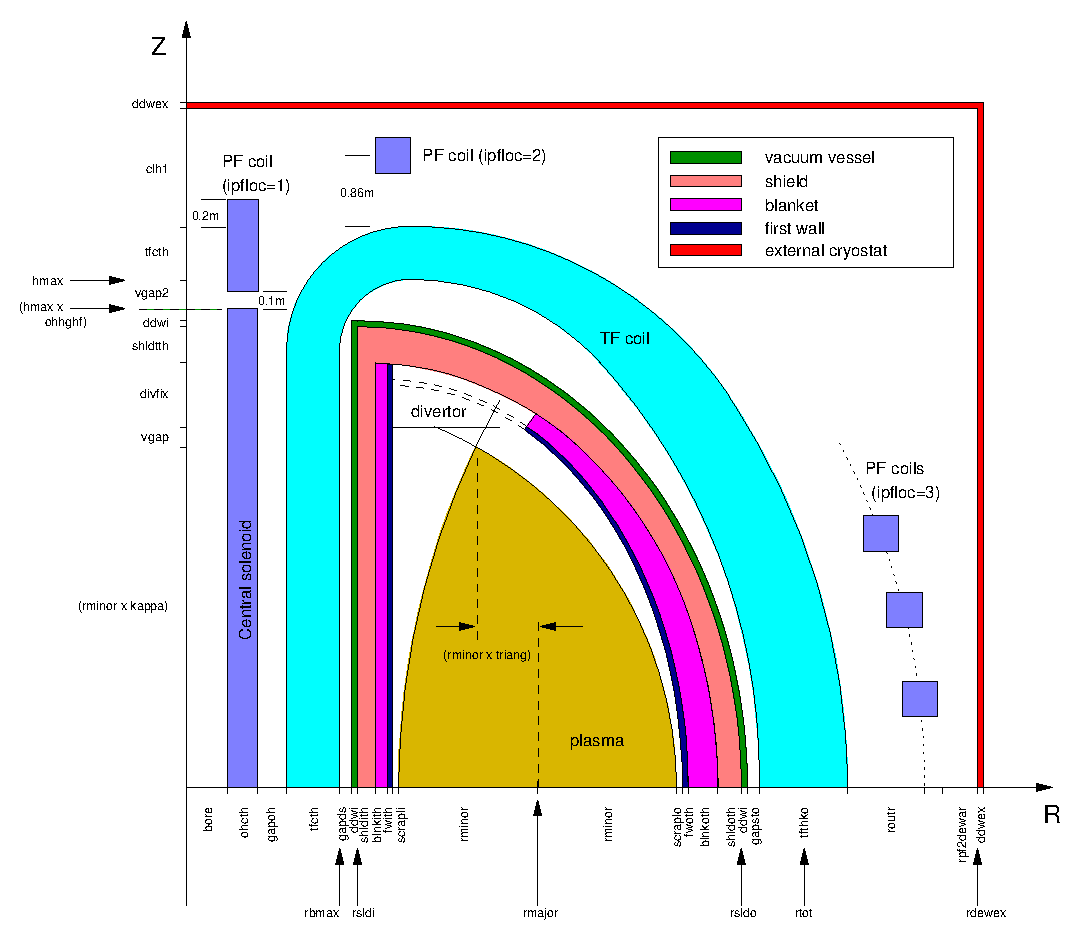
\epsfig{file=documentation/build_d.eps,width=170mm}
\caption[Machine build for D-shaped major components]
{\label{fig:build_d} \textit{Schematic diagram of the fusion
    power core of a typical tokamak power plant modelled by \process, showing
    the relative positions of the components. A double null plasma is assumed
    (\texttt{snull=0}) --- compare Figure~\ref{fig:buildsnd}, and the first
    wall, blanket, shield and vacuum vessel are D-shaped in cross-section
    (chosen by setting switch \texttt{fwbsshape=1}) --- compare
    Figure~\ref{fig:build_e}. Also shown are the code variables used to define
    the thicknesses of the components. The arrowed labels adjacent to the axes
    are the total `builds' to that point. The precise locations and sizes of
    the PF coils are calculated within the code (see
    Section~\ref{sec:pfcoils}).}  }
\end{figure}

\begin{figure}[tbph]
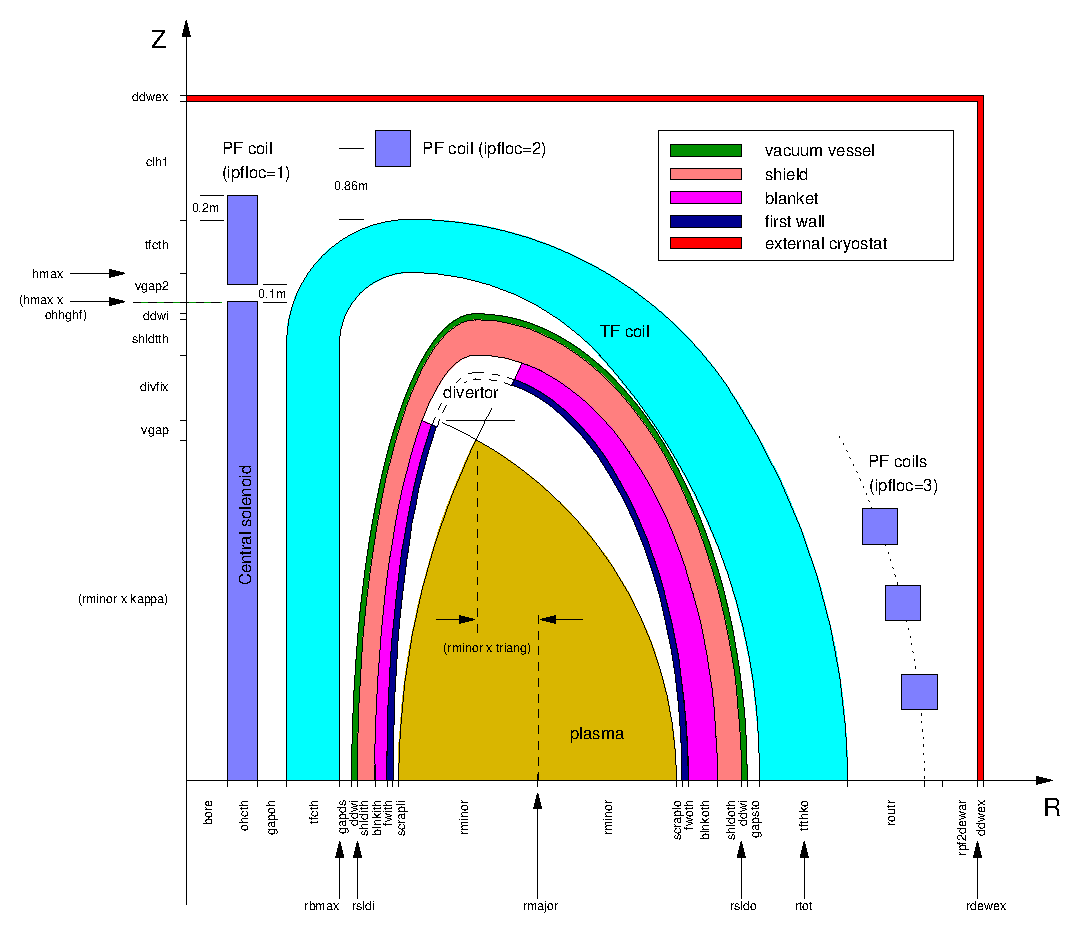
\epsfig{file=documentation/build_e.eps,width=170mm}
\caption[Machine build for elliptical-shaped major components]
{\label{fig:build_e} \textit{Schematic diagram of the fusion
    power core of a typical tokamak power plant modelled by \process. The
    first wall, blanket, shield and vacuum vessel cross-sectional shapes are
    each assumed to be defined by two ellipses (chosen by setting switch
    \texttt{fwbsshape=2}) --- compare Figure~\ref{fig:build_d}.}  }
\end{figure}

Most of the thicknesses shown in Figures~\ref{fig:build_d} and~\ref{fig:build_e}
are input parameters, so are not changed during the course of the simulation.
The rest are calculated by the code during execution. In addition, some of the
component sizes can be used as \textit{iteration variables}\/ (see
Section~\ref{sec:itvars}) to help in the optimisation process.

\begin{figure}[tbph]
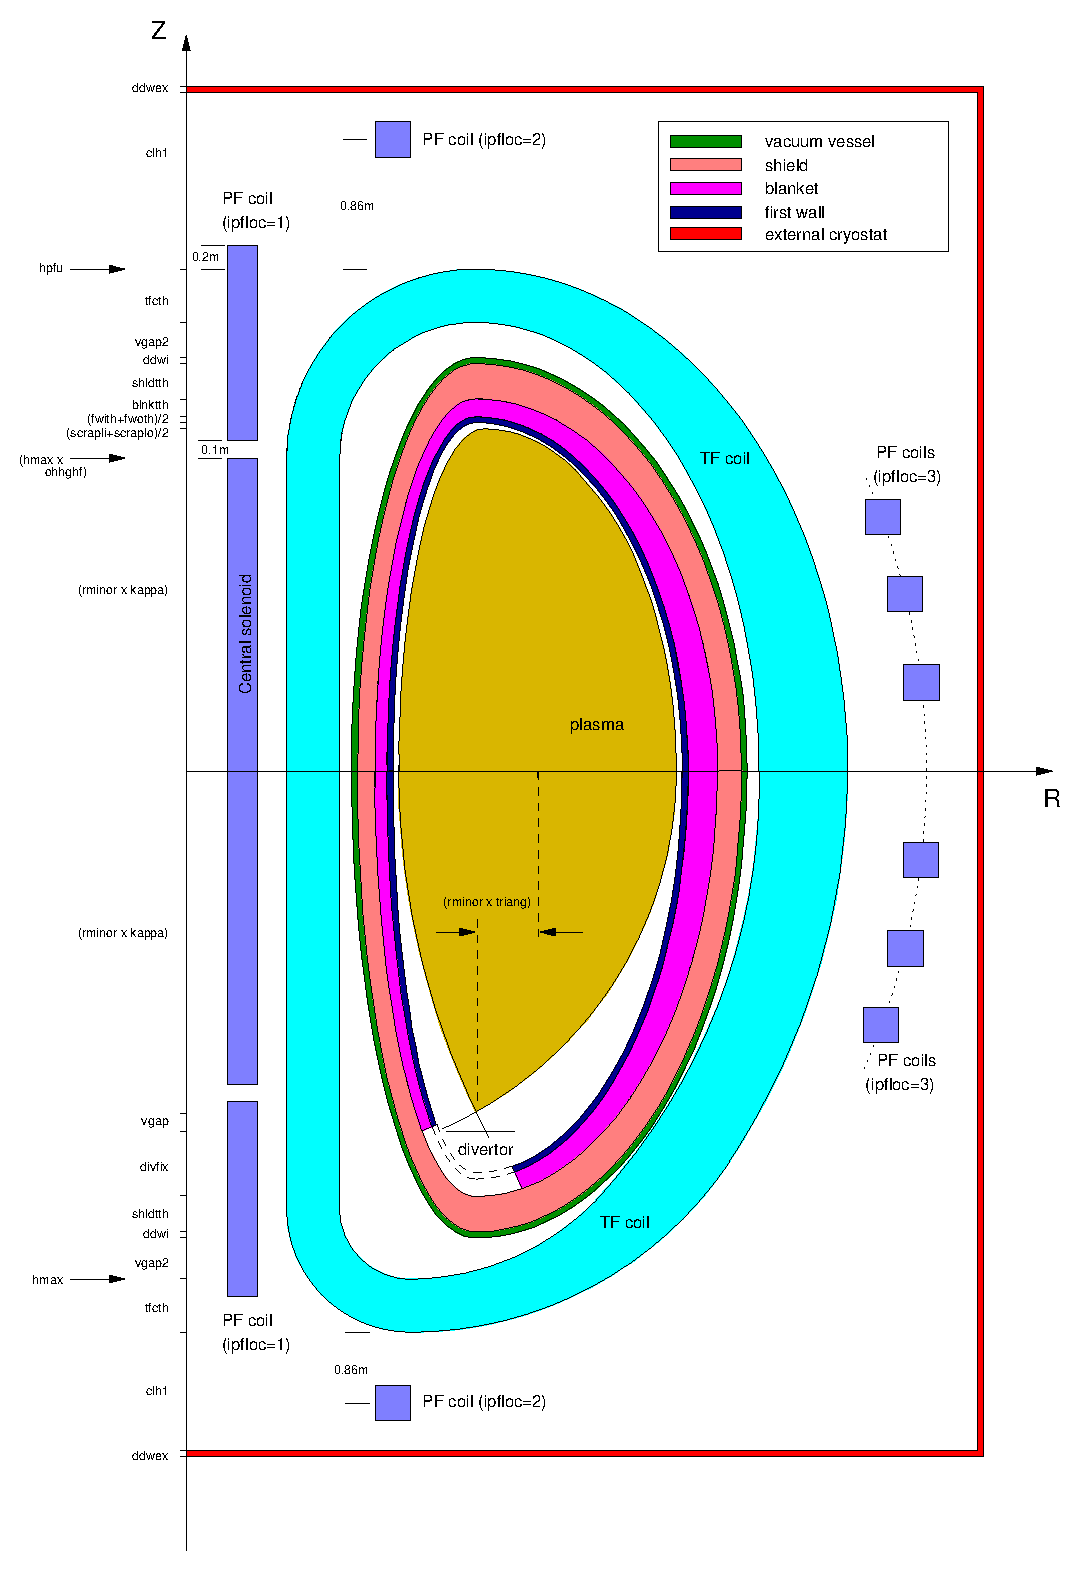
\epsfig{file=documentation/build_e_snd.eps,height=200mm}
\caption[Machine build for a single-null device]
{\label{fig:buildsnd}
  \textit{Schematic diagram of the fusion power core of a typical tokamak
    power plant modelled by \process, showing the relative positions of the
    components. A single null plasma is assumed (\texttt{snull=1}) --- compare
    Figure~\ref{fig:build_e}. The radial build is the same as for a double null
    configuration; shown along the vertical axis are the code variables used
    to define the vertical thicknesses of the components. The arrowed labels
    adjacent to the axis are the total `builds' (distance from the midplane,
    Z=0) to that point. The precise locations and sizes of the  PF coils are
    calculated within the code (see Section~\ref{sec:pfcoils}).}
}
\end{figure}

\subsection{Plasma physics models}
\label{sec:plasma_physics_models}

By default, the plasma is assumed to have an up-down asymmetric, single null
configuration (although this can be changed if desired --- see
Section~\ref{sec:divertor}). A great number of physics models are coded within
\process\ to describe the behaviour of the plasma parameters such as its
current, temperature, density, pressure, confinement etc., and also the
various limits that define the stable operating domain.

\subsubsection{Plasma geometry}
\label{sec:plasma_geometry}

The plasma (geometric) major radius $R_0$ (\texttt{rmajor}) and aspect ratio
$A$ (\texttt{aspect}) define the size of the plasma torus. The plasma minor
radius $a$ (\texttt{rminor}) is calculated from these values. The shape of the
plasma cross-section is given by its last closed flux surface (LCFS) elongation
$\kappa$ (\texttt{kappa}) and triangularity $\delta$ (\texttt{triang}), which
can be scaled automatically with the aspect ratio if required using switch
\texttt{ishape}:
\begin{itemize}

\item If \texttt{ishape = 0}, the input values for \texttt{kappa} and
  \texttt{triang} are used directly.

\item If \texttt{ishape = 1}, the following scaling is used, which is suitable
  for low aspect ratio machines ($\epsilon = 1/A$)~\cite{storac}:
\begin{eqnarray}
\kappa & = & 2.05 \, (1 + 0.44 \, \epsilon^{2.1}) \\
\delta & = & 0.53 \, (1 + 0.77 \, \epsilon^3)
\end{eqnarray}

\item If \texttt{ishape = 2}, the Zohm ITER scaling~\cite{Zohm} is used to
  calculate the elongation:
\begin{equation}
\kappa = F_{kz} \, \times \, \mathrm{minimum} \left( 2.0, \, \, 1.5 + \frac{0.5}{A-1} \right)
\end{equation}
where input variable \texttt{fkzohm} $= F_{kz}$ may be used to adjust the
scaling, while the input value of the triangularity is used unchanged.

\end{itemize}
If \texttt{ishape = 0, 1} or \texttt{2}, the values for the plasma shaping
parameters at the 95\% flux surface are calculated as
follows~\cite{DEMOPhysicsGuidelines}:
\begin{eqnarray}
\kappa_{95} & = & \kappa / 1.12 \label{eqn:k95} \\
\delta_{95} & = & \delta / 1.5 \label{eqn:d95}
\end{eqnarray}
\begin{itemize}

\item If \texttt{ishape = 3}, the Zohm ITER scaling~\cite{Zohm} is used to
  calculate the elongation (as for \texttt{ishape = 2} above), but the
  triangularity at the 95\% flux surface is input via variable
  \texttt{triang95}, and the LCFS triangularity \texttt{triang} is calculated
  from it, rather than the other way round.

\item Finally, if \texttt{ishape = 4}, the 95\% flux surface values
  \texttt{kappa95} and \texttt{triang95} are both used as inputs, and the LCFS
  values are calculated from them by inverting Equations~\ref{eqn:k95} and~\ref{eqn:d95}.

\end{itemize}

A constraint relating to the plasma's vertical stability may be turned on if
required. In principle, the inner surface of the outboard shield could be used
as the location of a conducting shell which should mitigate the vertical
displacement growth rate of plasmas with significant
elongation~\cite{Sakamoto}. The maximum distance $r_{\mbox{\scriptsize shell,
  max}}$ of this shell from the centre of the plasma may be set using input
parameter \texttt{cwrmax}, such that $r_{\mbox{\scriptsize shell, max}} = $
\texttt{cwrmax*rminor}. Constraint equation no.\ 23 should be turned on with
iteration variable no.\ 104 (\texttt{fcwr}) to enforce this. (A scaling of
\texttt{cwrmax} with elongation should be available shortly.)

The plasma surface area, cross-sectional area and volume are calculated using
formulations that approximate the LCFS as a revolution of two arcs which
intersect the plasma X-points and the plasma midplane outer and inner
radii. (This is a reasonable assumption for double-null diverted plasmas, but
will be inaccurate for single-null plasmas, \texttt{snull = 1}.) Switch
\texttt{igeom} determines whether an old method is used (\texttt{igeom = 0})
or calculations based on a more recent derivation (\texttt{igeom =
  1})~\cite{logbook14_41}.

\subsubsection{Fusion reactions}
\label{sec:fusion_reactions}

The most likely fusion reaction to be utilised in a power plant is the
deuterium-tritium reaction:
\begin{equation}
\mathrm{D + T} \Longrightarrow \mathrm{^{4}He + n + 17.6 \,MeV}
\label{eqn:d-t}
\end{equation}
20\% of the energy produced is given to the alpha particles ($^4$He), a
fraction of which remain (c.f.\ \texttt{falpha}, Section~{sec:corepower})
within the plasma and thermalise (slow down) due to collisions, thus heating
the plasma. The remaining 80\% is carried away by the neutrons, which deposit
their energy within the blanket and shield.

\process\ can also model D-$^3$He power plants, which utilise the following primary
fusion reaction:
\begin{equation}
\mathrm{D + \mbox{$^3$He}} \Longrightarrow \mathrm{^{4}He + p + 18.3 \,MeV}
\label{eqn:dhe3}
\end{equation}
The fusion reaction rate is significantly different to that for D-T fusion,
and the power flow from the plasma is modified since charged particles are
produced rather than neutrons. Because only charged particles (which remain in
the plasma) are produced by this reaction, the whole of the fusion power is
used to heat the plasma. Useful energy is extracted from the plasma since the
radiation power produced is very high, and this can be converted to
electricity in a number of ways.

Since the temperature required to ignite the D-$^3$He reaction is considerably
higher than that for D-T, it is necessary to take into account the following
D-D reactions, which have significant reaction rates at such temperatures:
\begin{eqnarray}
\mathrm{D + D} & \Longrightarrow & \mathrm{^{3}He + n + 3.27 \,MeV} \\
\mathrm{D + D} & \Longrightarrow & \mathrm{T + p + 4.03 \,MeV}
\end{eqnarray}
Also, as tritium is produced by the latter reaction, D-T fusion is also
possible. As a result, there is still a small amount of neutron power
extracted from the plasma.

Pure D-$^3$He tokamak power plants do not include blankets, because of the near
absence of neutrons leaving the plasma, and the fact that no tritium needs to
be produced for fuel.

The contributions from all four of the above fusion reactions are included in
the total fusion power production calculation. The fusion reaction rates are
calculated using the parametrizations in~\cite{BoschHale}, integrated over the
plasma profiles (correctly, with or without pedestals).

The fractional composition of the ``fuel'' ions (D, T and $^3$He) is
controlled using the three variables \texttt{fdeut}, \texttt{ftrit} and
\texttt{fhe3}, respectively:
\begin{eqnarray*}
n_{\mbox{\scriptsize fuel}} & = & n_D + n_T + n_{\mathrm{^{3}He}}  \;\;\; \mbox{particles/m$^3$} \\
n_D & = & \mathtt{fdeut} \, n_{\mbox{\scriptsize fuel}} \\
n_T & = & \mathtt{ftrit} \, n_{\mbox{\scriptsize fuel}} \\
n_{\mathrm{^{3}He}} & = & \mathtt{fhe3} \, n_{\mbox{\scriptsize fuel}}
\end{eqnarray*}
\process\ checks that \texttt{fdeut + ftrit + fhe3 = 1.0}, and stops with an
error message otherwise.

\subsubsection{Plasma profiles}

If switch \texttt{ipedestal = 0}, the plasma profiles are assumed to be
parabolic, i.e.\ they are of the form
\begin{eqnarray}
\mbox{Density : } n(\rho) & = & n_0 \left( 1 - \rho^2 \right)^{\alpha_n} \\
\mbox{Temperature : } T(\rho) & = & T_0 \left( 1 - \rho^2 \right)^{\alpha_T} \\
\mbox{Current : } J(r) & = & J_0 \left( 1 - \rho^2 \right)^{\alpha_J}
\end{eqnarray}
where $\rho = r/a$, and $a$ is the plasma minor radius. This gives
volume-averaged values $\langle n \rangle = n_0 / (1+\alpha_n)$, and
line-averaged values $\bar{n} \sim n_0 / \sqrt{(1+\alpha_n)}$, etc.  These
volume- and line-averages are used throughout the code along with the profile
indices $\alpha$, in the various physics models, many of which are fits to
theory-based or empirical scalings. Thus, the plasma model in \process\ may
be described as ``$\frac{1}{2}$-D''.  The relevant profile index variables are
\texttt{alphan}, \texttt{alphat} and \texttt{alphaj}, respectively (see
Section~\ref{sec:current_profile}).

However, by default, \texttt{ipedestal = 1} which allows the density and
temperature profiles to include a pedestal, using the forms specified
in~\cite{helios}:
\begin{equation}
\mbox{density:} \qquad n(\rho) = \left\{ 
\begin{aligned}
  &n_{ped} + (n_0 - n_{ped}) \left( 1 -
    \frac{\rho^2}{\rho_{ped,n}^2}\right)^{\alpha_n}
  &\qquad 0 \leq \rho \leq \rho_{ped,n} \\
  &n_{sep} + (n_{ped} - n_{sep})\left( \frac{1- \rho}{1-\rho_{ped,n}}\right)
  &\qquad \rho_{ped,n} < \rho \leq 1
\end{aligned}
\right.
\end{equation}

\begin{equation}
\mbox{temperature:} \qquad T(\rho) = \left\{ 
\begin{aligned}
  &T_{ped} + (T_0 - T_{ped}) \left( 1 - \frac{\rho^{\beta_T}}
    {\rho_{ped,T}^{\beta_T}}\right)^{\alpha_T} &\qquad 0 \leq \rho \leq \rho_{ped,T} \\
  &T_{sep} + (T_{ped} - T_{sep})\left( \frac{1- \rho}{1-\rho_{ped,T}}\right)
  &\qquad \rho_{ped,T} < \rho \leq 1
\end{aligned}
\right.
\end{equation}
Subscripts $0$, $ped$ and $sep$, denote values at the centre ($\rho = 0$), the
pedestal ($\rho = \rho_{ped}$) and the separatrix ($\rho=1$),
respectively. The density and temperature peaking parameters $\alpha_n$ and a
$\alpha_T$ as well as the second exponent $\beta_T$ (input parameter
\texttt{tbeta}, not to be confused with the plasma beta) in the temperature
profile can be chosen by the user, as can the pedestal heights and the values
at the separatrix (\texttt{neped, nesep} for the electron density, and
\texttt{teped, tesep} for the electron temperature; the ion equivalents are
scaled from the electron values by the ratio of the volume-averaged values).
The density at the centre is given by
\begin{eqnarray}
  \nonumber
  n_0 &= & \frac{1}{3\rho_{ped,n}^2} \left[3\langle n\rangle (1+\alpha_n)
    + n_{sep} (1+\alpha_n) (-2 + \rho_{ped,n} + \rho_{ped,n}^2) \right.\\
  && \left. - n_{ped}\left( (1 + \alpha_n)(1+ \rho_{ped,n}) + (\alpha_n -2)
    \rho_{ped,n}^2 \right) \right]
\end{eqnarray}
where $\langle n \rangle$ is the volume-averaged density. The temperature at
the centre is given by
\begin{equation}
T_0 = T_{ped} + \gamma \left[ T_{ped}\, \rho_{ped,T}^2 - \langle T \rangle +
  \frac{1}{3}(1 - \rho_{ped,T}) \left[ \, (1 + 2\rho_{ped,T}) \, T_{ped} + ( 2 +
    \rho_{ped,T}) \, T_{sep} \, \right] \right]
\end{equation}
with 
\begin{equation}
\gamma = \left\{ 
\begin{aligned}
  &\frac{ -\Gamma(1+\alpha_T+2/\beta_T)}
  {\rho_{ped,T}^2 \, \Gamma(1+\alpha_T) \, \Gamma((2+\beta_T)/\beta_T)}
  &\qquad \textnormal{for integer } \alpha_T \\
  &\frac{\Gamma(-\alpha_T)\sin(\pi\alpha)\, \Gamma(1+\alpha_T+2/\beta_T)}
  {\pi\rho_{ped,T}^2 \, \Gamma((2+\beta_T)/\beta_T)}
  &\qquad \textnormal{for non-integer } \alpha_T
\end{aligned}
\right.
\end{equation}
where $\Gamma$ is the gamma function.

Note that density and temperature can have different pedestal positions
$\rho_{ped,n}$ (\texttt{rhopedn}) and $\rho_{ped,T}$ (\texttt{rhopedt}) in
agreement with simulations.

The pedestal density can be set directly (if \texttt{iscdens=1}), or as a fraction of the Greenwald density (if \texttt{iscdens=1}).  The default fraction is 0.8~\cite{Bernert}. 

\subsubsection{Beta limits}

The plasma beta limit~\cite{IPDG,172} is given by
\begin{equation}
\langle \beta \rangle < g \, \frac{I(\mbox{MA})}{a(\mbox{m}) \, B_0(\mbox{T})}
\label{eqn:troyon}
\end{equation}
where $B_0$ is the axial vacuum toroidal field, and $\beta$ is defined with
respect to the total equilibrium $\mathbf{B}$-field~\cite{172}. The beta
coefficient $g$ is set using input parameter \texttt{dnbeta} (but see
Section~\ref{sec:current_profile}). To apply the beta limit, constraint
equation no.\ 24 should be turned on with iteration variable no.\ 36
(\texttt{fbetatry}). The limit can be applied to either the total plasma beta,
in which case switch \texttt{iculbl} should be set to 0, to only the thermal
component of the plasma beta, in which case \texttt{iculbl} should be set to
1, or to the thermal plus neutral beam components, in which case
\texttt{iculbl} should be set to 2.

\subsubsection*{Aspect ratio scaling of beta $g$ coefficient}

Switch \texttt{gtscale} determines whether the beta $g$ coefficient
\texttt{dnbeta} should scale with aspect ratio ($\mathtt{gtscale \not= 0}$),
or be fixed at the input value (\texttt{gtscale = 0}). Note that
\texttt{gtscale} is over-ridden if \texttt{iprofile = 1} (see
Section~\ref{sec:current_profile}).

\subsubsection*{Limiting $\epsilon.\beta_p$}

To apply a limit to the value of $\epsilon.\beta_p$, where $\epsilon = a/R$ is
the inverse aspect ratio, constraint equation no.\ 6 should be turned on with
iteration variable no.\ 8 (\texttt{fbeta}). The limiting value of
$\epsilon.\beta_p$ should be set using input parameter \texttt{epbetmax}.

\subsubsection{Fast alpha pressure contribution}

Switch \texttt{ifalphap} may be used to select the model used to calculate the
pressure contribution from the fast alpha particles:
\begin{eqnarray}
\frac{\beta_{\alpha}}{\beta_{th}} & = & 0.29 \, \left( \langle T_{10} \rangle -
  0.37 \right) \, \left( \frac{n_{DT}}{n_e} \right)^2
\hspace{20mm} \mbox{\texttt{ifalphap = 0}~\cite{IPDG}} \\
\frac{\beta_{\alpha}}{\beta_{th}} & = & 0.26 \, \left( \langle T_{10} \rangle -
  0.65 \right)^{0.5} \, \left( \frac{n_{DT}}{n_e} \right)^2
\hspace{16mm} \mbox{\texttt{ifalphap = 1} (default)~\cite{Ward_fastalpha2006}}
\end{eqnarray}
The latter model is a better estimate at higher temperatures.

\subsubsection{Density limits}

Several density limit models~\cite{172} are available in \process. These are
calculated in routine \texttt{CULDLM}, which is called by \texttt{PHYSICS}.
To enforce any of these limits, turn on constraint equation no.~5 with
iteration variable no.~9 (\texttt{fdene}).  In addition, switch
\texttt{idensl} must be set to the relevant value, as follows:-
\begin{description} %!%!%! find refs
\item [\texttt{idensl = 1} :] ASDEX model
\item [\texttt{idensl = 2} :] Borrass model for ITER, I
\item [\texttt{idensl = 3} :] Borrass model for ITER, II
\item [\texttt{idensl = 4} :] JET edge radiation model
\item [\texttt{idensl = 5} :] JET simplified model
\item [\texttt{idensl = 6} :] Hugill-Murakami $M.q$ model
\item [\texttt{idensl = 7} :] Greenwald model
\end{description}

\subsubsection{Impurities and radiation}
\label{sec:radiation}

The impurity radiation model in \process\/ can be chosen using the switch
\texttt{imprad\_model}, where \texttt{imprad\_model = 0} gives the original
ITER 1989 model~\cite{kovari_physics}, and \texttt{imprad\_model = 1} uses a
multi-impurity model which integrates the radiation contributions over an
arbitrary choice of density and temperature profiles~\cite{hanni_radiation}.

If \texttt{imprad\_model = 0}, the impurity species and fractions are chosen
using input parameters \texttt{impc}, \texttt{impo}, \texttt{fbfe},
\texttt{cfe0} and \texttt{zfear}; see the variable descriptor file for more
details.

If \texttt{imprad\_model = 1}, the impurity number density fractions relative
to the electron density are set using input array \texttt{fimp(1 to nimp)},
where \texttt{nimp = 14} is the number of impurity species in the radiation
model. The available impurities are as follows:
\begin{enumerate}
\item Hydrogen (fraction calculated by code)
\item Helium (fraction calculated by code)
\item Beryllium
\item Carbon
\item Nitrogen
\item Oxygen
\item Neon
\item Silicon
\item Argon
\item Iron
\item Nickel
\item Krypton
\item Xenon
\item Tungsten
\end{enumerate}
As stated above, the number density fractions for hydrogen (all isotopes) and
helium need not be set, as they are calculated by the code to ensure that
plasma quasi-neutrality is maintained, and taking into account the fuel ratios
\texttt{fdeut}, \texttt{ftrit} and \texttt{fhe3} (see
Section~\ref{sec:fusion_reactions}), and the alpha particle fraction
\texttt{ralpne} which may be input by the user.

The impurity fraction of one of the elements listed in array \texttt{fimp} may
be used as an iteration variable (although it will only have any effect if
\texttt{imprad\_model = 1}). The element to use is specified using input
parameter \texttt{impvar}, which may be set to a value between 3 and
\texttt{nimp}, and the initial estimate to use for the element's impurity
fraction must be set using iteration variable no.\ 102 (\texttt{fimpvar}).

The synchrotron radiation power~\cite{albajar, fidone} is assumed to originate
from the plasma core. The wall reflection factor \texttt{ssync} may be set by
the user.

By changing the input parameter \texttt{coreradius}, the user may set the
normalised radius defining the core region (\texttt{imprad\_model = 1}
only). Only the impurity and synchrotron radiation from the core region
affects the confinement scaling (but see the \texttt{iradloss} description in
Section~\ref{sec:iradloss}). Figure~\ref{fig:radiation} elucidates the
radiation power contributions, while Figure~\ref{fig:powerflow1} shows how the radiation power propagates through the fusion power core.

\begin{figure}[tbph]
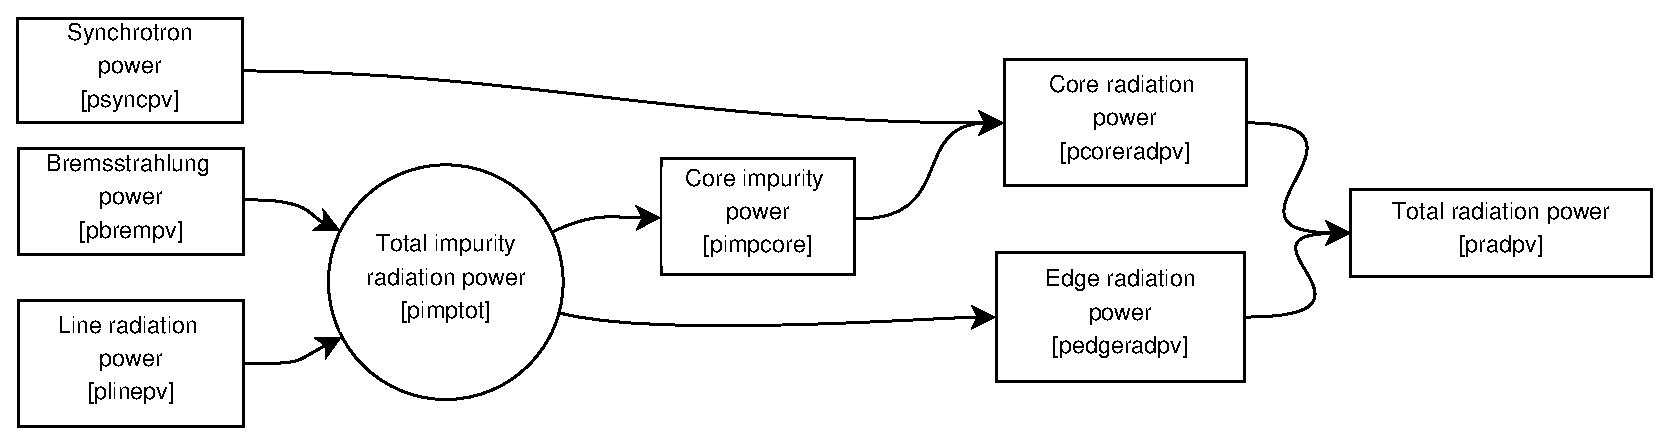
\epsfig{file=documentation/radiation.eps,width=170mm}
\caption[Radiation power contributions] {\label{fig:radiation}
  \textit{Schematic diagram of the radiation power contributions and how they
    are split between core and edge radiation, for \texttt{imprad\_model = 1}.} }
\end{figure}

Constraint equation no.~17 with iteration variable no.~28 (\texttt{fradpwr})
ensures that the calculated total radiation power does not exceed the total
power available that can be converted to radiation (i.e.\ the sum of the fusion
alpha power, other charged particle fusion power, auxiliary injected power and
the ohmic power). This constraint should always be turned on.

\subsubsection{Plasma current scaling laws}
\label{sec:current_scaling}

A number of plasma current scaling laws exploiting the inverse relationship
between plasma current and edge safety factor $q_{\psi}$~\cite{172} are
available in \process. These are calculated in routine \texttt{CULCUR}, which
is called by \texttt{PHYSICS}.  Flag \texttt{icurr} must be set to the
relevant value, as follows:-
\begin{description}
\item [\texttt{icurr = 1} :] Peng analytic fit
\item [\texttt{icurr = 2} :] Peng double null divertor scaling (ST)~\cite{storac}
\item [\texttt{icurr = 3} :] Simple ITER scaling
\item [\texttt{icurr = 4} :] Revised ITER scaling~\cite{Uckan88}
\item [\texttt{icurr = 5} :] Todd empirical scaling, I
\item [\texttt{icurr = 6} :] Todd empirical scaling, II
\item [\texttt{icurr = 7} :] Connor-Hastie model
\item [\texttt{icurr = 8} :] Sauter model, allows negative $\delta$
\end{description}

\subsubsection{Plasma current profile consistency}
\label{sec:current_profile}

Self-consistency between the plasma current profile
parameters~\cite{DEMOPhysicsGuidelines} can be enforced by setting switch
\texttt{iprofile} to 1. This ensures that the current profile peaking factor
\texttt{alphaj} is consistent with the input values for the safety factor on
axis and at the plasma edge (\texttt{q0} and \texttt{q}, respectively), the
plasma internal inductance $l_i$ is consistent with this \texttt{alphaj}, and
the beta $g$ coefficient \texttt{dnbeta} scales with $l_i$.

It is recommended that current scaling law \texttt{icurr = 4} is used if
\texttt{iprofile = 1}. Switch \texttt{gtscale} is over-ridden if
\texttt{iprofile = 1}.

\subsubsection{Confinement time scaling laws}
\label{sec:taue}

The particle transport loss power in Watts/m$^3$ from the plasma is defined as
\begin{equation}
P_{\mbox{\scriptsize loss}} = \frac{W}{\tau_E}
\label{eqn:ploss}
\end{equation}
where the plasma stored energy per unit volume $W$ is given by
\[
W = \frac{3}{2} \,n \, e \, T
\]
with particle number density $n$ in m$^{-3}$ and particle temperature $T$ in
eV. \process\ assumes that the electron and ion energy confinement times
$\tau_E$ are equal.

Many energy confinement time scaling laws are present within \process, for
tokamaks, RFPs or stellarators. These are calculated in routine
\texttt{PCOND}. The value of \texttt{isc} determines which of the scalings is
used in the plasma energy balance calculation (Section~\ref{sec:corepower}).
Table~\ref{tab:scaling_laws} summarises the available scaling laws.  The most commonly used is the so-called IPB98(y,2) scaling.

% Table summarising confinement time scaling laws in PROCESS.
\begin{table}[tbph]
\begin{center}
\footnotesize
\begin{tabular}{||c||l|l||} \hline
\texttt{isc} & scaling law & reference \\ \hline
\texttt{1}  & Neo-Alcator (ohmic) & \cite{IPDG} \\
\texttt{2}  & Mirnov (H-mode) & \cite{IPDG} \\
\texttt{3}  & Merezhkin-Muhkovatov (L-mode) & \cite{IPDG} \\
\texttt{4}  & Shimomura (H-mode) & JAERI-M 87-080 (1987) \\
\texttt{5}  & Kaye-Goldston (L-mode) & Nuclear Fusion \textbf{25} (1985) p.65 \\
\texttt{6}  & ITER 89-P (L-mode) & Nuclear Fusion \textbf{30} (1990) p.1999 \\
\texttt{7}  & ITER 89-O (L-mode) & \cite{IPDG} \\
\texttt{8}  & Rebut-Lallia (L-mode) & Plasma Physics and Controlled Nuclear Fusion
Research \\
 & &  \textbf{2} (1987) p. 187 \\
\texttt{9}  & Goldston (L-mode) & Plas.\ Phys.\ Controlled Fusion \textbf{26} (1984) p.87 \\
\texttt{10} & T10 (L-mode) & \cite{IPDG} \\
\texttt{11} & JAERI-88 (L-mode) & JAERI-M 88-068 (1988) \\
\texttt{12} & Kaye-Big Complex (L-mode) & Phys.\ Fluids B \textbf{2} (1990) p.2926 \\
\texttt{13} & ITER H90-P (H-mode) &  \\
\texttt{14} & ITER Mix (minimum of \texttt{6} and \texttt{7}) &  \\
\texttt{15} & Riedel (L-mode) &  \\
\texttt{16} & Christiansen et al. (L-mode) & JET Report JET-P (1991) 03 \\
\texttt{17} & Lackner-Gottardi (L-mode) & Nuclear Fusion \textbf{30} (1990) p.767  \\
\texttt{18} & Neo-Kaye (L-mode) & \cite{IPDG} \\
\texttt{19} & Riedel (H-mode) &  \\
\texttt{20} & ITER H90-P (amended) & Nuclear Fusion \textbf{32} (1992) p.318 \\
\texttt{21} & Large Helical Device (stellarator) & Nuclear Fusion \textbf{30} (1990)
p.11 \\
\texttt{22} & Gyro-reduced Bohm (stellarator) & Bull. Am. Phys. Society, \textbf{34}
(1989) p.1964 \\
\texttt{23} & Lackner-Gottardi (stellarator) & Nuclear Fusion \textbf{30} (1990) p.767 \\
\texttt{24} & ITER-93H (H-mode) & Plasma Physics and Controlled Nuclear Fusion Research \\
 & & (Proc. 15th Int. Conf., Seville, 1994) IAEA-CN-60/E-P-3 \\
\texttt{25} & TITAN (RFP) & TITAN RFP Fusion Reactor Study, Scoping Phase Report \\
 & & UCLA-PPG-1100, page 5--9, Jan 1987 \\
\texttt{26} & ITER H-97P ELM-free (H-mode) & J. G. Cordey et al., EPS Berchtesgaden, 1997 \\
\texttt{27} & ITER H-97P ELMy (H-mode) & J. G. Cordey et al., EPS Berchtesgaden, 1997 \\
\texttt{28} & ITER-96P (= ITER97-L) (L-mode) & Nuclear Fusion \textbf{37} (1997) p.1303 \\
\texttt{29} & Valovic modified ELMy (H-mode) &  \\
\texttt{30} & Kaye PPPL April 98 (L-mode) &  \\
\texttt{31} & ITERH-PB98P(y) (H-mode) &  \\
\texttt{32} & IPB98(y) (H-mode) & Nuclear Fusion \textbf{39} (1999) p.2175 \\
\texttt{33} & IPB98(y,1) (H-mode) & Nuclear Fusion \textbf{39} (1999) p.2175 \\
\texttt{34} & IPB98(y,2) (H-mode) & Nuclear Fusion \textbf{39} (1999) p.2175 \\
\texttt{35} & IPB98(y,3) (H-mode) & Nuclear Fusion \textbf{39} (1999) p.2175 \\
\texttt{36} & IPB98(y,4) (H-mode) & Nuclear Fusion \textbf{39} (1999) p.2175 \\
\texttt{37} & ISS95 (stellarator) & Nuclear Fusion \textbf{36} (1996) p.1063 \\
\texttt{38} & ISS04 (stellarator) & Nuclear Fusion \textbf{45} (2005) p.1684 \\
\texttt{39} & DS03 (H-mode) & Plasma Phys.\ Control.\ Fusion \textbf{50} (2008) 043001, equation 4.13 \\
\texttt{40} & Non-power law & A. Murari et al 2015 Nucl. Fusion 55 073009, \\
 & & doi:10.1088/0029-5515/55/7/073009  Table 4. \\
\texttt{41} & Petty 2008 &  C.C.~Petty 2008 Phys.\ Plasmas \textbf{15} 080501, equation 36\\
\texttt{42} & Lang 2012 & P.T.~Lang et al. 2012 IAEA conference proceeding EX/P4-01\\
\hline
\end{tabular}
\normalsize
\end{center}
\caption[List of available energy confinement scaling laws]
{\label{tab:scaling_laws}
  \textit{Summary of the energy confinement time scaling laws in \process.}
}
\end{table}

\subsubsection*{Effect of radiation on energy confinement}
\label{sec:iradloss}

Published confinement scalings are all based on low radiation pulses. A power
plant will certainly be a high radiation machine --- both in the core, due to
bremsstrahlung and synchrotron radiation, and in the edge due to impurity
seeding. The scaling data do not predict this radiation --- that needs to be
done by the radiation model. However, if the transport is very ``stiff'', as
predicted by some models, then the additional radiation causes an almost equal
drop in power transported by ions and electrons, leaving the confinement
nearly unchanged.

To allow for these uncertainties, three options are available, using the
switch \texttt{iradloss}. In each case, the particle transport loss power $P_{\mbox{\scriptsize loss}}$ (Equation~\ref{eqn:ploss}), referred to in the code as \texttt{pscaling}, is
derived directly from the energy confinement scaling law (see~\ref{sec:taue} and Figure~\ref{fig:radiation} above).

\begin{description}

\item{\texttt{iradloss = 0}:}  Total power lost is scaling power plus
  radiation:
\begin{verbatim}
pscaling + pradpv = falpha*palppv + pchargepv + pohmpv + pinjmw/vol
\end{verbatim}

\item{\texttt{iradloss = 1}:}  Total power lost is scaling power plus core
  radiation only:
\begin{verbatim}
pscaling + pcoreradpv = falpha*palppv + pchargepv + pohmpv + pinjmw/vol
\end{verbatim}

\item{\texttt{iradloss = 2}:}  Total power lost is scaling power only, with no
  additional allowance for radiation. This is not recommended for power plant
  models.
\begin{verbatim}
pscaling = falpha*palppv + pchargepv + pohmpv + pinjmw/vol
\end{verbatim}

\end{description}

\subsubsection{Plasma core power balance}
\label{sec:corepower}

Figure~\ref{fig:powerflow1} shows the flow of power as calculated by the code. (Figure~
\ref{fig:powerflow3} shows an alternative view of the power transfer outside the reactor core.)

\begin{figure}[tbph]
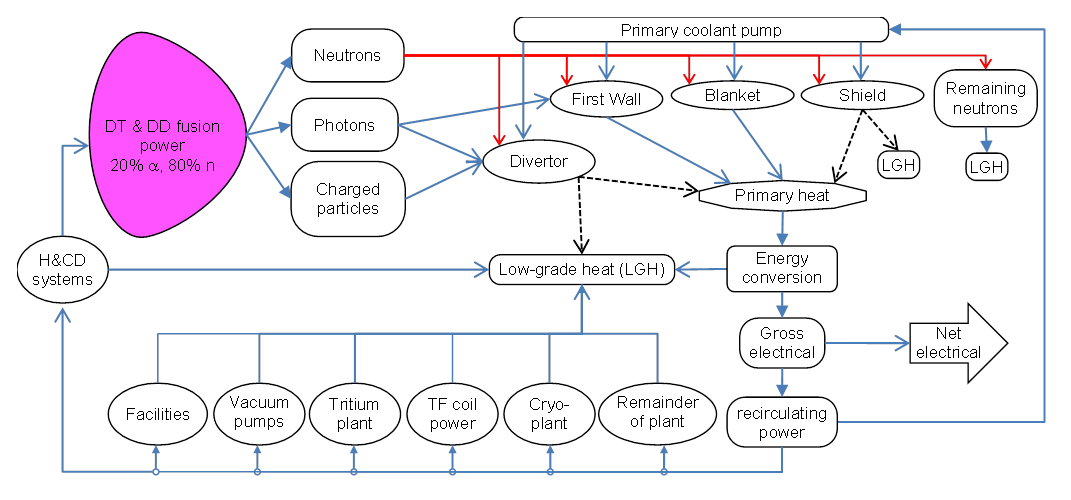
\epsfig{file=documentation/powerflow1.eps,width=170mm}
\caption[Power balance within the core plasma] {\label{fig:powerflow1}
  \textit{Power flows} }
\end{figure}

The primary sources of power are the fusion reactions themselves, ohmic power
due to resistive heating within the plasma, and any auxiliary power provided
for heating and current drive (see Section~\ref{sec:hcd}). The power carried
by the fusion-generated neutrons is lost from the plasma, but is deposited in
the surrounding material (see Section~\ref{sec:powerflow}). A fraction
\texttt{falpha} of the alpha particle power is assumed to stay within the
plasma core to contribute to the plasma power balance. The sum of this core
alpha power, any power carried by non-alpha charged particles, the ohmic power
and any injected power, is converted into charged particle transport power
($P_{\mbox{\scriptsize loss}}$ in Equation~\ref{eqn:ploss}) plus core
radiation power (see Section~\ref{sec:radiation}), as shown in
Figure~\ref{fig:powerflow1}. 

The core power balance calculation is turned on using constraint equation
no.\ 2 (which should therefore always be used).

\subsubsection{Bootstrap current scalings}
\label{sec:bootstrap}

The fraction of the plasma current provided by the so-called bootstrap effect
can be either input into the code directly, or calculated using one of four
methods, as summarised here. Note that methods \texttt{ibss = 1} to~\texttt{3}
use fits to parabolic density and temperature profiles, and do not take into
account the existence of pedestals (\texttt{ipedestal = 1}), whereas the
Sauter et al.\ scaling (\texttt{ibss = 4}) allows general profiles to be used.
\begin{itemize}

\item Direct input: To input the bootstrap current fraction directly, set
  \texttt{bscfmax} to $(-1)$ times the required value.

\item ITER scaling~\cite{IPDG}: To use the ITER scaling method for the
  bootstrap current fraction, set \texttt{ibss = 1}, and \texttt{bscfmax} to
  the maximum required bootstrap current fraction ($\leq 1$). This method is
  valid at high aspect ratio only.

\item General scaling~\cite{Nevins}: To use a more general scaling method, set
  \texttt{ibss = 2}, and \texttt{bscfmax} to the maximum required bootstrap
  current fraction ($\leq 1$).

\item Numerically fitted scaling~\cite{WilsonBS}: To use a numerically fitted
  scaling method, valid for all aspect ratios, set \texttt{ibss = 3}, and
  \texttt{bscfmax} to the maximum required bootstrap current fraction ($\leq
  1$).

\item Sauter, Angioni and Lin-Liu scaling~\cite{SauterBS, SauterBS_errata}:
  Set \texttt{ibss = 4}, and \texttt{bscfmax} to the maximum required
  bootstrap current fraction ($\leq 1$).

\end{itemize}

\subsubsection{L-H power threshold scalings}

Transitions from a standard confinement mode (L-mode) to an improved
confinement regime (H-mode), called L-H transitions, are observed in most
tokamaks. A range of scaling laws are available that provide estimates of the
auxiliary power required to initiate these transitions, via extrapolations
from present-day devices. \process\ calculates these power threshold values
for the scaling laws listed in Table~\ref{tab:power_thresholds}, in
routine~\texttt{PTHRESH}.

To enforce one of these scalings, use input parameter \texttt{ilhthresh} to
select the scaling to use, and turn on constraint equation no.\ 23 with
iteration variable no.\ 104 (\texttt{flhthresh}). By default, this will ensure
that the power reaching the divertor is at least equal to the threshold power
calculated for the chosen scaling, which is a necessary condition for
H-mode. However, for L-mode it might be appropriate to set \texttt{boundl(104)
  = 0.001, boundu(104) = 1.0}, which will ensure that the power threshold does
not exceed the calculated value, and therefore the machine cannot reach
H-mode.

% Table summarising L-H power threshold scalings

\begin{table}[tbph]
\small
\begin{center}
\begin{tabular}{||c||l||l||} \hline
 & name & reference \\ \hline
(1) & 1996 ITER scaling: nominal & ITER Physics Design Description Document, \\
(2) & 1996 ITER scaling: upper bound & D. Boucher, p.2-2 \\
(3) & 1996 ITER scaling: lower bound &  \\ \hline
(4) & 1997 ITER scaling, excluding elongation & J. A. Snipes, ITER H-mode
Threshold Database \\
(5) & 1997 ITER scaling, including elongation &  Working Group, Controlled
Fusion and Plasma \\
 & & Physics, 24th EPS Conference, Berchtesgaden, \\
 & & June 1997, vol.21A, part III, p.961 \\ \hline
(6) & 2008 Martin scaling: nominal & Martin et al, 11th IAEA Tech. Meeting on
H-mode \\
(7) & 2008 Martin scaling: 95\% upper bound &  Physics and Transport Barriers,
Journal of Physics: \\
(8) & 2008 Martin scaling: 95\% lower bound & Conference Series \textbf{123}
(2008) 012033 \\
\hline
\end{tabular}
\end{center}
\normalsize
\caption[List of available L-H power threshold scalings]
{\label{tab:power_thresholds}
  \textit{Summary of the L-H power threshold scalings implemented in \process.}
}
\end{table}

\subsubsection{Other plasma physics options}

\subsubsection*{Neo-classical correction effects}

Switch \texttt{ires} controls whether neo-classical (trapped particle) 
effects~\cite{Uckan} are included in the calculation of the plasma resistance
and ohmic heating power in routine \texttt{POHM}, which is called by routine
\texttt{PHYSICS}. If \texttt{ires = 1}, these effects are included. Note that
the scaling used is only valid for aspect ratios between 2.5 and 4, and it is
possible for the plasma resistance to be wrongly calculated as negative if
\texttt{ires = 1} and the aspect ratio is too high.

\subsubsection*{Inverse quadrature in $\tau_E$ scaling laws}

Switch \texttt{iinvqd} determines whether the energy confinement time scaling
laws (see Section~\ref{sec:taue}) due to Kaye-Goldston (\texttt{isc = 5}) and
Goldston (\texttt{isc = 9}) should include an inverse quadrature scaling with
the Neo-Alcator result (\texttt{isc = 1}). A value \texttt{iinvqd = 1}
includes this scaling.

\subsubsection*{Plasma / first wall gap}

The region directly outside the last closed flux surface of the core plasma is
known as the scrape-off layer, and contains no structural material.  Plasma
entering this region is not confined and is removed by the divertor. \process\
treats the scrape-off layer merely as a gap. Switch \texttt{iscrp} determines
whether the inboard and outboard gaps should be calculated as 10\% of the
plasma minor radius (\texttt{iscrp = 0}), or set equal to the input values
\texttt{scrapli} and \texttt{scraplo} (\texttt{iscrp = 1}).

\subsection{PLASMOD - 1D transport model}
\label{sec:plasmod}

The PLASMOD~\cite{PLASMOD} code is a one-dimensional, time-independent particle and energy transport model, which has some basis in the ASTRA~\cite{ASTRA} simulator. Even this simplified transport code leads to potentially much more accurate modelling of the fusion power generated when compared to the 0D approximations found elsewhere in \process. PLASMOD solves for a user-defined number of discrete points in the radial direction between the core of the plasma and the pedestal in order to create profiles which are not based on simple parameterizations.

Switch \texttt{ipedestal = 2} requests that PLASMOD be run \textit{only after} \process\ has found a feasible solution, whereas if \texttt{ipedestal = 3} then PLASMOD is called during every \process\ iteration. It is recommended that \texttt{ipedestal = 3} be used, other than for testing purposes.

PLASMOD is run in conjunction with many \process\ physics models, although certain constraints and iteration variables are not applicable when \texttt{ipedestal = 3}, as detailed in this section. Engineering models are unaffected, although naturally, results in all model-types are liable to change.

\subsubsection*{PLASMOD inputs}
User-defined inputs specific to PLASMOD have the prefix 'plasmod\_' and should be added to the \indat. These control various aspects of the transport simulation, from maximum number of iterations to be attempted to the current drive efficiency. For a complete list refer to the vardes.html file.

\subsubsection*{PLASMOD switches}
Here is a summary of sub-models which may be accessed by the user:

\begin{itemize}
\item \texttt{plasmod\_i\_equiltype} Equilibrium model: 1 - EMEQ, solve with sawteeth and inputted q95. 2 - EMEQ, solve with sawteeth and inputted Ip (not recommended).
\item \texttt{plasmod\_i\_modeltype} Transport model: 1 - Simple gyrobohm scaling with imposed H factor $>$ 1. Other values give H factor as output. 111 - roughly calibrated to give H=1 for DEMO, but not fixed H.
\item \texttt{plasmod\_iprocess} Sub-functions: 0 - use PLASMOD functions, 1 - use PROCESS functions.
\item \texttt{plasmod\_i\_impmodel} Impurity model: 0 - fixed concentration, 1 - fixed concentration at pedestal top, then fixed density. 
\item \texttt{plasmod\_isawt} Sawtooth modelling: 0 - none, 1 - solve with sawteeth.  
\end{itemize}

For more details refer to the vardes.html file.

\subsubsection*{PROCESS physics models substituted by PLASMOD}
With reference to the sections found in~\ref{sec:plasma_physics_models} this is a summary of key outputs from PLASMOD:

\begin{itemize}
\item Plasma geometry - $\kappa$ and $\delta$
\item Fusion reactions - power from D + T, D + D, ???...interactions are calculated by PLASMOD
\item Plasma profiles - all radial profiles are created by PLASMOD, including many not availabe in \process\ 0D: electron density, electron temperature, ion density, ion temperature, current density, bootstrap current, current from current drive, poloidal current, poloidal fluix, safety factor, plasma conductivity, alpha pressure...
\end{itemize}

\subsubsection*{PROCESS physics models used by PLASMOD}

\begin{itemize}
\item Pedestal pressure scaling (subroutine \texttt{p\_eped\_scaling})
\item Radiation model for Bremsstrahlung (subroutine \texttt{impradprofile})
\item L-mode to H-mode power threshold calculation (subroutine \texttt{pthresh})
\item Fusion reaction rate calculation (function \texttt{bosch\_hale})
\end{itemize}

\subsubsection*{PROCESS physics models constrained when using PLASMOD}

\begin{itemize}

\item The following iteration variables may not be used, as they are outputs of PLASMOD:
  \subitem 4    \texttt{te}
  \subitem 5    \texttt{beta}
  \subitem 6    \texttt{dene}
  \subitem 9    \texttt{fdene}
  \subitem 44   \texttt{fvsbrnni}
  \subitem 102  \texttt{fimpvar}
  \subitem 103  \texttt{flhthresh}
  \subitem 109  \texttt{ralpne}
  \subitem 110  \texttt{ftaulimit}

\item The following constraint equations may not be used, as they are constrained within PLASMOD:
  \subitem 1    Beta
  \subitem 2    Global power balance
  \subitem 5    Density upper limit
  \subitem 15   LH power threshold limit
  \subitem 24   Beta upper limit
  \subitem 30   Injection power upper limit ???
  \subitem 62   Ratio of particle to energy confinement time
  \subitem 68   Pseparatrix * Bt / q*A*R
  

\item If \texttt{plasmod\_i\_modeltype} $>$1 no constraint equations relating to beta may be applied.
  
\item Only \texttt{ishape = 4} may be used.

\item NBI heating must be applied with the flag \texttt{iefrf} set to model 5 (ITER neutral beam model) or model 8 (Culham neutral beam model); Electron/Ion Cyclotron heating is not currently available in PLASMOD.

\item Switch \texttt{iradloss} must be set to 0.

\item L-H mode power threshold scaling mode must be 2008 Martin scaling: nominal (\texttt{ilhthresh} = 6).

\item Both \texttt{fgwsep} and \texttt{fgwped} must be given a value greater than 0, and \texttt{fgwped} must have the larger value.

\item Control power may be defined by the user by setting either \texttt{contrpovs} or \texttt{contrpovr} (per unit area or unit distance respectively) to be non-zero, but not both.
  

\end{itemize}

\subsection{Armour, first wall and breeding blanket}
The surface facing the plasma is a thin layer of a material highly resistant to melting and erosion, such as tungsten, referred to "armour".  It is cooled by conduction to the first wall underneath.

The first wall sits behind the armour, and is dedicated to removing the heat landing on the armour.  It does not breed tritium.  Due to the hostile environment the first wall and armour have only a short lifetime and therefore need to be replaced regularly. It is cooled either by gaseous helium or by pressurised liquid water, depending on the selection of blanket type using the switch \texttt{blkttype}  -- see Section~\ref{sec:blanket_switches}.

\subsubsection*{Wall load calculation}

Switch \texttt{iwalld} determines whether the neutron wall load (power per
unit area) should be calculated using the plasma surface area (\texttt{iwalld
  = 1}) or the first wall area (\texttt{iwalld = 2}) as the denominator. In
the former case, input parameter \texttt{ffwal} (default value 0.92)
can be used to scale the neutron power reaching the first wall.

The breeding blanket performs a number of tasks. An incoming neutron from a
deuterium-tritium (D-T) fusion reaction in the plasma loses energy in the
blanket. This energy is removed by the blanket coolant and used to produce
electricity. The neutron may also react with a lithium nucleus present in the
blanket to produce (``breed'') a tritium nucleus which can be re-used as
fuel. The competing requirements of heating and tritium synthesis mean that a
neutron multiplier must be present, to ensure balance between tritium
destruction and creation. The blanket therefore contains beryllium to fulfil
this purpose. As with the first wall, the blanket has a relatively short
lifetime because of the high neutron fluence.

\subsubsection{Blanket model options}
\label{sec:blanket_switches}

The models used for the thermoydraulics of the first wall, the profile of deposition of the neutron energy, tritium breeding, and conversion of heat to electricity have been revised extensively.
\begin{description}

\item{\texttt{iblanket}:} This switch selects between different types of blanket.

In the CCFE HCPB (helium-cooled pebble bed) model (\texttt{iblanket = 1}), the energy deposition in the armour and first wall, blanket and shield are calculated using parametric fits to an MCNP neutron and photon transport model of a sector of a tokamak.  The blanket contains lithium orthosilicate Li$_4$SiO$_4$, titanium beryllide TiBe$_{12}$, helium and Eurofer steel. 

The KIT HCPB model (\texttt{iblanket = 2}) allows the energy multiplication factor \texttt{emult}, the shielding requirements and tritium breeding ratio to be calculated self-consistently with the blanket and shielding materials and sub-assembly thicknesses, and for constraints to be applied to satisfy the engineering requirements. For further details of this model, see Section~\ref{sec:blanket_neutronics}.

The CCFE HCPB model with tritium breeding ratio (\texttt{iblanket = 3}) has the features of the CCFE HCPB model above, with a set of fitting functions for calculating tritium breeding ratio (TBR).  It requires a choice of \texttt{iblanket\_thickness}, specifiying a THIN, MEDIUM or THICK blanket.  This fixes the values of inboard and outboard blanket thickness, and the initial values of first wall thickness (3 cm) and first wall armour (3 mm).  Note that these last two can be modified by the first wall thermohydraulic module, in which case the output will not be fully self-consistent.  The lithium-6 enrichment and the breeder fraction (Li4SiO4/(Be12Ti+Li4SiO4) by volume) are available as iteration variables, and the minimum TBR can be set as a constraint.  The maximum values of TBR achievable are as follows:\\
Thin: 1.247, Medium: 1.261, Thick: 1.264.

\item{\texttt{secondary\_cycle }:} This switch controls how the coolant pumping power in the first wall and blanket is determined, and also how the calculation of the plant's thermal to electric conversion efficiency (the secondary cycle thermal efficiency) proceeds. See Section~\ref{sec:powerflow}.
 
\end{description}

\subsubsection{KIT Blanket neutronics model}
\label{sec:blanket_neutronics}

The model used if \texttt{blktmodel = 1} is based on the Helium-Cooled Pebble
Bed (HCPB) blanket concept developed by KIT (a second advanced model ---
Helium-Cooled Lithium Lead, HCLL --- will be implemented in due course). The
blanket, shield and vacuum vessel are segmented radially into a number of
sub-assemblies. Moving in the direction away from the plasma/first wall, these
are:
\begin{itemize}

\item Breeding Zone (BZ) (which includes the first wall), with radial
  thicknesses (inboard and outboard, respectively) \texttt{fwith+blbuith},
  \texttt{fwoth+blbuoth}. This consists of beryllium (with fraction by volume
  \texttt{fblbe}), breeder material (\texttt{fblbreed}), steel
  (\texttt{fblss}) and helium coolant. Three forms of breeder material are
  available: lithium orthosilicate (Li$_4$SiO$_4$) (chosen by setting
  \texttt{breedmat = 1}), lithium metatitanate (Li$_2$TiO$_3$)
  (\texttt{breedmat = 2}) or lithium zirconate (Li$_2$ZrO$_3$)
  (\texttt{breedmat = 3}). The $^6$Li enrichment percentage may be modified
  from the default 30\% using input parameter \texttt{li6enrich}.

\item Box Manifold (BM), with radial thicknesses (inboard and outboard,
  respectively) \texttt{blbmith}, \texttt{blbmoth} and helium fractions
  \texttt{fblhebmi}, \texttt{fblhebmo} (the rest being steel).

\item Back Plate (BP), with radial thicknesses (inboard and outboard,
  respectively) \texttt{blbpith}, \texttt{blbpoth} and helium fractions
  \texttt{fblhebpi}, \texttt{fblhebpo} (the rest being steel).

Together, the BZ, BM and BP make up the `blanket', with total radial
thicknesses \texttt{blnkith} (inboard) and \texttt{blnkoth} (outboard), and
void (coolant) fraction \texttt{vfblkt}; Note that these
quantities are \textit{calculated}\ from the sub-assembly values if
\texttt{blktmodel > 0}, rather than being input parameters.

\item Low Temperature Shield and Vacuum Vessel (lumped together for these
  calculations), with radial thicknesses (inboard and outboard, respectively)
  \texttt{shldith+ddwi}, \texttt{shldoth+ddwi} and \textbf{water} coolant
  fraction \texttt{vfshld} (the rest being assumed to be steel for its mass
  calculation; the neutronics model assumes that the shield contains 2\% boron
  as a neutron absorber, but this material is not explicitly mentioned
  elsewhere in the code --- so its cost is not calculated, for example).

  \textit{N.B.\ The fact that water is assumed to be the coolant in the
    shield, whereas helium is the coolant in the blanket, leads to an
    inconsistency when specifying the coolant type via switch \texttt{coolwh}
    (see Section~\ref{sec:blanket_switches}). At present we mitigate this by
    forcing \texttt{coolwh=2} (making water the coolant), as in this case the
    coolant mass and pumping costs are higher, giving the more pessimistic
    solution with regards to costs.}

\end{itemize}

A few other input parameters are useful for tuning purposes, as follows:
\begin{itemize}

\item \texttt{fvolsi} and \texttt{fvolso} are the area (and volume) coverage
  factors for the inboard and outboard shields, respectively.

\item \texttt{fvoldw} is a multiplier for the volume of the vacuum vessel,
  used in the item's mass calculation to account for ports, etc.

\item \texttt{npdiv} is the number of divertor ports, used in the calculation
  of the tritium breeding ratio.

\item \texttt{nphcdin} and \texttt{nphcdout} are the number of heating/current
  drive ports on the inboard and outboard sides, respectively, used in the
  calculation of the tritium breeding ratio. These may be either `small'
  (\texttt{hcdportsize = 1}) or `large' (\texttt{hcdportsize = 2}).

\item \texttt{wallpf} is the neutron wall load peaking factor (maximum/mean),
  used in the calculation of the blanket lifetime.

\item \texttt{ucblbreed} is the unit cost (\$/kg) of the breeder material.

\end{itemize}

\subsubsection*{KIT model outputs and available constraints}

The KIT blanket neutronics model provides the following outputs:
\begin{itemize}

\item The total nuclear power deposited in the blanket and shield,
  \texttt{pnucblkt} and \texttt{pnucshld}, respectively, and the energy
  multiplication factor in the blanket, \texttt{emult} aref calculated.

\item The tritium breeding ratio, \texttt{tbr}. This can be constrained to be
  no less than a certain value \texttt{tbrmin} for tritium self-sufficiency by
  turning on constraint equation no.\ 52 with iteration variable no.\ 89
  (\texttt{ftbr}). The inboard and outboard blanket BZ thicknesses,
  \texttt{blbuith} and \texttt{blbuoth} can also be used as iteration
  variables (90 and 91, respectively) to help the constraint to be met.

\item The tritium production rate in grammes/day is calculated.

\item The fast neutron fluence (neutrons/m$^2$) on the TF coils is
  calculated. The peak value of this quantity may be constrained to be no more
  than a maximum value \texttt{nflutfmax} by turning on constraint equation
  no.\ 53 with iteration variable no.\ 92 (\texttt{fflutf}). The inboard and
  outboard shield thicknesses, \texttt{shldith} and \texttt{shldoth} can also
  be used as iteration variables (93 and 94, respectively) to help the
  constraint to be met. (Note that in this calculation the TF coil case
  surrounding the superconductor winding pack is ignored.)

\item The nuclear heating power (MW/m$^3$) on the inboard and outboard TF
  coils is calculated. Again, this can be limited to be no more than a maximum
  value \texttt{ptfnucmax} by turning on constraint equation no.\ 54 with
  iteration variable no.\ 95 (\texttt{fptfnuc}). The inboard and outboard
  shield thicknesses also help this constraint to be met.  (Note that in this
  calculation the TF coil case surrounding the superconductor winding pack is
  ignored.) This constraint equation may also be used with \texttt{blktmodel =
    0}.

\item The helium concentration in the vacuum vessel at the end of the plant
  lifetime is calculated. This needs to be constrained for re-weldability
  purposes, and can be kept below a maximum value \texttt{vvhealw} by turning
  on constraint equation no.\ 55 with iteration variable no.\ 96
  (\texttt{fvvhe}).

\item The blanket lifetime is calculated, assuming a maximum allowable level
  of neutron damage to its steel of 60~dpa (currently not adjustable). (For
  the \texttt{blktmodel = 0} model, the allowable blanket fluence
  \texttt{abktflnc} in MW-years/m$^2$ may be input.)

\end{itemize}

\subsection{Shield}

The shield reduces the neutron flux reaching the vacuum vessel, TF coils and beyond. This minimises the radiological impact of the neutrons, and their heating of the TF coils which, if superconducting, need to remain at liquid helium temperatures. As with the blanket the energy deposited in the coolant may or may not be used to produce electricity, depending on the value of the switch \texttt{iprimshld} . The shield coolant fraction by volume is set via the input parameter \texttt{vfshld}.

The inboard and outboard shield thicknesses (\texttt{shldith} and
\texttt{shldoth}, respectively) may be used as iteration variables.

\subsection{Divertor}
\label{sec:divertor}

The divertor provides a means of removing plasma reaching the scrape-off layer. The principal outputs from the code are the divertor heat load, used to determine its lifetime, and its peak temperature. The divertor is cooled either by gaseous helium or by pressurised water.

Switch \texttt{snull} controls the overall plasma configuration. Setting
\texttt{snull = 0} corresponds to an up-down symmetric, double null
configuration, while \texttt{snull = 1} (the default) assumes a single null
plasma with the divertor at the bottom of the machine. The vertical build (see
Figure~\ref{fig:buildsnd}) and PF coil current scaling algorithms take the
value of this switch into account, although not the plasma geometry at
present.

The Harrison-Kukushkin-Hotston divertor model~\cite{IPDG} developed for ITER is available, but is unlikely to be relevant for a reactor.

\subsection{Toroidal field coils}
\label{sec:tfcoil}

The toroidal field (TF) coils can be either resistive or
superconducting. Switch \texttt{itfsup} should be set to \texttt{1} for
superconducting coils, or \texttt{0} for purely copper coils. In the
superconductor model, the \textit{CICC}\/ (Conductor In Cable Conduit)
structure shown in Figure~\ref{fig:CICC} is assumed, and the coils are cooled
using a liquid helium cryogenic system.

The steel radial plates shown in the figure help in the winding process and
also provide extra support against tangential stresses. Iteration
variable no.\ 101 (\texttt{prp}) is the ratio of the total radial plate plus
steel cap cross-sectional area within the winding pack to the total winding
pack cross-sectional area; from this, the half-thickness \texttt{trp} is
calculated.

The outboard leg of the TF coil is assumed to be the same width in the
toroidal direction as the outside edge of the inboard leg. In the radial
direction, for resistive TF coils the input parameter \texttt{tfootfi} gives
the ratio of the outboard leg thickness to the inboard leg thickness
\texttt{tfcth}; for superconducting coils the outboard thickness is set equal
to the inboard thickness.

\begin{figure}[tbph]
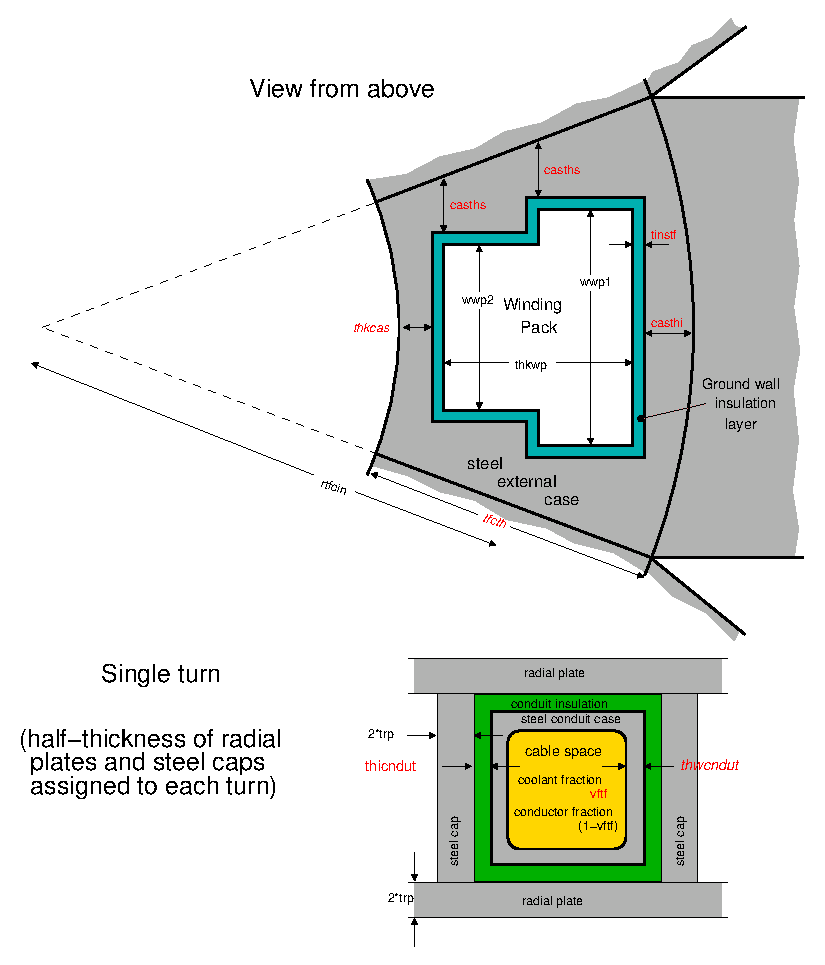
\epsfig{file=documentation/tokamak_tfcoil.eps,width=160mm}
\caption[Schematic diagram of the cross-section of a superconducting TF coil
inner leg]
{\label{fig:CICC}
  \textit{Schematic diagram of the cross-section of the inboard leg of a
    superconducting TF coil, showing the CICC (Conductor In Cable Conduit)
    construction. The winding pack contains many turns of cable conduit. The
    cable space contains the superconducting filaments, and circulating liquid
    helium coolant. The variables shown in \Red{red} may be changed by the
    user, and those in italics may be chosen as iteration variables.}
}
\end{figure}

Each TF coil is defined in the $(R,Z)$ plane by a straight section and four elliptical arcs. Because of the finite
number of TF coils used in a tokamak (18 for ITER), the toroidal field
has a ripple introduced into it, the amplitude of which can be limited to a
few percent (given by input parameter \texttt{ripmax}, default value 1\%) by
the code by adjusting the outboard gap thickness (labelled \texttt{gapsto} in
Figures~\ref{fig:build_d} and~\ref{fig:build_e}).

Among the TF coil parameters calculated by the code are the maximum allowable
current density, the stresses on the structure, the energy stored and the
magnetic field produced by the coils.

The following options are available within the superconducting TF coil model
(\texttt{itfsup = 1}).

\subsubsection{Superconducting materials}
\label{sec:superconductors}

Switch \texttt{isumattf} specifies which superconducting material is to be
used:
\begin{description}
\item [\texttt{isumattf = 1} :] Nb$_3$Sn superconductor, ITER critical surface
  parameterization~\cite{iter_nb3sn}, standard critical values
\item [\texttt{isumattf = 2} :] Bi-2212 high temperature superconductor %!%!%! ref
\item [\texttt{isumattf = 3} :] NbTi superconductor
\item [\texttt{isumattf = 4} :] Nb$_3$Sn superconductor, ITER critical surface
  parameterization~\cite{iter_nb3sn}, user-defined critical parameters
\end{description}
The fraction of copper present in the superconducting filaments is given by
the value of variable \texttt{fcutfsu} (iteration variable no.\ 59).

For \texttt{isumattf = 2}, a technology adjustment factor \texttt{fhts} may be
used to modify the critical current density fit for the Bi-2212
superconductor, to describe the level of technology assumed (i.e.\ to account
for stress, fatigue, radiation, AC losses, joints or manufacturing variations).
The default value for \texttt{fhts} is 0.5 (a value of 1.0 would be very
optimistic).

For \texttt{isumattf = 4}, important superconductor properties may be input by
the user as follows: the upper critical field at zero temperature and strain
is set using input parameter \texttt{bcritsc}, and the critical temperature at
zero field and strain is set using input parameter \texttt{tcritsc}.

\subsubsection{Current density limits}

The current in the TF coils must be sufficient to produce the required
toroidal field at the centre of the plasma. In tokamaks, the field falls off
at a rate $1/R$, with the peak value occurring at the outer edge of the
inboard portion of the TF coil winding pack ($R_{\mbox{\scriptsize max TF}} =
\mathtt{rbmax}$). The maximum TF coil current depends on the field it produces
and the allowable current density.

\newcommand{\jop}{$J_{\mbox{\scriptsize op}}$ }
\newcommand{\jcrit}{$J_{\mbox{\scriptsize crit}}$}

Three constraints are relevant to the operating current density \jop\ in the
(superconducting) TF coils.
\begin{itemize}

\item To ensure that \jop\ does not exceed the critical value \jcrit, constraint
  equation no.\ 33 should be turned on with iteration variable no.\ 50
  (\texttt{fiooic}).

\item To ensure that \jop\ does not exceed the current density protection limit,
  constraint equation no.\ 35 should be turned on with iteration variable no.\
  53 (\texttt{fjprot}).

\item The critical current density \jcrit\ falls with the temperature of the
  superconductor. The temperature margin $\Delta T$ is the difference between the
  temperature at which \jcrit would be equal to \jop\ and the operating
  temperature. The minimum allowed $\Delta T$ can be set using input parameter
  \texttt{tmargmin} together with constraint equation no.\ 36 and iteration
  variable no.\ 54 (\texttt{ftmargtf}).

  Note that if the temperature margin is positive, \jop\ is guaranteed to be
  lower than \jcrit, and so constraints~33 and~36 need not both be turned on
  (in fact, it is recommended that only one of these two constraints is
  activated in any given run).

\end{itemize}

\subsubsection{Stress model}

Switch \texttt{tfc\_model} controls whether a simple stress model
(\texttt{tfc\_model = 0}, suitable for solid copper TF coils) or a more
complex stress model (\texttt{tfc\_model = 1}) should be used. If
\texttt{tfc\_model = 1}, a two-layer stress model~\cite{Morris_tfc} developed
by CCFE is used.

To enforce the stress limits calculated using either of these models,
constraint equation no.\ 31 (case stress) and/or constraint equation no.\ 32
(conduit stress) should be turned on with iteration variables no.\ 48
(\texttt{fstrcase}) and/or no.\ 49 (\texttt{fstrcond}), respectively. The
stress limit is set using input parameter \texttt{alstrtf}.

\subsection{Poloidal field coils}
\label{sec:pfcoils}

The poloidal field (PF) coils are used initially to cancel the vertical field
produced at the centre of the plasma by the central solenoid (Section~\ref{sec:ohcoil})
during start-up, and then to maintain the plasma position and shape during the
flat-top period.

\subsubsection{PF coil positions}

The positions and sizes of the PF coils are partly input, and partly
calculated after consideration of the required currents and allowable current
density.

The PF coil locations are controlled using a set of switches stored in array
\texttt{ipfloc} (see Figure~\ref{fig:build_d}), and are calculated in routine
\texttt{PFCOIL}. The coils are (usually) organised into groups containing two
PF coils placed symmetrically above and below the midplane, and each group
\texttt{j} has an element \texttt{ipfloc(j)} assigned to it. Input parameter
\texttt{ngrp} should be set to the number of groups, and \texttt{ncls(j)}
should be assigned the number of coils in each group --- which should be
\texttt{2} in each case.

In the following, all variables are defined in the variable descriptor file
\texttt{vardes.html}. The values for \texttt{rpf1}, \texttt{rpf2},
\texttt{zref(j)} and \texttt{routr} should be adjusted by the user to locate
the PF coils accurately.

The three possible values of \texttt{ipfloc(j)} correspond to the following PF
coil positions: (\Red{Redo taking into account snull and other recent changes
  e.g. rclsnorm})
\begin{description} %!%!%! check this

\item [\texttt{ipfloc(j) = 1} :]  PF coils are placed above the central solenoid (one
group only);
\begin{eqnarray*}
R & = & \mathtt{rohc + rpf1} \\
Z & = & \pm
\mathtt{( hmax*ohhghf + 0.1 + 0.5*( hmax*(1-ohhghf)+tfcth+0.1) )}
\end{eqnarray*}

\item [\texttt{ipfloc(j) = 2} :]  PF coils are placed above the TF coils (one
group only);
\begin{eqnarray*}
R & = & \mathtt{rmajor + rpf2*triang*rminor} \hspace{62mm} \\
Z & = & \pm (\mathtt{hmax + tfcth + 0.86})
\end{eqnarray*}

\item [\texttt{ipfloc(j) = 3} :]  PF coils are placed radially outside the TF
coils (any number of groups \Red{(?)});
\begin{eqnarray*}
R & = & \mathtt{rtot + tfthko/2 + routr} \hspace{63mm}\\
Z & = & \pm(\mathtt{rminor*zref(j)})
\end{eqnarray*}

\end{description}

The void fraction (for coolant) in each coil \texttt{i}'s winding pack is
given by \texttt{vf(i)}.

\subsubsection{PF coil currents}

The peak current per turn, \texttt{cptdin(i)}, and the winding pack peak
current density \texttt{rjconpf(i)} in each PF coil \texttt{i} are inputs. The
PF coil currents vary as a function of time during the tokamak operation as
indicated in Figure~\ref{fig:current_vs_time}. They contribute part of the
flux swing necessary to maintain the plasma current (see
Section~\ref{sec:ohcoil}).

\begin{figure}[tbph]
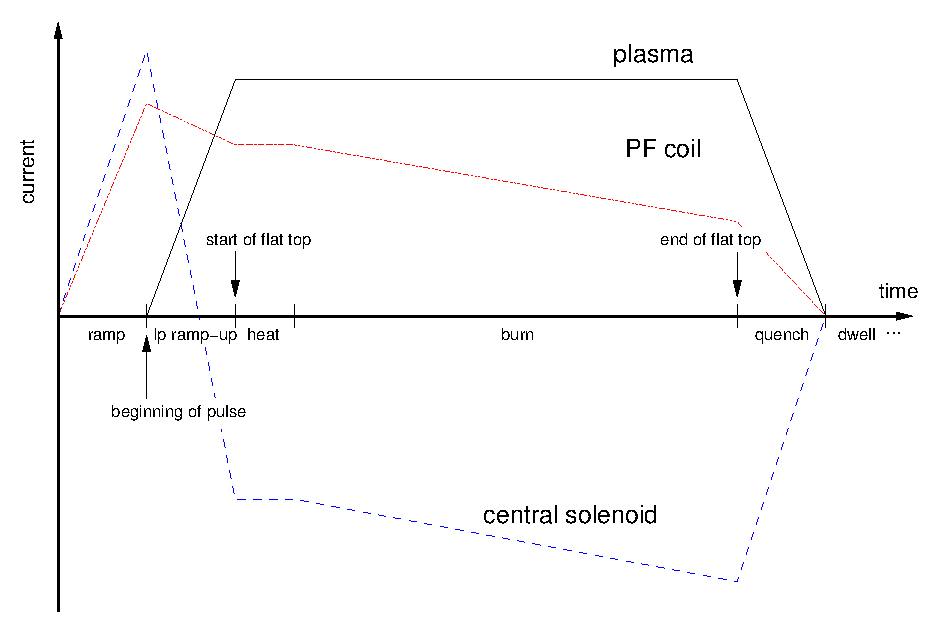
\epsfig{file=documentation/current_vs_time.eps,width=170mm}
\caption[Coil and plasma current waveforms]
{\label{fig:current_vs_time}
  \textit{Plot showing schematically the current waveforms for the plasma, a
    typical PF coil, and the central solenoid. Note that the currents in some
    of the PF coils may be the opposite sign to that shown, and the central
    solenoid current may remain positive during the $I_p$ ramp-up period,
    although it will pass through zero during the burn phase.}
}
\end{figure}

\subsubsection{PF coil material}

The PF coils can be either resistive or superconducting. This is determined
from the value of \texttt{ipfres}. If \texttt{ipfres = 0}, the PF coils and
the central solenoid are assumed to be superconducting. If \texttt{ipfres = 1},
they are assumed to be resistive, with their resistivity given by the value of
variable \texttt{pfclres}.

If \texttt{ipfres = 0}, switch \texttt{isumatpf} specifies which
superconducting material is to be used for the PF coils. The values for
\texttt{isumatpf} are used in the same way as switch \texttt{isumattf} is for
the TF coils (see Section~\ref{sec:superconductors}).

The fraction of copper present in the superconducting filaments is given by
the value of variable \texttt{fcupfsu}.

If the PF coils are superconducting, a steel case is assumed to surround the
current-carrying winding pack to take the hoop stress. Its cross-sectional
area is determined by the $J \times B$ hoop force on the coil divided by the
allowable hoop stress, given by input parameter \texttt{sigpfcalw}. The input
parameter \texttt{sigpfcf} provides a scale factor (default is 0.666) to
adjust the hoop force if required, to indicate what proportion of the force is
supported by the case.

\subsection{Central solenoid}
\label{sec:ohcoil}

Formerly known as the ohmic heating (OH) coil, the central solenoid is a PF
coil used during start-up and during the burn phase to create
and maintain the plasma current by inductive means. Swinging (changing) the
current through the central solenoid causes a change in the flux linked to the
plasma region, inducing a current in it. \process\ calculates the amount of
flux required to produce the plasma current, and also the amount actually
available. The code measures the magnetic flux in units of Volt-seconds ($=$
Webers).

Switch \texttt{iohcl} controls whether a central solenoid is present. A value
of \texttt{1} denotes that this coil is present, and should be assigned a
non-zero thickness \texttt{ohcth}. A value of \texttt{iohcl = 0} denotes that
no central solenoid is present, in which case the thickness \texttt{ohcth}
should be set to zero. No PF coils should be located at positions defined by
\texttt{ipfloc(j) = 1} if no central solenoid is present.

The central solenoid can be either resistive or superconducting (controlled
via switch \texttt{ipfres} as for the other PF coils), and if superconducting,
switch \texttt{isumatoh} determines the superconducting material to use ---
its value is used like \texttt{isumattf} and \texttt{isumatpf}. The fraction
of copper present in the superconducting filaments is given by the value of
variable \texttt{fcuohsu}.

If the central solenoid is superconducting, the coil contains steel for
strength. The cross-sectional area of steel is determined by the $J \times B$
hoop force on the coil divided by the allowable hoop stress, given by the input \texttt{alstroh}. A steel
thickness is given in the output, which would be the thickness of a
steel case of the same cross-sectional area if it simply surrounded the
conducting region.

\subsubsection{Current density inputs and limits}

The (absolute value of the) central solenoid current density at the
end-of-flat-top (`EOF'), \texttt{coheof} is specified by the user, and can be
used as an iteration variable (no.\ 37). The current density at the
beginning-of-pulse (`BOP' --- see Figure~\ref{fig:current_vs_time}) is
specified as a (positive) fraction of \texttt{coheof} using \texttt{fcohbop}
(iteration variable no.\ 41). The current density in the CS at all other times
is calculated by taking account of the flux swing necessary to initiate and
maintain the plasma current. The positive or negative sign of the current at
each time is calculated automatically.

The current density in the central solenoid can be limited at the BOP and at
the EOF. To limit the current density at the BOP, constraint equation no.\ 27
should be turned on with iteration variable no.\ 39 (\texttt{fjohc0}). To
limit the current density at the EOF, constraint equation no.\ 26 should be
turned on with iteration variable no.\ 38 (\texttt{fjohc}).

As for the TF coils, the critical current density \jcrit\ falls with the
temperature of the superconductor. The temperature margin $\Delta T$ is the
difference between the temperature at which \jcrit would be equal to \jop\ and
the operating temperature. The minimum allowed $\Delta T$ can be set using
input parameter \texttt{tmargmin} together with constraint equation no.\ 60
and iteration variable no.\ 106 (\texttt{ftmargoh}).

Note that if the temperature margin is positive, \jop\ is guaranteed to be
lower than \jcrit, and so constraints~26, 27 and~60 need not all be turned on
(in fact, it is recommended that EITHER the latter constraint, OR the former
two constraints, is/are activated in any given run).

\subsubsection{Plasma current ramp-up time}
\label{sec:tohs}

In the steady-state power plant scenario ($\mathtt{lpulse \not= 1}$ --- see
Section~\ref{sec:pulsed}), the length of time taken for the central solenoid
current to (possibly) reverse (which is equal to the plasma current ramp-up time --- see
Figure~\ref{fig:current_vs_time}) is determined from the value of switch
\texttt{tohsin}. If \texttt{tohsin = 0}, then the plasma current ramp-up
time \texttt{tohs} in seconds is given by $\mathtt{tohs} = I_p / 0.5$, where
$I_p$ is the plasma current in MA\@. Furthermore, the PF coil ramp time
\texttt{tramp} and shutdown time \texttt{tqnch} are set equal to
\texttt{tohs}.  If $\mathtt{tohsin \not= 0}$, the plasma current ramp-up
time \texttt{tohs = tohsin}, and the PF coil ramp and shutdown times are input
parameters.

If, however, a pulsed power plant is being modelled (\texttt{lpulse = 1}), the
plasma current ramp-up time \texttt{tohs} is either an input parameter, or it can be
iterated by using iteration variable~65. The ramp and shutdown times in the
pulsed case are always set equal to \texttt{tohs}. To ensure that the plasma
current ramp rate during start-up is prevented from being too high, as
governed by the requirement to maintain plasma stability by ensuring that the induced current has time to diffuse into the body of the plasma, constraint equation no.\ 41 should be turned on with iteration variable no.\ 66 (\texttt{ftohs}).

\subsection{Auxiliary power systems: heating and current drive}
\label{sec:hcd}

\subsubsection{Current Drive}

The use of inductive current drive leads to pulsed plant operation
because of the limited flux swing that can be achieved using the central
solenoid. This poses problems due to the fact that fatigue failures may
result, and there would also be a need for thermal storage to maintain output of electricity
between pulses, and supply power for starting a new pulse. However, the plasma current can also be produced and
maintained (partially or wholly) using non-inductive means which, in
principle, removes this restriction. \process\ contains a number of auxiliary
current drive schemes, including various RF methods (Lower Hybrid, Electron
Cyclotron, and Ion Cyclotron (Fast Wave) current drives) and also Neutral Beam
current drive systems. The code calculates the efficiency and the resulting
power requirements of the chosen system.

The fraction of the required plasma current to be produced by non-inductive
means, \texttt{fvsbrnni}, should be set, and flag \texttt{irfcd} should be set
to \texttt{0} for purely inductive scenarios, or \texttt{1} otherwise. The
current drive efficiency model to be used in this latter case is defined by
the value of switch \texttt{iefrf}:-
\begin{description}
\item [\texttt{iefrf = 1} :] Fenstermacher Lower Hybrid model
\item [\texttt{iefrf = 2} :] Ion cyclotron model~\cite{IPDG}
\item [\texttt{iefrf = 3} :] Fenstermacher electron cyclotron resonance model
\item [\texttt{iefrf = 4} :] Ehst Lower Hybrid model
\item [\texttt{iefrf = 5} :] ITER neutral beam model~\cite{IPDG,172}
\item [\texttt{iefrf = 6} :] Culham Lower Hybrid model~\cite{172}
\item [\texttt{iefrf = 7} :] Culham electron cyclotron model~\cite{172}
\item [\texttt{iefrf = 8} :] Culham neutral beam model~\cite{172}
\item [\texttt{iefrf = 9} :] Oscillating Field current drive (RFPs only - OBSOLETE)
\end{description}

(Note that, at present, the neutral beam models do not include the effect of an edge transport barrier (pedestal) in the plasma profile.)

It is sometimes useful to adjust artificially the current drive efficiency
values produced by these routines. This can be achieved by setting the scaling
coefficient \texttt{feffcd}. The wall plug to plasma efficiencies can also be
adjusted, by changing the relevant variable (\texttt{etaech}, \texttt{etalh},
\texttt{etanbi} or \texttt{etaof}).

\subsubsection{Plasma heating}

In addition to current drive, some auxiliary power can be used purely to heat
the plasma. The value of input parameter \texttt{pheat} determines the amount
of auxiliary \textit{heating}\/ power (in Watts) to be applied to the
plasma. This variable may be used as an iteration variable (no.\ 11).

\subsubsection{Neutral beam access}

If present, a neutral beam injection system needs sufficient space between the
TF coils to be able to intercept the plasma tangentially. The major radius
\texttt{rtanbeam} at which the centreline of the beam is tangential to the
toroidal direction is user-defined using input parameter \texttt{frbeam},
which is the ratio of \texttt{rtanbeam} to the plasma major radius
\texttt{rmajor}. The maximum possible tangency radius \texttt{rtanmax} is
determined by the geometry of the TF coils --- see Figure~\ref{fig:portsize},
and this can be enforced using constraint equation no.\ 20 with iteration
variable no.\ 33 (\texttt{fportsz}). The thickness of the beam duct walls may
be set using input parameter \texttt{nbshield}.

\begin{figure}[tbph]
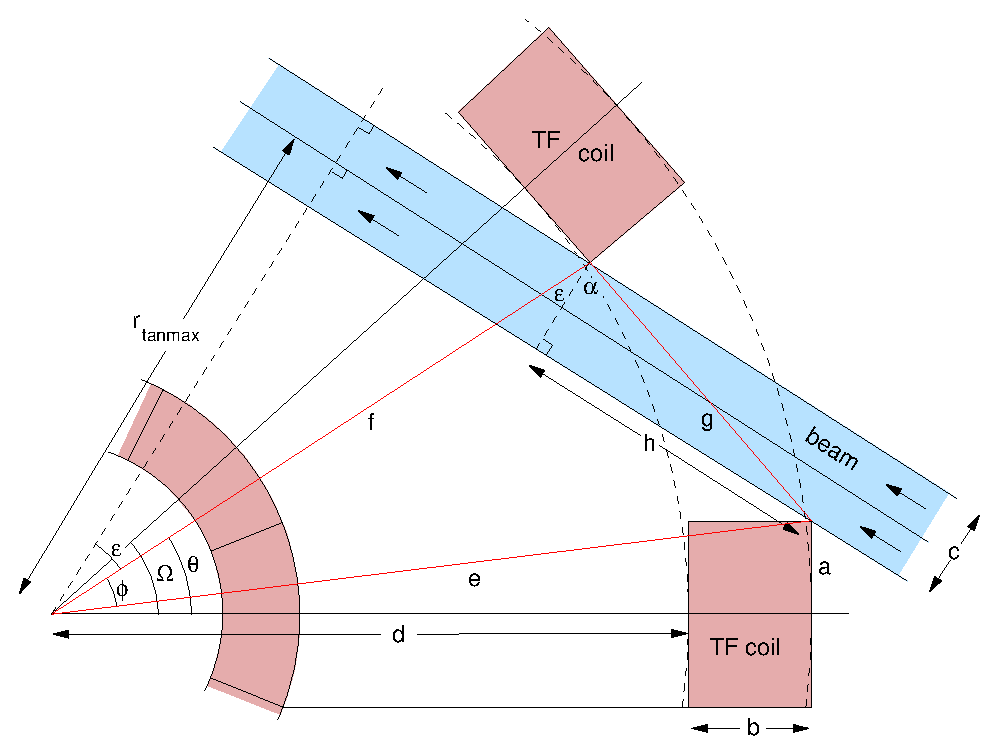
\epsfig{file=documentation/portsize.eps,width=160mm}
\caption[Schematic diagram of the neutral beam access geometry]
{\label{fig:portsize}
  \textit{Top-down schematic view of the neutral beam access geometry. The beam
    with the maximum possible tangency radius is shown here.}
}
\end{figure}

\subsubsection{Neutral beam losses}

Input parameter \texttt{forbitloss} can be used to specify the fraction of the
net injected neutral beam power that is lost between the beam particles'
ionisation and thermalisation (known as the first orbit loss). This quantity cannot easily be calculated as it depends on the field ripple and other three-dimensional effects.  The power lost
is assumed to be absorbed by the first wall.

The power in the beam atoms that are not ionised as they pass through the plasma (shine-through) is calculated by the code.  There are two constraint equations that can be used to control the beam
penetration and deposition, as follows:
\begin{itemize}

\item It is necessary to use a beam energy that simultaneously gives adequate
  penetration of the beam to the centre of the plasma and tolerable
  shine-through of the beam on the wall after the beam has traversed the
  plasma. The number of exponential decay lengths, $\tau$, for the beam power
  to fall before it reaches the plasma centre should be in the region of $\sim
  4$--6~\cite[Section 4.3.2]{172}. Constraint equation no.\ 14 may be used to
  force $\tau$ to be equal to the value given by input parameter
  \texttt{tbeamin}, and is therefore in effect a beam energy consistency
  equation.

\item Alternatively, constraint equation no.\ 59 with iteration variable no.\
  105 (\texttt{fnbshinef}) may be used to ensure that the beam power fraction
  emerging from the plasma is no more than the value given by input parameter
  \texttt{nbshinefmax}.

\end{itemize}

It is recommended that \textbf{only one} of these two constraint equations is
used during a run.

\subsubsection{Ignited plasma}
\label{sec:ignited}

Switch \texttt{ignite} can be used to denote whether the plasma is ignited,
i.e.\ fully self-sustaining without the need for any injected auxiliary power
during the burn. If \texttt{ignite = 1}, the calculated injected power does
not contribute to the plasma power balance (Section~\ref{sec:corepower}),
although the cost of the auxiliary power system is taken into account (the
system is then assumed to be required to provide heating etc.\ during the
plasma start-up phase only --- use \texttt{pheat} to indicate the power
requirement). If \texttt{ignite = 0}, the plasma is not ignited, and the
auxiliary power is taken into account in the plasma power balance during the
burn phase. Also, constraint equation no.\ 28 can be turned on to enforce the
fusion gain $Q$ to be at least \texttt{bigqmin}.

\subsection{Structural components}

Structural components are required to provide support for the fusion power
core systems against gravity and the magnetic forces that will be encountered
during operation. The required structural masses and their costs are
calculated.

\subsection{Cryostat and vacuum system}

The internal vacuum vessel provides a toroidal evacuated chamber containing
the plasma, first wall, blanket and shield, and the space between this item
and the external cylindrical cryostat encloses those components that need to
operate at liquid helium temperatures. These include any superconducting (TF
or PF) coils and the inter-coil structure. \process\ calculates the cryogenic
power load and the resulting heat exchanger requirements.

The vertical distance \textit{h}\/ between the uppermost PF coil and the
external cryostat lid may be adjusted by changing the value of input parameter
\texttt{clhsf}; a scaling based on ITER is used:
\begin{equation}
h = \mathtt{clhsf} \, \left( \frac{2 \times \mathtt{rdewex}}{28.440} \right)
\end{equation}

The vacuum system is used for four different processes. Firstly, before plasma
operations the chamber must be evacuated to remove outgassed impurities from
the structure. Secondly, the chamber must be re-evacuated between burn
operations. Thirdly, helium ash must be removed to prevent it from diluting
the fuel. Finally, deuterium and tritium is removed on a steady state
basis. \process\ calculates the parameters of a vacuum system that satisfy
all four requirements, with the option of either turbo pumps or cryo pumps
being used.

Switch \texttt{ntype} controls whether a turbopump (\texttt{ntype = 0}) or a
cryopump (\texttt{ntype = 1}) is used in the vacuum system.

\subsection{Power conversion and heat dissipation systems}
\label{sec:powerflow}

The \process\ power plant takes into account all the systems required to
perform the necessary conversion of fusion power to electricity, from the
coolant systems in the plant components to the heat exchangers and turbines.

Figure~\ref{fig:powerflow3} shows the overall power transfer mechanisms within the power plant outside of the plasma.  The efficiency of the primary coolant pumps in converting electrical to mechanical power is given by input parameter \texttt{etahtp} in all the calculations described below.

%\begin{figure}[tbph]
%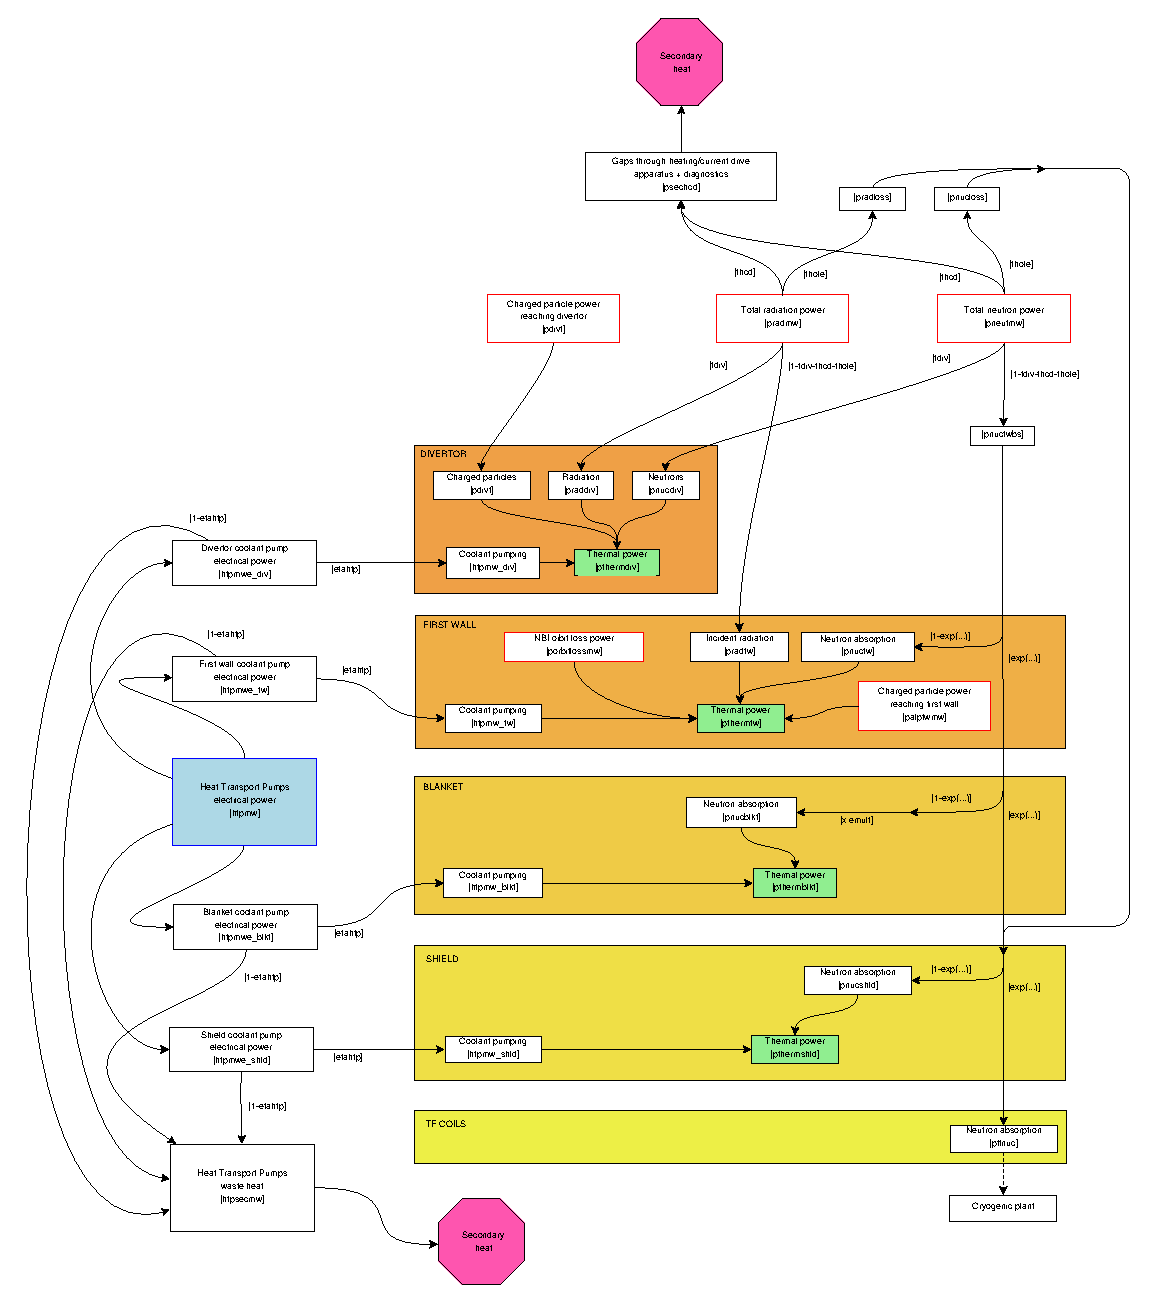
\epsfig{file=powerflow2.eps,width=170mm}
%\caption[Power flow within the fusion power plant core]
%{\label{fig:powerflow2} \textit{Schematic diagram of the flow of power from
%    the plasma to the thermal power deposited within the divertor, first wall,
%    blanket and shield. Variable names are given in [\ldots]. The five
%    red-bordered contributions are passed from Figure~\ref{fig:powerflow1},
%    while the blue box comes from Figure~\ref{fig:powerflow3}.} }
%\end{figure}

\subsubsection{Divertor}
\label{sec:divpower}

All of the charged particle transport power leaving the plasma (excluding the
\texttt{1-falpha} portion of the alpha power that escapes directly to the first
wall --- Section~\ref{sec:corepower}) is assumed to be absorbed in the
divertor, along with a proportion \texttt{fdiv} of the radiation power and the
neutron power. 

Switch \texttt{iprimdiv} may be used to specify whether the thermal power
deposited in the divertor becomes high-grade thermal power
(\texttt{iprimdiv = 1}) or low-grade waste heat (see
Figure~\ref{fig:powerflow3}). 
%(N.B.\ see also the caption for Table~\ref{tab:etath}.)

\subsubsection{First wall}

The remaining photon power (i.e.\ the fraction not incident upon the divertor or lost through holes or the heating / current drive apparatus) is assumed to be absorbed by the first wall. Power due to ions derived from the neutral beams but lost before being thermalised (known as "first orbit loss"), and from the fast alpha particles lost before being thermalised, also contribute to the total thermal power absorbed by the first wall.

\subsubsection{Thermal cycling package}
This performs calculations on the first wall of the machine. Evaluation of the
mechanical and thermal stresses on this component lead to a measure of the
maximum number of cycles to which the first wall can be subjected, and hence
to the minimum allowable length of each reactor cycle for a specified first
wall lifetime. The cycle time can be constrained to be at least the minimum
value by turning on constraint equation no.\ 42 with iteration variable no.\
67 (\texttt{ftcycl}).

The thickness of the first wall is constrained to lie within lower and upper
bounds, which ensures that it can withstand the internal coolant pressure and
the peak temperature and neutron fluence.

Switch \texttt{itcycl} activates the desired model for the first wall axial
stress calculations. If \texttt{itcycl = 1} (the default), the wall is fully
constrained axially, and no bending can occur. If \texttt{itcycl = 2}, there
is no constraint on the axial motion, but no bending can occur. Finally, if
\texttt{itcycl = 3}, again there is no axial constraint, and bending is
allowed to occur.

\subsubsection{First wall coolant temperature rise limit}

The rise in temperature of the first wall coolant can be limited to be no more
than the value of \texttt{dtmpmx} by turning on constraint equation no.\ 38 with
iteration variable no.\ 62 (\texttt{fdtmp}).

\subsubsection{First wall peak temperature limit}

The maximum first wall temperature can be limited to be no more than the value
of variable \texttt{tpkmax} by turning on constraint equation no.\ 39 with
iteration variable no.\ 63 (\texttt{ftpeak}).


\subsubsection{Power conversion cycle}
\label{sec:etath}

Figure~\ref{fig:powerflow3} summarises the power conversion mechanisms.

\begin{figure}[tbph]
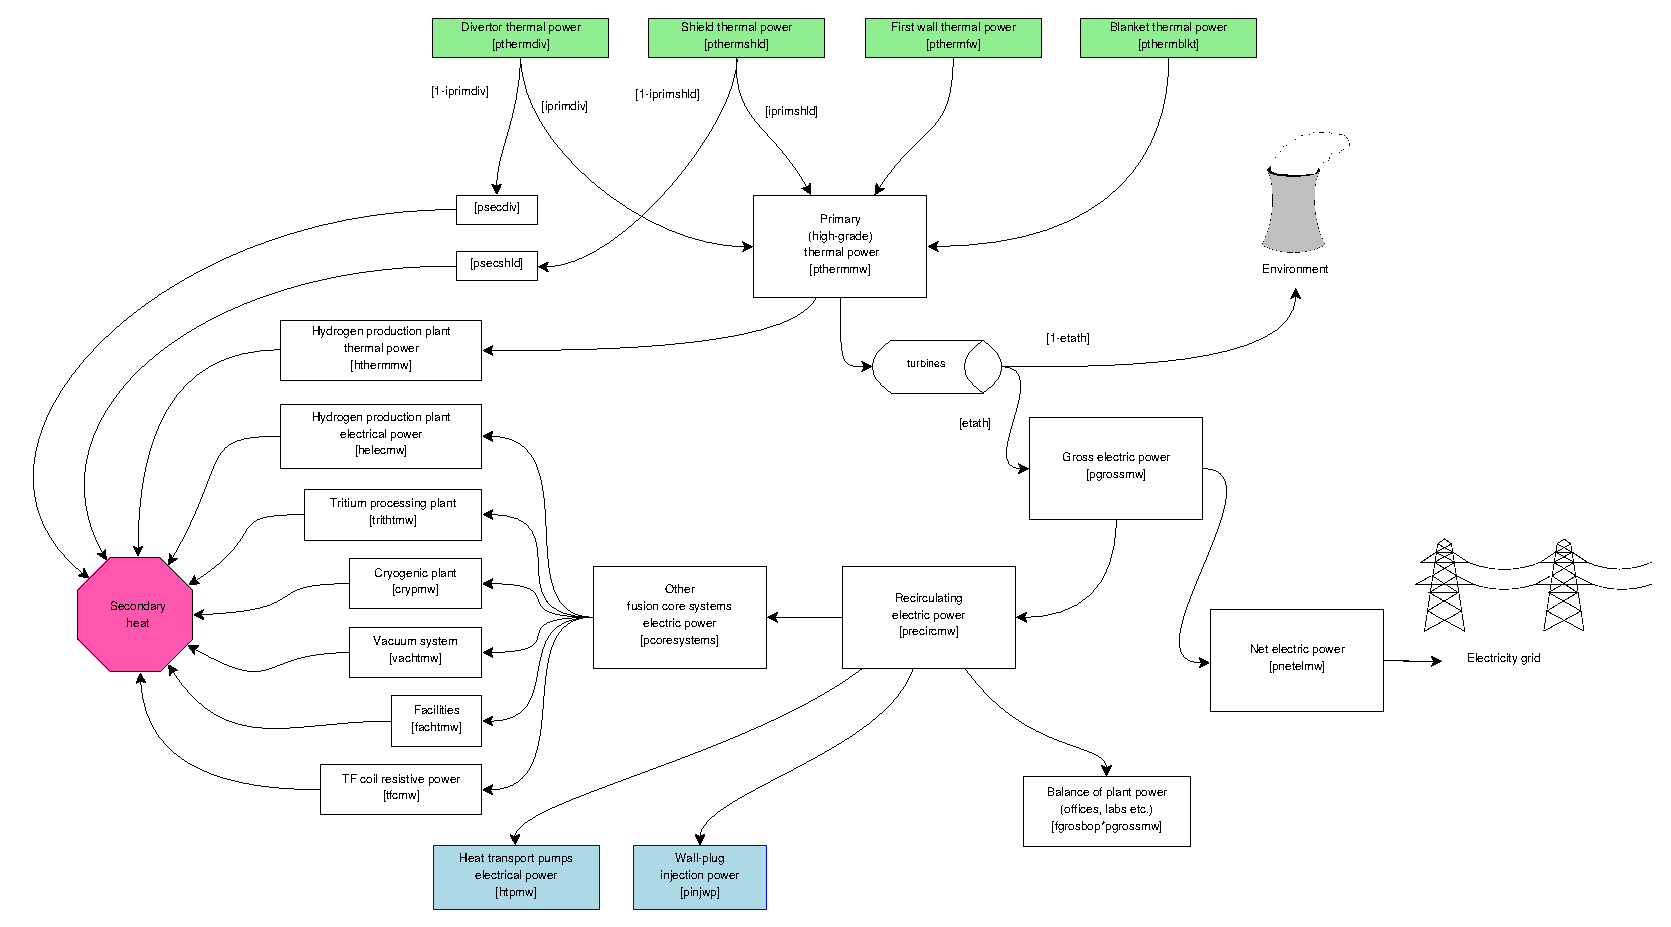
\epsfig{file=documentation/powerflow3.eps,width=170mm}
\caption[Power flow outside the fusion power plant core]
{\label{fig:powerflow3} \textit{Schematic diagram of the flow of power beyond
    the fusion power core, showing the origin of the high-grade and waste
    heat and the electrical power balance within the plant. Variable
    names are given in [\ldots]. The input power contributions in green boxes
    originate in Figure~\ref{fig:powerflow1}. }  }
\end{figure}

The high-grade, i.e.\ useable thermal power (less any thermal power required to
produce hydrogen in a hydrogen production plant --- see
Section~\ref{sec:hplant}) is used to produce steam to turn the turbines, thus
generating the plant's gross electrical power, with an efficiency given by
quantity \texttt{etath}. The remainder is dumped to the environment through the condenser.  All of the low-grade heat is dumped to the environment.

\begin{description}
\item{\texttt{primary\_pumping }:} This switch controls the calculation of the mechanical pumping power required for the primary coolant.

If \texttt{primary\_pumping = 0}, the user sets mechanical pumping power directly.

If \texttt{primary\_pumping = 1}, the user sets mechanical pumping power as a fraction of thermal power removed by coolant.

If \texttt{primary\_pumping = 1}, the mechanical pumping power is calculated, as follows.

User inputs for the coolant outlet temperature (which may be used as an iteration variable), the coolant channel diameter, and the segmentation of the blanket are used.  The peak temperature in the first wall material (underneath the armour) is derived. The user can apply an upper limit to this temperature, and if this constraint is used then it is strongly recommended to set the length of a first wall pipe (\texttt{fw\_channel\_length})as an iteration variable. The Gnielinski correlation is used to determine the heat transfer in the channel.  The stresses in the first wall are not currently taken into account. 

The mechanical pumping power required for the first wall and breeder zone is calculated using the Darcy friction factor, estimated from the Haaland equation, an approximation to the Colebrook–White equation. (If you consider that the calculated value for the pumping power is too low, then you can add an additional electric power requirement using \texttt{baseel}.  Do not use \texttt{htpmw\_min} as this prevents the optimisation of the first wall.) The inlet and outlet temperatures of the first wall and blanket can be different. The isentropic efficiency of the first wall and blanket coolant pumps (enthalpy increase in the fluid for isentropic compression divided by the mechanical power used) is specified by the parameter \texttt{etaiso}.  Note that the mechanical pumping powers for the shield and divertor are still calculated using the simplified method (a fixed fraction of the heat transported). 

\end{description}

\begin{description}
\item{\texttt{secondary\_cycle }:} This switch controls how the calculation of the plant's thermal to electric conversion efficiency (the secondary cycle thermal efficiency) proceeds. See also Section~\ref{sec:powerflow}, which describes the flow of power through the fusion power core.

If \texttt{secondary\_cycle = 0}, the efficiency of the power generation cycle is set to a single value obtained from previous cycle modelling studies.  The heat deposited in theToroidal field coils divertor coolant is assumed to be at such low temperature that it cannot be used for power generation and is dumped to the environment.

If \texttt{secondary\_cycle = 1}, the efficiency of the power generation cycle is set as above, but the divertor heat is used for electricity generation.

In the remaining options (\texttt{secondary\_cycle = 1, 2 or 3}), the heat deposited in the divertor coolant is used for power generation.

If \texttt{secondary\_cycle = 2}, the efficiency of the power generation cycle is input by the user.

If \texttt{secondary\_cycle = 3}, a steam Rankine cycle is assumed.  The secondary cycle thermal efficiency (\texttt{etath}) is calculated from the coolant outlet temperature using simple relations between temperature and efficiency ~\cite{Harrington_bop}:
\begin{eqnarray}
\eta & = & -2.0219 + 0.3720 \, \ln(T) \;\;\; \mbox{\small(water coolant;
  saturated steam Rankine cycle)} \\
\eta & = & -0.8002 + 0.1802 \, \ln(T) \;\;\; \mbox{\small(helium coolant;
  superheated steam Rankine cycle)}
\end{eqnarray}

If \texttt{secondary\_cycle = 4}, a supercritical CO$_2$ Brayton cycle is assumed.  The secondary cycle thermal efficiency (\texttt{etath}) is calculated from the coolant outlet temperature using simple relations between temperature and efficiency from ~\cite{Harrington_bop}:
\begin{equation}
\eta = -2.5043 + 0.4347 \, \log(T) \;\;\; \mbox{\small(water or
  helium coolant}
\end{equation}
  
\end{description}


%Table~\ref{tab:etath} summarises these options.

% Table summarising the etath calculation
% The WCLL and HCLL options are not yet available, so I have commented this table out for the moment.

%\begin{table}[tbph]
%\begin{center}

%\begin{tabular}{||l||c||c||c||} \hline
% & \texttt{blkttype = 1} & \texttt{blkttype = 2} & \texttt{blkttype = 3} \\
% & WCLL & HCLL & HCPB \\ \hline
%Divertor heat $\longrightarrow$ primary power & 31.11\%  & 39.70\% & 39.70\% \\
%\texttt{iprimdiv = 1} & & & \\ \hline
%Divertor heat $\longrightarrow$ secondary power & --- & 43.60\% & 43.60\% \\
%\texttt{iprimdiv = 0} & & & \\ \hline
%\end{tabular}
%\end{center}
%\caption[Summary of plant thermal to electric conversion efficiency values]
%{\label{tab:etath}
%  \textit{Summary of the plant thermal to electric conversion efficiency
%    values, \texttt{etath}, for \texttt{blktcycle=0}. Note that the WCLL
%    modelling on which the figures are based assumed that the divertor heat
%    was used in the primary cycle, so switch \texttt{iprimdiv=1} is enforced
%    if \texttt{blktcycle=0} and \texttt{blkttype=1}.}
%}
%\end{table}

In the above three equations, $T$ is the temperature of the (secondary)
coolant at the inlet to the turbine, assumed to be a fixed margin below the
outlet temperature of the primary coolant.

The electrical power required to operate the power plant itself is the
so-called recirculating electric power. Any surplus is exported to the
electricity grid as net electric power.

The recirculating power comprises the electrical power required to run all of
the associated electrical systems surrounding the fusion power core, plus the
on-site building services, offices, etc., as shown in
Figure~\ref{fig:powerflow3}. Of these, the cryogenic plant power includes the
power required to cool the TF coils from the neutron power absorbed by the
coils, the PF coils (as defined by the ratio of the total PF coil stored
energy to the fusion power pulse time \texttt{tpulse}), and other `cold'
components.

\subsection{Buildings}

The volume and ground area of all the various buildings on a power plant site
are included in the \process\ calculations for the benefit of the costing
algorithms. %!%!%! expand

\section{Spherical Tokamak Model}
\label{sec:tart}

\process\ has the ability to perform studies on tokamaks in the low aspect ratio
regime (major radius $\leq 2 \times$ minor radius). The physics and
engineering issues~\cite{tart} associated with these machines are somewhat
different from those of conventional aspect ratio, and this is reflected by
the following special models~\cite{storac} in \process.
\begin{enumerate}

\item The inboard build of a spherical tokamak (ST) is very different from
  that in a conventional tokamak. There is no inboard blanket (and possibly no
  inboard shield), and the inboard TF coil legs are replaced by a single
  centrepost. The radial build is altered so that, starting from the
  centreline ($R = 0$), the component order is: TF coil, gap, central
  solenoid, vacuum vessel, and then continuing as in Figure~\ref{fig:build_d}
  (a D-shaped cross-section is assumed for the first wall, blanket, shield and
  vacuum vessel).

\item Spherical tokamaks have resistive TF coils that combine into a single
  centrepost at the centre of the machine. The centrepost is constructed from
  copper (as are the outboard TF coil sections), and is tapered lengthways so
  that it is narrowest at the midplane of the device.  Routine
  \texttt{CNTRPST} calculates various parameters relevant to the centrepost,
  including the pump pressure, maximum temperature and pipe radius, and these
  may be limited using constraint equations~43 to~46 if required:
  \begin{itemize}
  \item Equation~43 is a consistency equation for the average centrepost
    temperature.
  \item Equation~44 can be used to limit the peak centrepost temperature to a
    maximum value (\texttt{ptempalw}) using iteration variable no.\ 68
    (\texttt{fptemp}).
  \item Equation~45 can be used to force a lower limit to the edge safety
    factor $q_{lim}$ (see below), using iteration variable no.\ 71 (\texttt{fq}).
  \item Equation~46 can be used to apply an upper limit to the ratio of plasma
    current to TF coil (``rod'') current, using iteration variable no.\ 72
    (\texttt{fipir}).
  \end{itemize}

\item A gaseous divertor model is used, and a simple divertor heat load
  calculation is employed, rather than the more complex divertor model assumed
  for conventional aspect ratio tokamaks.

\item A simple PF coil current scaling algorithm is available for use with the
  ST option.

\item The plasma shaping terms (elongation and triangularity) can be
  calculated directly given the aspect ratio, using \texttt{ishape = 1} (see
  Section~\ref{sec:plasma_geometry}). This setting also scales the lower
  limit~\cite{storac} for the edge safety factor, for use with constraint
  equation no.\ 45:
  \begin{equation}
    q_{lim} = 3 \, (1 + 2.6*\epsilon^{2.8})
  \end{equation}
  where $\epsilon = a/R$. 

\item Among the physics models that differ from those relevant to conventional
  aspect ratio machines are (i) the plasma poloidal field $B_{pol}$, (ii) the
  bootstrap current fraction, (iii) the beta limit, and (iv) the neutron
  heating of the centrepost~\cite{storac}.

\end{enumerate}

\subsection{Spherical tokamak switches}

Switch \texttt{itart} provides overall control of the ST switches within the
code, and subroutine \texttt{CHECK} ensures that no conflicting values are
inadvertently set by the user in the input file. Table~\ref{tab:tart}
summarises the switch values relevant to each aspect ratio regime.

\begin{table}[tbph]
\begin{center}
  \begin{tabular}{||l|c|c||} \hline
    & conventional aspect ratio & low aspect ratio \\
    switch & \texttt{itart = 0} & \texttt{itart = 1} \\ \hline
    \texttt{ishape} (Section~\ref{sec:plasma_geometry}) & 0, 2 & 0, 1 \\
    \texttt{ibss} (Section~\ref{sec:bootstrap}) & 1, 2, 3 & 2, 3 \\
    \texttt{icurr} (Section~\ref{sec:current_scaling}) & 1, 3, 4, 5, 6, 7 & 2 \\
    \texttt{itfsup} (Section~\ref{sec:tfcoil}) & 0, 1 & 0 \\
    \hline
\end{tabular}
\end{center}
\caption[\process\ switches for spherical tokamaks]
{\label{tab:tart}
  \textit{Summary of the switch values in PROCESS that relate to
    conventional aspect ratio and low aspect ratio machines.}
}
\end{table}

\section{Pulsed Plant Operation}
\label{sec:pulsed}

If the plasma current is partially or entirely driven by electromagnetic induction, it is
necessary to operate the plant in a pulsed manner as the current swing in the
central solenoid coils cannot be continued indefinitely. \process\ can perform a number of
calculations relevant to a pulsed power plant, as detailed below.

Switch \texttt{lpulse} determines whether the power plant is assumed to be
based on steady-state (\texttt{lpulse = 0}) or pulsed (\texttt{lpulse = 1})
operation.

\subsection{Start-up power requirements}

The minimum auxiliary power required during the start-up (ignition) phase is
calculated on the basis of a POPCON analysis. Ignition is accessed via the
so-called Cordey Pass (the path in plasma density--temperature space which
minimises the power requirement) and the code ensures that there is sufficient
auxiliary power to accommodate this. In fact, this calculation is very
CPU-intensive, so the relevant routine is not called at present. In practice,
the auxiliary power tends to exceed the minimum allowable value anyway,
without any need to constrain it to do so.

The auxiliary power reaching the plasma can be forced to be more than the
minimum allowable value \texttt{auxmin} by turning on constraint equation no.\
40 with iteration variable no.\ 64 (\texttt{fauxmn}). The value of
\texttt{auxmin} is determined by the code if the start-up model is activated,
otherwise it may be initialised via the input file.

\subsection{Plasma current ramp-up time}

This calculation ensures that the plasma current ramp rate during start-up is
prevented from being too high, as governed by the requirement to maintain
plasma stability in $l_i$ - $q_\psi$ space (see Section~\ref{sec:tohs}).

\subsection{Burn time}

The length of the burn time is calculated from the surplus volt-seconds
available from the OH/PF coil system during the plasma burn phase, after the
flux required during the plasma start-up is taken into account. A minimum burn
time can be enforced via constraint equation no.\ 13 and iteration variable
no.\ 21 (\texttt{ftburn}).

\subsection{Thermal storage}

During every cycle there is a period when no fusion power is produced. The net
electric output from the plant must, however, be maintained, and this is
achieved using thermal storage. There are three types of thermal storage
available within \process, and the value of switch \texttt{istore} determines
which is to be used. If \texttt{istore = 1} (the default), option~1 of
Ref.~\cite{ELECTROWATT} is assumed, which utilises the thermal storage
inherent in the machine's steam cycle equipment. This should be used if the
machine down time is less than 100~seconds. If \texttt{istore = 2}, option~2
of Ref.~\cite{ELECTROWATT} is assumed, which uses the same method as before,
but augments it with an additional boiler. This may be used for machine down
times of up to 300~seconds. Finally, if \texttt{istore = 3}, a large stainless
steel block acts as the thermal storage medium.

\section{Hydrogen Production Facility}
\label{sec:hplant}

Fusion power plants have been mooted as a means of producing hydrogen for use
in fuel cells for cars, for instance. \process\ includes options to enable
the plant to produce hydrogen using a number of different processes.

To include the production of hydrogen by the power plant, it is necessary to
set the switch \texttt{ihplant}, as follows:
\begin{description}
\item [\texttt{ihplant = 0} :] No hydrogen production (default)
\item [\texttt{ihplant = 1} :] Hydrogen production by low temperature electrolysis
\item [\texttt{ihplant = 2} :] Hydrogen production by endothermic high
  temperature electrolysis
\item [\texttt{ihplant = 3} :] Hydrogen production by exothermic high
  temperature electrolysis
\item [\texttt{ihplant = 4} :] Hydrogen production by thermo-chemical processes
\end{description}
Table~\ref{tab:hplant} describes the additional options available for each of
the types of hydrogen production given above. The different processes use
either electrical power or thermal power directly, so the required inputs
differ. Variable \texttt{helecmw} (iteration variable no.\ 87) is the
electrical power in MW required for hydrogen production, while
\texttt{hthermmw} (iteration variable no.\ 88) is the thermal power
required. Note that \texttt{hthermmw} must not be used as an iteration
variable if $\mathtt{ihplant \not= 4}$, as it will be calculated from the
required electrical power instead. Similarly, \texttt{helecmw} must not be
used as an iteration variable if \texttt{ihplant = 4}.

\begin{table}[tbph]
\begin{center}
\begin{tabular}{||c|c|c|c||} \hline
hydrogen plant option & \texttt{helecmw} & \texttt{hthermmw} & efficiency
variable \\ \hline
\texttt{ihplant=1} & input & zero & \texttt{etahlte} \\
\texttt{ihplant=2} & input & calculated & \texttt{etahten} \\
\texttt{ihplant=3} & input & calculated & \texttt{etahtex} \\
\texttt{ihplant=4} & zero & input & \texttt{etahth} \\
\hline
\end{tabular}
\end{center}
\caption[Variables used in the hydrogen plant model]
{\label{tab:hplant}
  \textit{Summary of the variables in PROCESS that relate to
    the different hydrogen plant processes.}
}
\end{table}
The efficiency variables given in Table~\ref{tab:hplant} are all input
parameters, and are the factors to be used to convert the value of
\texttt{helecmw} to the amount of hydrogen produced (in MW equivalent); these
can be greater than unity in all cases except \texttt{ihplant = 4}.

\section{Stellarator Model}

The code has the ability to perform calculations based on the physics and
engineering of a stellarator, which, although being a toroidal device, is
radically different in a number of ways from a tokamak.

The model is largely based on W7-X and the HELIAS 5-B stellarator power plant
design~\cite{helias5b} (Figure~\ref{fig:helias5b}) and related modelling that
has been performed by IPP Greifswald~\cite{stell_geometry, stell_divertor,
  stell_coil}.

To activate the stellarator coding, it is necessary to create a file
\texttt{device.dat}, containing the single character \texttt{1} in the first
row, in the working directory (see Section~\ref{sec:infile}). This has the
effect of setting the internally-used switch \texttt{istell = 1}. If the file
is absent, or its first character is set to something other than \texttt{1},
the stellarator model is not used, and \texttt{istell} is set to
\texttt{0}.

The stellarator model is largely contained within source file
\texttt{stellarator.f90}. The following consistency equations (see
Section~\ref{sec:constraints}) should be used without modification:
\begin{description}
\item [\texttt{1} :] plasma beta consistency
\item [\texttt{2} :] global power balance
\item [\texttt{11} :] radial build consistency
\end{description}

\begin{figure}[tbph]
\centerline{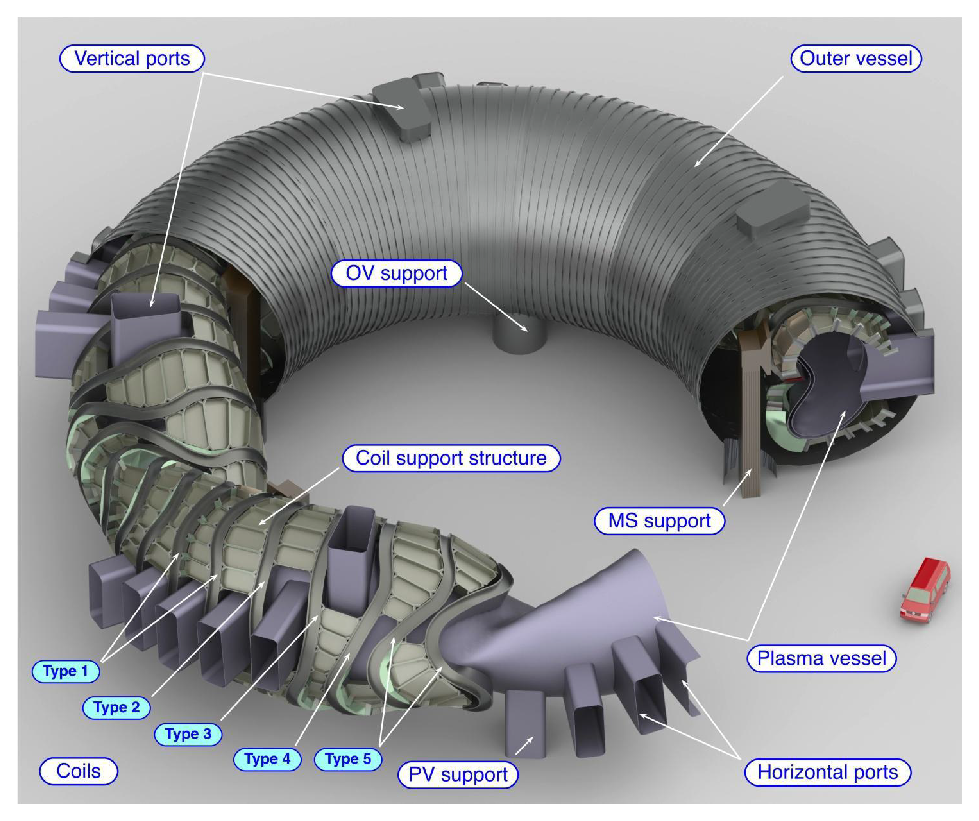
\epsfig{file=documentation/helias5b.eps,width=160mm}}
\caption[HELIAS 5-B Stellarator Power Plant Design]
{\label{fig:helias5b}
  \textit{Fusion power core of the HELIAS 5-B conceptual power plant design
    (from~\cite{helias5b})}
}
\end{figure}

\subsection{Stellarator physics}

Much of the physics is identical to that for tokamaks, including the plasma
composition and the fusion power calculations. However, some physics topics do
differ between stellarators and tokamaks, as follows.

\subsubsection{Plasma geometry}

The plasma geometry model uses Fourier coefficients to represent the complex
3-D plasma shape typical of stellarators. A VMEC~\cite{vmec} calculation (or
other equilibrium code that can provide the Fourier coefficients of the LCFS)
must have been performed prior to running with \process. The overall size of
the plasma is scaled correctly for the required (mean) major and minor radii
for the machine being modelled~\cite{geiger}.

It is necessary to provide three input files that define the plasma shape:
\begin{enumerate}

\item Set \texttt{vmec\_info\_file} in the input file to the name of a file
  with the following format (the numbers given are those for the W7-X high
  mirror configuration); in practice only the effective major and minor radius
  values (\texttt{R\_eff} and \texttt{a\_eff}, respectively) and the number of
  field periods are used:

\footnotesize
\begin{verbatim}
R_eff [m]   a_eff [m]   Aspect ratio   Plasma vol [m3]  LCFS surf area [m2]  field periods
5.486576    0.4942638   11.10050       26.45749         133.4281             5.0
\end{verbatim}
\normalsize

\item Set \texttt{vmec\_rmn\_file} in the input file to the name of a VMEC
  output file containing the calculated plasma boundary $R(m,n)$ Fourier
  coefficients, where $m = 0$ to 11 (rows) and $n = -12$ to 12 (columns).

\item Set \texttt{vmec\_zmn\_file} in the input file to the name of a VMEC
  output file containing the calculated plasma boundary $Z(m,n)$ Fourier
  coefficients, where $m = 0$ to 11 (rows) and $n = -12$ to 12 (columns).

\end{enumerate}

This method enables a wide range of potential plasma geometries to be
modelled, if required. The plasma volume, surface area and mean
cross-sectional area are the outputs from the plasma geometry model.

\subsubsection{Absense of plasma current}

Stellarators try to achieve zero plasma current in order to allow safe
divertor operation, so no current scalings are required.

\subsubsection{Beta limit}

The beta limit is assumed to be 5\%, based on 3-D MHD calculations
\cite{Nuhrenberg}. To apply the beta limit, constraint equation no.\ 24 should
be turned on with iteration variable no.\ 36 (\texttt{fbetatry}).

\subsubsection{Density limit}

The density limit relevant to stellarators has been proposed to be~\cite{LHD}
\begin{equation}
n_{\mbox{\scriptsize max}} = 0.25\left( P B_0 / R_0 \, a_p^2\right)^\frac{1}{2}
\end{equation}
where $n$ is the line-averaged electron density in units of
$10^{20}$~m$^{-3}$, $P$ is the absorbed heating power (MW), $B_0$ is the
on-axis field (T), $R_0$ is the major radius (m), and $a_p$ is the plasma
minor radius (m). To enforce the density limit, turn on constraint equation
no.\ 5 with iteration variable no.\ 9 (\texttt{fdene}).

\subsubsection{$\tau_E$ scaling laws}

%- a transport model which employs a predictive confinement time scaling
%derived from 1-D neoclassical and 3-D turbulence simulations

Five confinement time scaling laws relevant to stellarators are present
within \process. The value of switch \texttt{isc} determines which of these is
used in the plasma energy balance calculation.
\begin{eqnarray}
\tau_E\; (\mbox{Large Helical Device~\cite{LHD}: \texttt{isc=21}})
& = & 0.17 \, R_0^{0.75} \, a_p^2 \, \bar{n}_{20}^{0.69} \, B_0^{0.84} \, P^{-0.58} \\
\tau_E\; (\mbox{Gyro-reduced Bohm~\cite{Goldston}: \texttt{isc=22}})
 & = & 0.25 \, B_0^{0.8} \, \bar{n}_{20}^{0.6} \, P^{-0.6} \, a_p^{2.4} \, R_0^{0.6} \\
\tau_E\; (\mbox{Lackner-Gottardi~\cite{LacknerGottardi}: \texttt{isc=23}})
& = & 0.17 \, R_0 \, a_p^2 \, \bar{n}_{20}^{0.6} \, B_0^{0.8} \, P^{-0.6} \, \iota^{0.4} \\
\tau_E\; (\mbox{ISS95~\cite{Stroth}: \texttt{isc=37}})
& = & 0.079 \, R_0^{0.65} \, a_p^{2.21} \, \bar{n}_{19}^{0.51} \, B_0^{0.83}
\, P^{-0.59} \, \bar{\iota}^{0.4} \\
\tau_E\; (\mbox{ISS04~\cite{Yamada}: \texttt{isc=38}})
& = & 0.134 \, R_0^{0.64} \, a_p^{2.28} \, \bar{n}_{19}^{0.54} \, B_0^{0.84}
\, P^{-0.61} \, \bar{\iota}^{0.41}
\end{eqnarray}
Here, $\bar{\iota}$ is the rotational transform, which is equivalent to the reciprocal
of the tokamak safety factor $q$.

\subsubsection{Heating power options}

Stellarators require no current drive, although provision for auxiliary
heating does need to be present. The method by which auxiliary heating power
is supplied is determined by the switch \texttt{isthtr}:
\begin{description}
\item [\texttt{isthtr = 1} :] electron cyclotron resonance heating
\item [\texttt{isthtr = 2} :] lower hybrid heating
\item [\texttt{isthtr = 3} :] neutral beam injection
\end{description}
The value of variable \texttt{pheat} determines the actual amount of auxiliary
heating power (in Watts) to be applied to the plasma. This variable may be
used as an iteration variable (no.\ 11). Switch \texttt{ignite} may be used if
necessary --- see Section~\ref{sec:ignited}.

\subsubsection{Divertor}

Although the divertor has the same function in both stellarators and tokamaks,
the envisaged concepts differ quite substantially. This is not only related to
the different geometry and symmetries but also specifically to the magnetic
configuration. While the inherent axisymmetry of a tokamak allows for
poloidally-continuous single or double divertor configurations, the
periodicity of helical advanced stellarators leads to multiple X-points with a
corresponding chain of magnetic islands. This island structure may be
exploited by carefully placing divertor plates along the stochastic field
lines, naturally leading to a discontinuous divertor, with the individual
plates being placed in a complex 3-D geometry; see Figure~\ref{fig:stelldiv}.

\begin{figure}[tbph]
\centerline{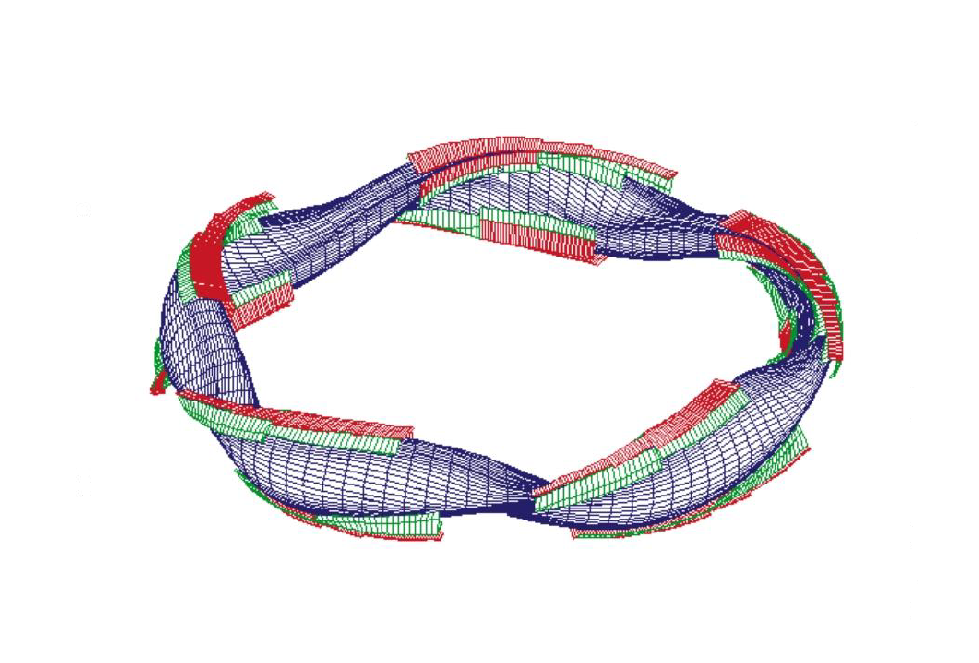
\epsfig{file=documentation/stelldiv.eps,width=160mm}}
\caption[Stellarator island divertor configuration]
{\label{fig:stelldiv}
  \textit{A five-period HELIAS plasma (specifically W7-X) with island divertor
    plates shown in red}
}
\end{figure}

Rather than trying to describe the complex physics with a two-point scrape-off
layer model as is used for tokamaks, the stellarator divertor
model~\cite{stell_divertor} is based on fundamental principles which relate
the power crossing the separatrix with an effective wetted area on the
divertor plates allowing the code to estimate the heat load delivered to the
divertor. A basic island divertor model is used which assumes diffusive
cross-field transport and high radiation at the X-point,

The radiated power fraction in the scrape-off layer is given by the input
parameter \texttt{f\_rad}. This is in contrast to the method used for
tokamaks, in which the radiated power fraction is a calculated quantity.

A number of other input parameters may be used to modify the divertor model;
see the variable descriptor file for more details.

\subsection{Machine configuration}

There are a large number of possible stellarator configurations. As stated
earlier, the one chosen for the \process\ model is based on the
\textbf{HELI}cal \textbf{A}dvanced \textbf{S}tellarator (HELIAS) concept, in
which all the coils resemble distorted, non-planar TF coils --- no helical
coils or tokamak-like PF coils are present.  The coil geometry is scaled from
the HELIAS 5-B power plant design, which is based on a five field-period
HELIAS configuration.

\subsubsection{Machine build}
\label{sec:stbuild}

Since a stellarator is inherently non-axisymmetric, the build of the \process\
stellarator is defined in terms of the mean thicknesses of components.

The surface areas for the first wall, blanket and shield components are scaled
linearly with their effective minor radius from the plasma surface area
calculation (the area of a simple torus of circular cross-section is $4 \pi^2
R a$, hence the linear scaling with $a$). The input parameter \texttt{fhole}
may be used to specify the hole fraction, to adjust the surface area to
take account of ports and divertors, for instance. The volumes of the first
wall etc.\ are simply given by the product of their surface area and their
mean thickness.

In contrast to tokamaks, which in \process\ are assumed to have a cylindrical
external cryostat completely surrounding the fusion power core, the
stellarator model assumes that the external cryostat (labelled as the outer
vessel in Figure~\ref{fig:helias5b}) is toroidal with a circular
cross-section. Its cross-section is assumed to be centred at the mean plasma
major radius.

All items external to the fusion power core (buildings, turbines, power
conversion systems, etc.) remain unchanged.

\subsubsection{Stellarator coils}

The stellarator coil model~\cite{stell_coil, stell_coil2} combines scaling
aspects based on the HELIAS 5-B design in combination with analytic inductance
and field calculations.

The fully three-dimensional shape of the coils is assumed to be fixed, but the
sizes of the coils are scaled from the HELIAS 5-B values to the geometrical
values for the machine being modelled using fundamental physics and
engineering principles.

The stellarator coils are assumed to be superconducting --- no resistive coil
calculations are performed.  The critical field at the superconductor is
calculated using circular approximations for the coils in the inductance and
field calculations, and the limit is enforced automatically. Available
superconductors are Nb$_3$Sn (\texttt{isumattf = 1}) and NbTi
(\texttt{isumattf = 3}).

The winding pack cross-section is rectangular for the stellarator coils,
rather than the complicated two-step cross-section assumed for tokamaks. The
coil thicknesses and most of the dimensions of the materials within the coil
cross-section are outputs from the model, instead of being inputs as is the
case for tokamaks; see the variable descriptor file for details. In addition,
certain iteration variables (\texttt{tfcth}, no.\ 13; \texttt{thkcas}, no.\
57; \texttt{cpttf}, no.\ 60 and \texttt{tftort}, no.\ 77) should not be turned
on in the input file as they are calculated self-consistently; the code will
stop with an error message if this is attempted.



\section{Safety and Environment Models}

At present, the neutronics, activation and inventory calculations comprise the
safety and environment models in the code.

The models comprising the safety and environmental calculations~\cite{FISPACT}
within the code are all called from routine \texttt{FISPAC}. They are only
performed once, at the end of each run, as they take a relatively long time to
evaluate, and the results are only used for diagnostic purposes --- no
constraints are imposed at present to minimise doses, for instance.
% AND LOCA in safety.f90...

N.B.\ These models are currently not available in the present version of the
code.

\subsection{Neutronics}

The neutronics module predicts the neutron flux spectra in the inboard and
outboard first wall and blanket components. The spectra are based on a
simplified tokamak device that has a fixed ratio ($=1.5825$) between the
outboard blanket thickness and the inboard blanket thickness, and are scaled
according to the actual thickness of the outboard blanket. This relatively
limited, single-parameter approach is expected to be replaced by a more
general method, which should allow a more accurate portrayal of the device
being modelled by \process.

\subsection{Activation and inventory information}

The code evaluates the consequences of exposing the power plant's materials to
the calculated neutron fluxes, subject to the limitations imposed by the
neutronics module. A library of neutron cross-sections and decay data is used
to calculate the total activity, gamma-ray dose rate and decay heat output due
to the materials' exposure to neutrons, both at the end of the plant's life
and at a time 100 years later. These values are relevant to decommissioning
and disposal studies, and additional parameters that can be obtained from the
nuclide inventory will also be included as the need arises.

\section{Cost Models}

Two cost models are available, determined by the switch \texttt{cost\_model}.

\subsection{1990 cost model (\texttt{cost\_model = 0})}

This combines methods~\cite{cost1} used in the TETRA code~\cite{tetra} and the Generomak~\cite{generomak} scheme.  The
costs are split into accounting categories~\cite{cost2}. The best references for the algorithms used are~\cite{storac}, and source file \texttt{costs.f90} in the code itself. The majority of the costed items have a unit cost associated with them. These values scale with (for example) power output, volume, component mass etc., and many are available to be changed via the input file. All costs and their algorithms correspond to 1990 dollars.

The unit costs of the components of the fusion power core are relevant to ``first-of-a-kind'' items. That is to say, the items are assumed to be relatively expensive to build as they are effectively prototypes and specialised tools and machines have perhaps been made specially to create them. However, if a ``production line'' has been set up, and R \& D progress has allowed more experience to be gained in constructing the power core components, the costs will be reduced as a result. Variable \texttt{fkind} may be used to multiply the raw unit costs of the fusion power core items (by a
factor less than one) to simulate this cost reduction for an $N^{th}$-of-a-kind device. In other systems studies of fusion power plants~\cite{galambos}, values for this multiplier have ranged from 0.5 to 0.8.

Many of the unit costs have four possible choices, relating to the level of safety assurance~\cite{lsa} flag \texttt{lsa}. A value \texttt{lsa = 1} corresponds to a plant with a full safety credit (i.e.\ is truly passively safe). Levels \texttt{2} and \texttt{3} lie between the two extremes, and level \texttt{4} corresponds to a present day fission reactor, with no safety credit.

The first wall, blanket, divertor, centrepost (if present) and current drive system have relatively short lifetimes because of their hostile environment, after which they must be replaced. Because of this frequent renewal they can be regarded as though they are ``fuel'' items, and can be costed accordingly. Switch \texttt{ifueltyp} is used to control whether this option is used in the code. If \texttt{ifueltyp = 1}, the costs of the first wall, blanket, divertor and a fraction \texttt{fcdfuel} of the cost of the current drive system are treated as fuel costs. If \texttt{ifueltyp = 0}, these are treated as capital costs.

If the switch \texttt{ireactor = 0}, no cost of electricity calculation is performed. If \texttt{ireactor = 1}, then the cost of electricity is evaluated, with the value quoted in units of \$/MWh.

The net electric power is calculated in routine \texttt{POWER}. It is possible that the net electric power can become negative due to a high recirculating power. Switch \texttt{ipnet} determines whether the net electric power is scaled to always remain positive (\texttt{ipnet = 0}), or whether it is allowed to become negative (\texttt{ipnet = 1}), in which case no cost of electricity calculation is performed.

\subsection{2015 Kovari model (\texttt{cost\_model = 1})}
This model~\cite{kovari_cost} provides only capital cost, and is not currently suitable for estimating the cost of electricity.  $N^{th}$-of-a-kind factors, level of safety assurance factors, and blanket replacement costs are not included.  The mean electric output is calculated using the capacity factor, which takes accountof the availability and the dwell time for a pulsed reactor.  The capital cost divided by the mean electric output is a useful comparison parameter.

\section{Plant availability}

Switch \texttt{iavail} is used to control how the overall plant availability
factor \texttt{cfactr} is calculated, as follows

If \texttt{iavail = 0}, the input value of \texttt cfactr is used.

If \texttt{iavail = 1}, a model by N.~Taylor and D.~Ward~\cite{TaylorWard_avail1999} is used instead, in which \texttt{cfactr} is calculated taking into account the time taken to replace certain components of the fusion power core, and various unplanned unavailability fractions which may be set by the user, as summarised in Table~\ref{tab:availability}.
\begin{table}[tbph]
\begin{center}
\begin{tabular}{||c|c||} \hline
input parameter & description \\ \hline
\texttt{tbktrepl}  & time needed to replace blanket (years) \\
\texttt{tdivrepl} & time needed to replace divertor (years) \\
\texttt{tcomrepl} & time needed to replace both blanket and divertor (years) \\
\texttt{uubop} & unplanned unavailability of balance of plant \\
\texttt{uucd} & unplanned unavailability of current drive system \\
\texttt{uudiv} & unplanned unavailability of divertor \\
\texttt{uufuel} & unplanned unavailability of fuelling system \\
\texttt{uufw} & unplanned unavailability of first wall \\
\texttt{uumag} & unplanned unavailability of magnets \\
\texttt{uuves} & unplanned unavailability of vessel \\
\hline
\end{tabular}
\end{center}
\caption[Parameters used in the Taylor-Ward availability model]
{\label{tab:availability}
  \textit{Summary of the variables in PROCESS that relate to
    the Taylor-Ward availability model (\texttt{iavail=1}).}
}
\end{table}

If \texttt{iavail = 2}, the new Morris model is implemented \cite{kovari_eng}. It estimates both planned and unplanned unavailability, and the time during which no power is being generated if the reactor is pulsed. 

The planned unavailability is linked to the lifetimes of the blanket and divertor and the time taken to replace them.  The lifetime of the blanket is based on the allowable fast neutron fluence.  In contrast, the lifetime of the divertor is estimated using the particle and photon load. The time to replace the blanket and divertor have been estimated by Crofts et al, who studied the influence of the number of remote handling systems working in parallel.  \process\ uses a simple fit to their results, and adds a month to allow the dose rate to reduce to an acceptable level before remote handling operations start, and a month to allow for pump-down and preparation for operation at the end of the shutdown.   

To estimate the unplanned downtime, each susbsystem is represented by a simple model that tries to capture the degradation of reliability when approaching operational and technological limits.  This increases the risk of unplanned downtime as design margins are reduced.

For the toroidal field coils, the chance of a quench is likely to be the largest driver of the risk of unplanned unavailability, and this may depend on the temperature margin - the difference between the actual temperature and the critical temperature of the superconductor.  The user inputs a minimum temperature margin, below which quench is immediate, and a second, higher value, above which quenches never occur.  In between, there is a finite quench rate.

The unplanned downtime for the blanket is based on the number of cycles it experiences before planned replacment.  (This model is restricted to pulsed reactors.) The cycle life of the blanket is expressed using a reference lifetime.  Before this liefetime, there is a constant but small probability of failure in ecah pulse.  After the reference lifetime the reliability of the blanket starts to decline, reaching zero at the upper lifetime limit.

It is assumed that the vacuum system can be maintained in parallel with blanket replacement, so it does not contribute to the planned downtime.  The unplanned downtime is based on an assumed failure rate for a cryopump, and a specified total number of pumps, with some of them being redundant.  The resulting downtime can be reduced to a negligible level if there are several redundant pumps, but in addition, there is a fixed unavailability to allow for common mode failures affecting several pumps.



\mychapter{Running \process}
\label{chap:run}

The intention of this chapter is to provide a comprehensive prescription for
setting up and performing runs with the code.  Firstly, the input file's
structure and format is described. The user is then taken through the
procedure for setting up the code to model a new machine, and finally an
attempt is made to indicate and solve the problems that the user will face
whilst trying to achieve a feasible solution.

\section{Environment set-up}
\label{sec:run_environment}

 \process\ is available for execution from the CCFE Fusion Unix Network, on which you must have an account.

To set up your environment to be able to run the code, the user interface and the associated
utilities (see utilities documentation), add the following lines to your \texttt{.bashrc} file.  This is a file in the user's home directory, assuming the bash Unix shell is being used.  Although hidden, it can be opened by issuing the relevant command, for example \texttt{gedit .bashrc}.
\begin{quote}
\begin{verbatim}
module use /home/PROCESS/modules
module swap python
module load process/master

If using default gfortran compiler instead of ifort:
(module unload ifort/10.0.023)
(module load gcc/4.8.2)
\end{verbatim}
\end{quote}
(If you want to use the latest draft version of the code instead of the latest verified release version, replace \texttt{module load process/master} with \texttt{module load process/develop} above.)

Please note, that if you are a \process\/ developer and you want to set up the right environment for using your local \process\/ version, follow instructions in the utilities documentation.

\section{User Interface}
\label{sec:gui}
The \process\/ graphical user interface (GUI) is currently under construction. The developer guide describes how to set it up and use it. 


\section{Executing the Code}

Execute \process\ by simply typing \texttt{process} on the Unix command line.

By default, the input and output file names are as described in the following
sections. If, however, \process\ is executed with an argument, this is used as
a prefix to the file names:
\begin{quote}
\begin{verbatim}
process myrun
\end{verbatim}
\end{quote}
will assume that the input file is called \textit{myrun}\indat, etc.

The input file must be in the current directory.  The output files \textit{myrun}\outdat\
and \textit{myrun}\mfile\ will be created in the current directory.

\section{The Input File}
\label{sec:infile}

The input file \indat\ is used to change the values of the physics,
engineering and other code parameters from their default values, and to set up
the numerics (constraint equations, iteration variables etc.) required to
define the problem to be solved.  The user interface writes the input file, so
it is not necessary to edit it directly.  Details of layout and format are in
Appendix~\ref{app:infile}.

If the code encounters a problem reading the input file, it will stop
immediately with an error message. The last line of the output file \outdat\
may give an indication of where in the input file the problem lies.

\section{The Output Files}

The main output from the code is sent to file \outdat\ in the working
directory.  It is essential to check that the code reports that it has found a
\textit{feasible solution}.

A second file, \mfile, is also produced in the working directory.  This file
contains most of the same data as \outdat\ but in a different format, and has
been designed to be ``machine-readable'' by some of the utility programs
described in the utilities documentation, to allow simple post-processing and
graphical output to be produced easily.

Radial profiles produced by PLASMOD (see section~\ref{sec:plasmod}) are stored in
output file \radpdat. 

\section{Optimisation mode}

Switch \texttt{ioptimz} should be set to \texttt{1} for optimisation mode.

If \texttt{ioptimz = 0}, a non-optimisation pass is performed first.  Occasionally this provides a feasible set of initial conditions that aids convergence of the optimiser, but it is recommended to use \texttt{ioptimz = 1}.

Enable all the relevant consistency equations, and it is advisable to enable the corresponding iteration variables shown first as corresponding itvs in the vardes.html file. A number of limit equations (inequality constraints) can also be activated.  For limit equations, the corresponding f-value must be selected as an iteration variable.  In optimisation mode, the number of iteration variables is unlimited.

It may still be difficult, if not impossible, to reconcile the fusion power
and the net electric power with the required values. This may well be due to
the power conversion efficiency values being used --- refer to
Figure~\ref{fig:powerflow3}.

With luck, a few iterations of this process will produce an adequate benchmark
case. A typical input file for use with \process\ in non-optimisation mode is
contained in Appendix~\ref{app:infile1}.

If scans of a given variable are to be made over a large range of
values, it is often a good idea to start the scan in the middle of the desired
range, and to split the scan in two --- one going downwards from the initial
value, and the other upwards.  This ensures that the whole range of the scan
produces well-converged machines (assuming a ``good'' initial point), without
sharp changes in gradient in the parameter values.

It should be remembered that the value of the scan variable is set in the
array \texttt{sweep}, and this overrules any value set for the variable
elsewhere in the input file.

The output from an optimisation run contains an indication as to which iteration variables lie at their limiting values. A typical input file for use with \process\ in optimisation mode is contained in Appendix~\ref{app:infile2}.

\section{Non-optimisation mode}
\label{sec:optim}

Non-optimisation mode is sometimes used to perform benchmark comparisons, whereby the
machine size, output power etc.\ are known and one only wishes to find the
calculated stresses, beta values and fusion powers, for example.

Running \process\ in non-optimisation mode requires few changes to be made to the
input file from the non-optimisation case. The main differences between
optimisation mode and non-optimisation mode are:

\begin{enumerate}

\item Non-optimisation mode does NOT apply lower or upper bounds to the iteration
  variables.  It follows that limit equations are not enforced.

\item In non-optimisation mode the number of active iteration variables must be equal to the number of constraints.

\item A figure of merit is not available in non-optimisation mode.

\item Scans cannot be performed in non-optimisation mode.

\end{enumerate}

As before, the user must decide which constraint equations and iteration
variables to activate.


\section{Troubleshooting}
\label{sec:problems}

Experience has shown that the first few attempts at running \process\ with a
new input file tends to produce unfeasible results --- that is, the code will
not find a consistent set of machine parameters. The highly non-linear nature
of the numerics of \process\ is the reason for this difficulty, and it often
requires a great deal of painstaking adjustment of the input file to overcome.  The utility
\texttt{a\_to\_b} (see utilities documentation) is useful in this situation.

\subsection{Error handling}
\label{sec:errors}

In general, errors detected during a run are handled in a consistent manner,
with the code producing (hopefully) useful diagnostic messages to help the
user understand what has happened.

There are three levels of errors and warning that may occur:
\begin{description}

\item{Level 1:} An \textit{informational}\/ message is produced under certain
  conditions, for example if the code has modified the user's input choice for
  some reason.

\item{Level 2:} A \textit{warning}\/ message is produced if a non-fatal situation has
  occurred that may result in an output case that is inaccurate or
  unreliable in some way.

\item{Level 3:} An \textit{error}\/ message will occur if a severe or fatal
  error has occurred and the program cannot continue.

\end{description}

These messages are printed on the screen during the course of a run, and those
still active at the final (feasible or unfeasible) solution point are also
written to the end of the output file (messages encountered during the
iteration process are not copied to the output file, as the convergence to a
valid solution might resolve some of the warnings produced earlier in the
solution process).

The \texttt{error\_status} variable returns the highest severity level that
has been encountered (or zero if no abnormal conditions have been found); if a
severe error (level 3) is flagged at any point the program is terminated
immediately. The final message number encountered during a run is returned via
output variable \texttt{error\_id}. In addition, with certain messages, a
number of diagnostic values may also be given; these can be used to provide
extra diagnostic information if the source code is available.

\subsection{General problems}

A code of the size and complexity of \process\ contains myriads of equations
and variables. Virtually everything depends indirectly on everything else
because of the nature of the code structure, so perhaps it is not surprising
that it is often difficult to achieve a successful outcome.

Naturally, problems will occur if some of the parameters become unphysical.
For example, if the aspect ratio becomes less than or equal to one, then we
must expect problems to appear. For this reason, the bounds on the
iteration variables should be selected with care.

Occasionally arithmetic (``\texttt{NaN}'') errors are reported. They usually occur when the code is exploring unphysical values of the parameters, and often suggest that no feasible solution exists for the input file used.

The error messages produced by the code attempt to provide diagnostic
information, telling the user where the problem occurs, and also suggest a
possible solution. These messages are out of necessity brief, and so cannot
promise to lead to a more successful outcome.

There is the option to turn on extra debugging output; to do this, set \texttt{verbose = 1} in the input file.

\subsection{Optimisation problems}

On reflection it is perhaps surprising that \process\ ever does manage to
find the global minimum figure of merit value, since if there are
\texttt{nvar} iteration variables active the search is over
\texttt{nvar}-dimensional parameter space, in which there may be many shallow
minima of approximately equal depth. Remember that \texttt{nvar} is usually of
the order of twenty.

The machine found by \process\ may not, therefore, be the absolutely optimal
device. It is quite easy to have two or more solutions, with results only a
few per cent different, but a long way apart in parameter space. The technique
of ``stationary'' scans is sometimes used in this situation: a scan is requested, but the same value of the scan variable is listed repeatedly.

Scans should be started in the middle of a range of values, to try to keep the
scan within the same family of machines. The optimum machine found may
otherwise suddenly jump to a new region of parameter space, causing the output
variables to seem to vary unpredictably with the scanning variable.

It should be noted that in general the machine produced by \process\ will
always sit against one or more operation limits. If, during a scan, the limit
being leant upon changes (i.e.\ if the machine jumps from leaning on the beta
limit to leaning on the density limit) the output parameters may well become
discontinuous in gradient, and trends may suddenly change direction.

\subsection{Unfeasible results}

In the numerics section of the output file, the code indicates whether the run
produced a feasible or unfeasible result.

The former implies a successful outcome, although it is always worth checking
that the sum of the squares of the constraint residuals (\texttt{sqsumsq}) is small ($\sim
10^{-3}$ or less); the code will issue a warning if the solver reports convergence but
the value of \texttt{sqsumsq} exceeds $10^{-2}$. If this occurs, reducing the
value of the HYBRD tolerance \texttt{ftol} or \vmcon\ tolerance
\texttt{epsvmc} as appropriate should indicate whether the result is valid
or not; the output can usually be trusted if (1) the constraint
residues\footnote{The constraint residues are the final values of $c_i$ in the
  constraint equations --- see Section~\ref{sec:constraints}. The value
  \texttt{sqsumsq} is the square root of the sum of the squares of these
  residuals.} fall as the tolerance is reduced to about $10^{-8}$, and (2) the
code indicates that a feasible solution is still found.

An unfeasible result occurs if \process\ cannot find a set of values for the
iteration variables which satisfies all the given constraints. In this case,
the values of the constraint residues shown in the output give some indication
of which constraint equations are not being satisfied --- those with the
highest residues should be examined further. In optimisation mode, the code
also indicates which iteration variables lie at the edge of their allowed
range.

Unfeasible runs can be caused by specifying physically incompatible input parameters,  using insufficient iteration variables, or by starting the problem with unsuitable values of the iteration variables.

The utility \texttt{run\_process} (see utilities documentation) carries out many runs, changing the starting values of the iteration variables randomly.  It stops once a feasible solution is found.

Another approach is to start with an input file that gives a feasible solution, and modify it step by step towards the parameters desired.  This process is automated by the
utility \texttt{a\_to\_b} (see utilities documentation).

It is important to choose the right number of \textit{useful}\/ iteration variables for the
problem to be solved --- it is possible to activate too many iteration variables as well as too few, some of which may be redundant.

Both optimisation and non-optimisation runs can fail with an error message
suggesting that the iteration process is not making good progress. This is
likely to be due to the code finding itself unable to escape a region of the
parameter space where the minimum in the residuals is significantly above
zero. In this situation, there is either no solution possible (the residuals
can therefore never approach zero), or the topology of the local minimum makes
it difficult for the code to escape to the global minimum. Again, a helpful
technique is to either change the list of iteration variables in use, or to
simply modify their initial values to try to help the code avoid such regions.

A technique that occasionally removes problems due to unfeasible results,
particularly if an error code \texttt{ifail = 3} is encountered during an
optimisation run, is to adjust slightly one of the limits imposed on the
iteration variables, even if the limit in question has not been reached. This
subtly alters the gradients computed by the code during the iteration process,
and may tip the balance so that the code decides that the device produced is
feasible after all. For instance, a certain component's temperature might be
400~K, and its maximum allowable temperature is 1000~K\@. Adjusting this limit
to 900~K (which will make no difference to the \textit{actual}\/ temperature)
may be enough to persuade the code that it has found a feasible solution.

Similarly, the order in which the constraint equations and iteration variables
are stored in the \texttt{icc} and \texttt{ixc} arrays can make the difference
between a feasible and unfeasible result. This seemingly illogical behaviour
is, sadly, typical of the way in which the code works.

Another technique in such situations may be to change the finite difference
step length \texttt{epsfcn}, as this might subtly change the path taken in the
approach towards a solution.

It may be the case that the act of satisfying all the required constraints is
impossible. No machine can exist if the allowed operating regime is too
restrictive, or if two constraint equations require conflicting
(non-overlapping) parameter spaces. In this case some relaxation of the
requirements is needed for the code to produce a successful machine design.

\subsection{Hints}

The above sections should indicate that it is the complex interplay between
the constraint equations and the iteration variables that determines whether
the code will be successful at producing a useful result. It can be a somewhat
laborious process to arrive at a working case, and (unfortunately, perhaps)
experience is often of great value in this situation.

It should be remembered that sufficient iteration variables should be used to
solve each constraint equation. For instance, a particular limit equation may
be $A \leq B$, i.e.\ $A = fB$, where the f-value $f$ must lie between zero and
one for the relation to be satisfied.  However, if none of the iteration
variables have any effect on the values of $A$ and $B$, and $A$ happens to be
\textit{greater}\/ than $B$, then \process\ will clearly not be able to solve
the constraint.

The lower and upper bounds of the iteration variables are all available to be
changed in the input file. Constraints can be relaxed in a controlled manner
by moving these bounds, although in some cases care should be taken to ensure
that unphysical values cannot occur.  The code indicates which iteration
variables lie at the edge of their range.

It is suggested that constraint equations should be added one at a time, with
sufficient new iteration variables activated at each step.  If the situation
becomes unfeasible it can be helpful to reset the initial iteration variable
values to those shown in the output from a previous feasible case, and rerun
the code.

\mychapter{Acknowledgements \& Bibliography}
\label{chap:acks}

The authors would like to thank the following people for many useful
and revealing discussions during their work on \process:

\begin{itemize}
\item[---]
John D.\ Galambos, Paul C.\ Shipe and Y-K.\ Martin Peng of Oak Ridge
National Laboratory, USA;
\item[---]
Ian Cook, Robin Forrest, Winston Han, Roger Hancox and Panos Karditsas, all formerly of
Fusion Physics Department, UKAEA Fusion;
\item[---]
John Hicks, formerly of Engineering Department, UKAEA Fusion;
\item[---]
Chris Gardner, formerly of Microwave and Interpretation Department, UKAEA
Fusion;
\item[---]
Tim Hender of CCFE, and all the co-authors of reference~\cite{172};
\item[---]
David Ward, Richard Kemp and Neill Taylor, all of
CCFE, and the members of the \process\ User Group throughout Europe.
\end{itemize}

This work was funded by the RCUK Energy Programme under grant EP/I501045 and
the European Communities under the contract of Association between EURATOM and
CCFE\@. The views and opinions expressed herein do not necessarily reflect those
of the European Commission. Part of this work was carried out within the
framework of the European Fusion Development Agreement.

\begin{thebibliography}{99}
\raggedright

\bibitem{tetra}
R.\ L.\ Reid et al.,
\textit{``ETR/ITER Systems Code''},
Oak Ridge Report ORNL/FEDC-87/7
(1988)

\bibitem{storac}
J.\ D.\ Galambos,
\textit{``STAR Code : Spherical Tokamak Analysis and Reactor Code''},
Unpublished internal Oak Ridge document. A copy exists in the \process\
Project Work File~\cite{PWF}.

\bibitem{hybrd_anl}
J.\ J.\ More, B.\ S.\ Garbow and E.\ Hillstrom,
\textit{``User Guide for MINPAC-1''},
Argonne National Laboratory Report ANL-80-74
(1980)

\bibitem{hybrd}
M.\ J.\ D.\ Powell,
\textit{``A Hybrid Method for Non-linear Algebraic Equations''},
Numerical Methods for Non-linear Algebraic Equations, ed.\ P.\ Rabinowitz,
Prentice-Hall

\bibitem{vmcon}
R.\ L.\ Crane, K.\ E.\ Hillstrom and M.\ Minkoff,
\textit{``Solution of the General Nonlinear Programming Problem with
Subroutine VMCON''},
Argonne National Laboratory Report ANL-80-64
(1980)

\bibitem{Powell1978}
M.\ J.\ D.\ Powell,
\textit{``A Fast Algorithm for Nonlinearly Constrained Optimization Calculations''},
Lecture Notes in Mathematics, vol. 630, pp.144--157, Springer-Verlag, Berlin, 1978

\bibitem{Avriel2003}
M.\ Avriel,
\textit{``Nonlinear Programming: Analysis and Methods''},
Dover Publications, Inc., Mineola, NY, 2003

\bibitem{fwbsshape}
P.\ J.\ Knight,
\textit{``Surface Area and Volume Calculations for Toroidal Shells''},
CCFE internal note T\&M/PKNIGHT/PROCESS/009, May 2013

\bibitem{Zohm}
H.\ Zohm et al,
\textit{``On the Physics Guidelines for a Tokamak DEMO''},
FTP/3-3, Proc. IAEA Fusion Energy Conference, October 2012, San Diego

\bibitem{DEMOPhysicsGuidelines}
T.\ Hartmann and H.\ Zohm,
\textit{``Towards a `Physics Design Guidelines for a DEMO Tokamak'
  Document''},
EFDA Report, March 2012 (Activity\_3\_Physics\_Design\_Guidelines\_2L8QVN\_v1\_0(1).pdf)

\bibitem{Sakamoto}
Y.\ Sakamoto,
\textit{``Recent progress in vertical stability analysis in JA''},
Task meeting EU-JA\#16, Fusion for Energy, Garching, 24--25 June 2014

\bibitem{logbook14_41}
P.\ J.\ Knight, CCFE Logbook, F/MI/PJK/LOGBOOK14, pp.41--43

\bibitem{BoschHale}
H.-S.\ Bosch and G.\ M.\ Hale,
\textit{``Improved Formulas for Fusion Cross-sections and Thermal Reactivities''},
Nuclear Fusion \textbf{32} (1992) 611

\bibitem{helios} 
J.\ Johner,
\textit{``Helios: A Zero-Dimensional Tool for Next Step and Reactor Studies''},
Fusion Science and Technology \textbf{59} (2011) 308--349

\bibitem{Bernert} 
M.\ Bernert,
\textit{``Analysis of the H-mode density limit in the ASDEX Upgrade tokamak using bolometry''},
PhD Thesis LMU München (http://edoc.ub.uni-muenchen.de/16262/) and M. Bernert et al. Plasma Phys. Control. Fus. \textbf{57} (2015) 014038, doi:10.1088/0741-3335/57/1/014038

\bibitem{IPDG}
N.\ A.\ Uckan and ITER Physics Group,
\textit{``ITER Physics Design Guidelines: 1989''},
ITER Documentation Series, No.\ 10, IAEA/ITER/DS/10
(1990)

\bibitem{172}
T.\ C.\ Hender, M.\ K.\ Bevir, M.\ Cox, R.\ J.\ Hastie, P.\ J.\
Knight, C.\ N.\ Lashmore-Davies, B.\ Lloyd, G.\ P.\ Maddison, A.\ W.\
Morris, M.\ R.\ O'Brien, M.\ F.\ Turner and H.\ R.\ Wilson,
\textit{``Physics Assessment for the European Reactor Study''},
AEA Fusion Report AEA FUS 172
(1992)

\bibitem{Ward_fastalpha2006}
D.\ J.\ Ward,
\textit{``PROCESS Fast Alpha Pressure''},
Work File Note F/PL/PJK/PROCESS/CODE/050

\bibitem{kovari_physics}
M.\ Kovari, R.\ Kemp, H.\ Lux, P.\ Knight, J.\ Morris, D.\ J.\ Ward
\textit{``PROCESS: a systems code for fusion power plants - Part 1: Physics''},
Fusion Engineering and Design 89, 3054–3069 (2014), 
http://dx.doi.org/10.1016/j.fusengdes.2014.09.018

\bibitem{kovari_eng}
M.~Kovari, F.~Fox, C.~Harrington, R.~Kembleton, P.~Knight, H.~Lux, J.~Morris
\textit{``PROCESS: a systems code for fusion power plants - Part 2: Engineering''}, Fus. Eng. \& Des. 104, 9-20 (2016)


\bibitem{kovari_cost}
M.\ Kovari et al.,
\textit{``The cost of a fusion power plant: extrapolation from ITER''},
in preparation (2015)

\bibitem{hanni_radiation}
H.~Lux, R.~Kemp, D.J.~Ward, M.~Sertoli
\textit{``Impurity radiation in DEMO systems modelling''},
Fus. Eng. \& Des. 101, 42-51 (2015)

\bibitem{Lux2016}
H.~Lux, R.~Kemp, E.~Fable, R.~Wenninger,
\textit{``Radiation and confinement in 0D fusion systems codes''},
 PPCF, 58, 7, 075001 (2016)


\bibitem{albajar}
Albajar,
Nuclear Fusion \textbf{41} (2001) 665

\bibitem{fidone}
Fidone, Giruzzi and Granata,
Nuclear Fusion \textbf{41} (2001) 1755

\bibitem{Uckan88}
N.\ A.\ Uckan,
Fusion Technology \textbf{14} (1988) 299

\bibitem{Nevins}
W.\ M.\ Nevins et al.,
\textit{``Summary Report: ITER Specialists' Meeting on Heating and
Current Drive''},
ITER-TN-PH-8-4,
13--17 June 1988, Garching, FRG

\bibitem{WilsonBS}
H.\ R.\ Wilson,
Nuclear Fusion \textbf{32} (1992) 257

\bibitem{SauterBS}
O.\ Sauter, C.\ Angioni and Y.\ R.\ Lin-Liu,
Physics of Plasmas \textbf{6} (1999) 2834

\bibitem{SauterBS_errata}
O.\ Sauter, C.\ Angioni and Y.\ R.\ Lin-Liu,
Physics of Plasmas \textbf{9} (2002) 5140

\bibitem{Uckan}
N.\ A.\ Uckan et al.,
Fusion Technology \textbf{13} (1988) 411

\bibitem{efda_blanket_model}
A.\ Li~Puma, F.\ Franza and L.\ V.\ Boccaccini, \textit{``WP12-SYS01-T02 -
  Model Improvements (Blanket Model)''},
EFDA\_D\_2LKMCT, v1.0, EFDA Power Plant Physics \& Technology, February 2013

\bibitem{Harrington_bop}
C.\ Harrington,
\textit{``Development and Implementation of Improved
  Balance of Plant Models for PROCESS''},
CCFE C5.M15 Milestone Report, August 2014 (copy stored as CCFE internal note
T\&M/PKNIGHT/PROCESS/027)

\bibitem{iter_nb3sn}
L.\ Bottura,
\textit{``$J_c(B,T,\epsilon)$ Parameterizations for the ITER Nb$_3$Sn
  Production"},
ITER Document 2MMF7J (2008),
\texttt{https://user.iter.org/?uid=2MMF7J\&action=get\_document}

\bibitem{Myall}
J.\ Myall,
ORNL internal note, 28th August 1987; scanned copy available in
\texttt{Myall\_1987\_TF\_stress\_calc.pdf}

\bibitem{Morris_tfc}
J.\ Morris,
\textit{``PROCESS Superconducting Toroidal Field Coil Model''},
CCFE internal note, 1st May 2014

\bibitem{PWF}
P.\ J.\ Knight,
\textit{``\process\ Reactor Systems Code''},
AEA Fusion Project Work File, F/RS/CIRE5523/PWF
(1992)

\bibitem{tart}
Y-K.\ M.\ Peng and J.\ B.\ Hicks,
\textit{``Engineering Feasibility of Tight Aspect Ratio Tokamak
(Spherical Torus) Reactors''},
AEA Fusion Report AEA FUS 64 (1990)

\bibitem{ELECTROWATT}
\textit{``Pulsed Fusion Reactor Study''},
AEA Fusion Report AEA FUS 205
(1992)

\bibitem{helias5b}
F.\ Schauer, K.\ Egorov and V.\ Bykov,
\textit{``HELIAS 5-B magnet system structure and maintenance concept''},
Fusion Engineering and Design \texttt{88} (2013) 1619--1622

\bibitem{stell_geometry}
F.\ Warmer,
\textit{``Stellarator Plasma Geometry model for the systems code PROCESS''},
IPP Greifswald, Germany, internal note, 19/06/2013

\bibitem{stell_divertor}
F.\ Warmer,
\textit{``Stellarator Divertor model for the systems code PROCESS''},
IPP Greifswald, Germany, internal note, 21/06/2013

\bibitem{stell_coil}
F.\ Warmer and F.\ Schauer,
\textit{``Stellarator Coil model for the systems code PROCESS''},
IPP Greifswald, Germany, internal note, 07/10/2013

\bibitem{vmec}
VMEC MHD force balance code for toroidal domains,
\texttt{http://vmecwiki.pppl.wikispaces.net/VMEC}

\bibitem{geiger}
J.\ Geiger,
\textit{``Darstellung von ineinandergeschachtelten toroidal geschlossenen
  Fl\"{a}chen mit Fourierkoeffizienten''} \textit{``Representation of
  nested, closed surfaces with Fourier coefficients''}
IPP Greifswald, Germany, internal document, 06/07/2010

\bibitem{Nuhrenberg}
%%MHD-Theoretical Aspects of Stellarators
J.\ N\"{u}hrenberg et al., \textit{Plasma Physics and Controlled Fusion},
\textbf{35} (1993) B115

\bibitem{LHD}
S.\ Sudo, Y.\ Takeiri, H.\ Zushi et al., \textit{Nuclear Fusion}, \textbf{30} (1990)
11

\bibitem{Goldston}
R.\ J.\ Goldston, H.\ Biglari, G.\ W.\ Hammett et al.,
\textit{Bull.\ Am.\ Phys.\ Society}, \textbf{34} (1989) 1964

\bibitem{LacknerGottardi}
K.\ Lackner and N.\ A.\ O.\ Gottardi,
\textit{Nuclear Fusion}, \textbf{30} (1990) 767

\bibitem{Stroth}
U.\ Stroth et al.,
\textit{Nuclear Fusion}, \textbf{36} (1996) 1063

\bibitem{Yamada}
H.\ Yamada et al.,
\textit{Nuclear Fusion}, \textbf{45} (2005) 1684

\bibitem{stell_coil2}
F.\ Warmer,
\textit{``Stellarator Modular Coil model for the systems code PROCESS''},
IPP Greifswald, Germany, internal note, 31/07/2013


\bibitem{FISPACT}
N.\ P.\ Taylor, R.\ A.\ Forrest, P.\ J.\ Knight and L.\ J.\ Baker,
\textit{``Safety and Environmental Modelling in the PROCESS Code''},
Strategic Studies Note 94/14 (1994)

\bibitem{cost1}
R.\ L.\ Reid and Y-K.\ M.\ Peng,
\textit{``Potential Minimum Cost of Electricity of Superconducting Coil
Tokamak Power Reactors''},
Proceedings of 13th IEEE Symposium on Fusion Engineering, Knoxville,
Tennessee, October 1989, p.\ 258

\bibitem{generomak}
J.\ Sheffield et al.,
\textit{``Cost Assessment of a Generic Magnetic Fusion Reactor''},
\textit{Fusion Technology} \textbf{9} (1986) 199

\bibitem{cost2}
S.\ Thompson,
\textit{``Systems Code Cost Accounting''},
memo FEDC-M-88-SE,-004 (1988)

\bibitem{galambos}
J.\ D.\ Galambos, L.\ J.\ Perkins, S.\ W.\ Haney and J.\ Mandrekas,
\textit{Nuclear Fusion}, \textbf{35} (1995) 551

\bibitem{lsa}
J.\ P.\ Holdren et al.,
\textit{``Report of the Senior Committee on Environmental Safety and
Economic Aspects of Magnetic Fusion Energy''},
\textit{Fusion Technology}, \textbf{13} (1988) 7

\bibitem{TaylorWard_avail1999}
P.\ J.\ Knight,
\textit{``PROCESS 3020: Plant Availability Model''},
Work File Note F/PL/PJK/PROCESS/CODE/043

\bibitem{git}
\href{http://git-scm.com/}{Git version control system}
\url{http://git-scm.com/}

\bibitem{Powell1964}
M.\ J.\ D.\ Powell,
\textit{``An efficient method for finding the minimum of a function of several
  variables without calculating derivatives''}, 
\textit{Computer Journal}, \textbf{7} No.\ 2 (1964) 155--162

\bibitem{Han1975}
S.-P.\ Han,
\textit{``A Globally Convergent Method for Nonlinear Programming''},
Department for Computer Science, Cornell University, Report 75-257 (1975)

\bibitem{Bazaraa1993}
M.\ S.\ Bazaraa, H.\ D.\ Sherali and C.\ M.\ Shetty,
\textit{``Nonlinear Programming: Theory and Algorithms''},
John Wiley \& Sons, Inc., New York, 1993

\bibitem{Fletcher1970a}
R.\ Fletcher,
\textit{``A General Quadratic Programming Algorithm''},
Atomic Energy Research Establishment, Report T.P.~401, March 1970

\bibitem{Fletcher1970b}
R.\ Fletcher,
\textit{``The calculation of feasible points for linearly constrained
  optimisation problems''},
Atomic Energy Research Establishment, Report R.6354, April 1970

\bibitem{Fletcher1970c}
R.\ Fletcher,
\textit{``A FORTRAN subroutine for general quadratic programming''},
Atomic Energy Research Establishment, Report R.6370, June 1970

\bibitem{Powell1977}
M.\ J.\ D.\ Powell,
\textit{``The convergence of variable metric methods for nonlinearly
  constrained optimisation calculations''},
presented at Nonlinear Programming Symposium 3, Madison, Wisconsin, 1977

\bibitem{WPPMI2014Report}
\textit{``Report on the Systems Code Activities by CCFE in 2014''},
R.\ Kemp, H.\ Lux, J.\ Morris, M.\ Kovari, P.\ Knight et al.,
\href{https://idm.euro-fusion.org/?uid=2M94N2\&version=v1.0\&action=get\_document}
{EuroFusion Report EFDA\_D\_2M94N2 v1.0 - PMI-7.1-2, December 2014}
\url{https://idm.euro-fusion.org/?uid=2M94N2\&version=v1.0\&action=get\_document}

\bibitem{PLASMOD}
E.\ Fable, C.\ Angioni, M.\ Siccinio, H.\ Zohm,
\textit{``Plasma physics for fusion reactor system codes: Framework and model code''},
Fusion Engineering and Design 130, 131-136 (2018)

\bibitem{ASTRA}
G.V.\ Pereverzev, P.N.\ Yushmanov,
\textit{``ASTRA. Automated System for Transport Analysis in a Tokamak''},
Garching: Max-Planck-Institut für Plasmaphysik (2002), presented at IPP 5/98 

\end{thebibliography}

\myappendix{The Input File}
\label{app:infile}

The input file \indat\ is used to change the values of the physics,
engineering and other code parameters from their default values, and to set up
the numerics (constraint equations, iteration variables etc.) required to
define the problem to be solved.  The user interface writes the input file, so it is not necessary to edit it directly.

\subsection{Tokamak or stellarator?}
\label{sec:device}

The default model is the tokamak.  To select a stellarator an additional input file is required, \texttt{device.dat}, which should contain a single character in the first
line, which is interpreted as follows:
\begin{tabbing}
\hspace{15mm}\= \texttt{0} : use tokamak model \\
\> \texttt{1} : use stellarator model \\
\end{tabbing}

\subsection{File format}

Variables can be specified in any order in the input file.  Comment lines start with a \texttt{*} character.  Data lines are of the form
\begin{verbatim}
variable = value
\end{verbatim}
where \texttt{variable} is the name of one of the input parameters or
iteration variables listed in the variable descriptor file, and \texttt{value}
is the (usually numerical) initial value required for that variable. (Arrays,
as opposed to scalar quantities, are treated differently --- see below.) All input data are screened for non-sensible values.

The following rules must be obeyed when writing an input file:

\begin{enumerate}

\item Each variable must be on a separate line.

\item Variable names can be upper case, lower case, or a mixture of both.

\item Spaces may not appear within a variable name or data value.

\item Other spaces within a line, and trailing spaces, are ignored.

\item Commas are not necessary between variables (but see below).

\item Data can extend over more than one line.

\item One-dimensional arrays can be explicitly subscripted, or unscripted, in
  which case the following element order is assumed: \texttt{A(1), A(2),
    A(3),...}

\item At present, multiple dimension arrays can only be handled without
  reference to explicit subscripts, in which case the following element order
  is assumed: \texttt{B(1,1), B(2,1), B(3,1),...} The use of the input file to
  specify multiple dimension array elements is prone to error.

\item Unscripted array elements must be separated by commas.

\item Blank lines are allowed anywhere in the input file.

\item Lines starting with a \texttt{*} are assumed to be comments.

\item Comment lines starting with five or more asterisks (i.e.\
  \texttt{*****}) are reproduced verbatim in the output file. This feature is not recommended, as these comments are likely to become out of date.  The user interface does not support this feature.

\item In-line comments are \textit{usually}\/ ignored, but there can be
  problems if one contains a comma (\texttt{,}). If this is the case, there
  must also be a comma after the variable's value and before the comment.

\end{enumerate}

It is useful to divide the input file into sections, using suitable comment
lines, to help the user keep related variables together.

The following is a valid fragment of an input file (the vertical lines are
simply to help show the column alignment):
\begin{center}
\begin{tabular}{||l}
$\!\!$\texttt{* This line is a comment that will not appear in the output} \\
$\!\!$\texttt{***** This line is a comment that will appear in the output} \\
$\!\!$\texttt{boundl(1) = 2.5,} \\
$\!\!$\texttt{BOUNDU(10) = 3.,} \\
$\!\!$\texttt{BOUNDU(45) = 1,} \\
$\!\!$\texttt{* Another comment... Note that real values can be entered as if} \\
$\!\!$\texttt{* they were integers, and vice versa (but it's not recommended...)} \\
$\!\!$\texttt{epsfcn = 10.e-4,} \\
$\!\!$\texttt{Ftol = 1.D-4,} \\
$\!\!$\texttt{* The next line sets the first five elements of array icc:} \\
$\!\!$\texttt{ICC =   2, 10, 11, 24, 31} \\
$\!\!$\texttt{* The next line sets the first ten elements of array ixc:} \\
$\!\!$\texttt{ixc =   10, 12, 3, 36, 48,} \\
$\!\!$\hspace{15mm}\texttt{1, 2, 6, 13, 16,} \\
$\!\!$\texttt{IOPTIMZ = 1,} \\
$\!\!$\texttt{maxcal = 200} \\
$\!\!$\texttt{ nsweep = 7} \\
$\!\!$\texttt{NEQNS = 5,    This is an in-line comment} \\
$\!\!$\texttt{NVAR = 10,    Another, but successfully containing a comma!} \\
\end{tabular}
\end{center}

The following are \textit{invalid}\/ entries in the input file
(Q: Why?!):
\begin{center}
\begin{tabular}{||l}
$\!\!$\texttt{boundl(1,1) = 2.5,} \\
$\!\!$\texttt{BOUNDU(N) = 3.,} \\
$\!\!$\texttt{A line of `random' characters like this will clearly wreak havoc} \\
$\!\!$\texttt{eps fcn = 10.e-4, ftol = 1.D-4} \\
$\!\!$\texttt{epsvmc = 1.0 e-4} \\
$\!\!$\texttt{ICC =   2  10  11  24  31} \\
$\!\!$\texttt{IOPTIMZ = 1.0,  This will in fact be okay - but is not recommended} \\
$\!\!$\texttt{NEQNS = 5    An in-line comment on a line with only one comma (,) character} \\
\end{tabular}
\end{center}

If the code encounters a problem reading the input file, it will stop immediately
with a (hopefully) useful error message. It may be worth looking at the
contents of the output file as well, to help narrow down on which line of the
input file the problem might lie.
\normalsize

\myappendix{Optimisation Input File}
\label{app:infile2}

The following is a typical input file used to run \process\ in optimisation
mode. 

\footnotesize
\begin{verbatim}
*****
runtitle = 'Example input file'
*--------------------------------------------------*

*---------------Constraint Equations---------------*
neqns = 18       
icc(1) = 1        * beta (consistency equation)
icc(2) = 2        * global power balance (consistency equation)
icc(3) = 5        * density upper limit
icc(4) = 8        * neutron wall load upper limit
icc(5) = 10       * toroidal field 1/r (consistency equation)
icc(6) = 11       * radial build (consistency equation)
icc(7) = 13       * burn time lower limit (pulse)
icc(8) = 15       * l-h power threshold limit
icc(9) = 16       * net electric power lower limit
icc(10) = 24      * beta upper limit
icc(11) = 26      * central solenoid eof current density upper limit
icc(12) = 27      * central solenoid bop current density upper limit
icc(13) = 30      * injection power upper limit
icc(14) = 31      * tf coil case stress upper limit (sctf)
icc(15) = 32      * tf coil conduit stress upper limit (sctf)
icc(16) = 33      * i_op / i_critical (tf coil) (sctf)
icc(17) = 34      * dump voltage upper limit (sctf)
icc(18) = 35      * j_winding pack/j_protection upper limit (sctf)

*---------------Iteration Variables----------------*
nvar = 31        
ixc(1) = 2        * bt * Toroidal field on axis (t) (iteration variable 2)
boundl(2) = 0.01  
boundu(2) = 100.0  

ixc(2) = 3        * rmajor * Plasma major radius (m) (iteration variable 3)
boundl(3) = 0.1  
boundu(3) = 13.0  

ixc(3) = 4        * te * Volume averaged electron temperature (kev)
boundl(4) = 5.0  
boundu(4) = 150.0  

ixc(4) = 5        * beta * Total plasma beta (iteration variable 5)
boundl(5) = 0.001  
boundu(5) = 1.0  

ixc(5) = 6        * dene * Electron density (/m3) (iteration variable 6)
boundl(6) = 1e+19  
boundu(6) = 1e+21  

ixc(6) = 9        * fdene * F-value for density limit
boundl(9) = 0.001  
boundu(9) = 1.2  

ixc(7) = 10       * hfact * H factor on energy confinement times (iteration variable 10)
boundl(10) = 0.1  
boundu(10) = 1.1  

ixc(8) = 12       * oacdcp * Overall current density in tf coil inboard legs (a/m2)
boundl(12) = 100000.0  
boundu(12) = 150000000.0  

ixc(9) = 13       * tfcth * Inboard tf coil thickness; (centrepost for st) (m)
boundl(13) = 0.5  
boundu(13) = 5.0  

ixc(10) = 14      * fwalld * F-value for minimum wall load
boundl(14) = 0.001  
boundu(14) = 1.0  

ixc(11) = 16      * ohcth * Central solenoid thickness (m)
boundl(16) = 0.001  
boundu(16) = 100.0  

ixc(12) = 18      * q * Safety factor 'near' plasma edge (iteration variable 18)
boundl(18) = 3.0  
boundu(18) = 100.0  

ixc(13) = 29      * bore * Central solenoid inboard radius (m)
boundl(29) = 0.1  
boundu(29) = 10.0  

ixc(14) = 36      * fbetatry * F-value for beta limit
boundl(36) = 0.001  
boundu(36) = 1.0  

ixc(15) = 37      * coheof * Central solenoid overall current density at end of flat-top (a/m2)
boundl(37) = 100000.0  
boundu(37) = 100000000.0  

ixc(16) = 38      * fjohc * F-value for central solenoid current at end-of-flattop
boundl(38) = 0.01  
boundu(38) = 0.25  

ixc(17) = 39      * fjohc0 * F-value for central solenoid current at beginning of pulse
boundl(39) = 0.001  
boundu(39) = 0.25  

ixc(18) = 41      * fcohbop * Ratio of central solenoid overall current density at
boundl(41) = 0.001  
boundu(41) = 1.0  

ixc(19) = 42      * gapoh * Gap between central solenoid and tf coil
boundl(42) = 0.05  
boundu(42) = 0.1  

ixc(20) = 44      * fvsbrnni * Fraction of the plasma current produced by
boundl(44) = 0.001  
boundu(44) = 1.0  

ixc(21) = 48      * fstrcase * F-value for tf coil case stress
boundl(48) = 0.001  
boundu(48) = 1.0  

ixc(22) = 49      * fstrcond * F-value for tf coil conduit stress
boundl(49) = 0.001  
boundu(49) = 1.0  

ixc(23) = 50      * fiooic * F-value for tf coil operating current / critical
boundl(50) = 0.001  
boundu(50) = 0.5  

ixc(24) = 51      * fvdump * F-value for dump voltage
boundl(51) = 0.001  
boundu(51) = 1.0  

ixc(25) = 53      * fjprot * F-value for tf coil winding pack current density
boundl(53) = 0.001  
boundu(53) = 1.0  

ixc(26) = 56      * tdmptf * Dump time for tf coil (s)
boundl(56) = 10.0  
boundu(56) = 1000000.0  

ixc(27) = 57      * thkcas * Inboard tf coil case outer (non-plasma side) thickness (m)
boundl(57) = 0.05  
boundu(57) = 1.0  

ixc(28) = 58      * thwcndut * Tf coil conduit case thickness (m)
boundl(58) = 0.004  
boundu(58) = 1.0  

ixc(29) = 59      * fcutfsu * Copper fraction of cable conductor (tf coils)
boundl(59) = 0.001  
boundu(59) = 1.0  

ixc(30) = 61      * gapds * Gap between inboard vacuum vessel and tf coil (m)
boundl(61) = 0.12  
boundu(61) = 10.0  

ixc(31) = 103     * flhthresh * F-value for l-h power threshold
boundl(103) = 1.0  
boundu(103) = 1000000.0  

*-----------------Build Variables------------------*
blnkith = 0.755  * Inboard blanket thickness (m);
blnkoth = 1.275  * Outboard blanket thickness (m);
bore = 2.5907    * Central solenoid inboard radius (m)
ddwex = 0.15     * External cryostat thickness (m)
ddwi = 0.32      * Vacuum vessel thickness (tf coil / shield) (m)
fwith = 0.025    * Inboard first wall thickness; initial estimate (m)
fwoth = 0.025    * Outboard first wall thickness; initial estimate (m)
gapds = 0.12     * Gap between inboard vacuum vessel and tf coil (m)
gapoh = 0.05     * Gap between central solenoid and tf coil
gapomin = 0.2    * Minimum gap between outboard vacuum vessel and tf coil (m)
ohcth = 0.86365  * Central solenoid thickness (m)
scrapli = 0.225  * Gap between plasma and first wall; inboard side (m)
scraplo = 0.225  * Gap between plasma and first wall; outboard side (m)
shldith = 0.3    * Inboard shield thickness (m)
shldoth = 0.8    * Outboard shield thickness (m)
shldtth = 0.3    * Upper/lower shield thickness (m);
tfcth = 0.79433  * Inboard tf coil thickness; (centrepost for st) (m)
vgap2 = 0.12     * Vertical gap between vacuum vessel and tf coil (m)
vgaptf = 1.6     * Vertical gap between x-point and divertor (m)


*---------------Buildings Variables----------------*


*---------------Constraint Variables---------------*
bmxlim = 14.0    * Maximum peak toroidal field (t)
fbetatry = 0.52645  * F-value for beta limit
fdene = 1.2      * F-value for density limit
fhldiv = 2.0     * F-value for divertor heat load
fjohc = 0.25     * F-value for central solenoid current at end-of-flattop
fjohc0 = 0.25    * F-value for central solenoid current at beginning of pulse
flhthresh = 1.0232  * F-value for l-h power threshold
fpeakb = 0.9229  * F-value for maximum toroidal field
fstrcond = 0.84986  * F-value for tf coil conduit stress
fvdump = 0.96778  * F-value for dump voltage
fwalld = 0.13514  * F-value for minimum wall load
pnetelin = 500.0  * Required net electric power (mw)
pseprmax = 17.0  * Maximum ratio of power crossing the separatrix to
tbrnmn = 7200.0  * Minimum burn time (s)
walalw = 8.0     * Allowable wall-load (mw/m2)


*------------------Cost Variables------------------*
abktflnc = 15.0  * Allowable first wall/blanket neutron
adivflnc = 20.0  * Allowable divertor heat fluence (mw-yr/m2)
fcap0 = 1.15     * Average cost of money for construction of plant
fcap0cp = 1.06   * Average cost of money for replaceable components
fcontng = 0.15   * Project contingency factor
fcr0 = 0.065     * Fixed charge rate during construction
ifueltyp = 1     * Switch * treat blanket divertor; first wall and
lsa = 2          * Level of safety assurance switch
output_costs = 0  * Switch for costs output * do not write cost-related outputs to file;
ratecdol = 0.06  * Effective cost of money in constant dollars
tlife = 40.0     * Plant life (years)
ucblvd = 280.0   * Unit cost for blanket vanadium ($/kg)
ucdiv = 500000.0  * Cost of divertor blade ($)
ucme = 300000000.0  * Unit cost of maintenance equipment ($/w**0;3)


*-------------Current Drive Variables--------------*
bscfmax = 0.99   * Maximum fraction of plasma current from bootstrap;
etanbi = 0.4     * Neutral beam wall plug to injector efficiency
frbeam = 1.0     * R_tangential / r_major for neutral beam injection
pinjalw = 50.0   * Maximum allowable value for injected power (mw)


*----------------Divertor Variables----------------*
anginc = 0.175   * Angle of incidence of field line on plate (rad)
divdum = 1       * Switch for divertor zeff model* 0=calc; 1=input
divfix = 0.621   * Divertor structure vertical thickness (m)
hldivlim = 10.0  * Heat load limit (mw/m2)
ksic = 1.4       * Power fraction for outboard double-null scrape-off plasma
prn1 = 0.4       * N-scrape-off / n-average plasma;
zeffdiv = 3.5    * Zeff in the divertor region (if divdum /= 0)


*------------------Fwbs Variables------------------*
fwclfr = 0.1     * First wall coolant fraction


*-----------------Global Variables-----------------*


*-------------Heat Transport Variables-------------*
etath = 0.375    * Thermal to electric conversion efficiency
fauxbop = 0.032  * Fraction of gross electric power to balance-of-plant
ffwlg = 0.01     * Fraction of first wall / divertor power to low grade heat
htpmw = 155.0    * Heat transport system electrical pump power (mw)


*------------------Ife Variables-------------------*


*------------Impurity Radiation Module-------------*
coreradius = 0.6  * Normalised radius defining the 'core' region
fimp = 1.0, 0.1, 0.0, 0.0, 0.0, 0.0, 0.0, 0.0, 0.0, 0.0, 0.0, 0.0, 0.00044, 5e-05  * Impurity number density fractions relative to electron density
impvar = 13      * Fimp element value to be varied if iteration


*---------------------Numerics---------------------*
ioptimz = 1      * Code operation switch * for no optimisation; hybrd only;
minmax = 1       * Switch for figure-of-merit * major radius
epsvmc = 1e-08   * Error tolerance for vmcon


*----------------Pf Power Variables----------------*


*-----------------Pfcoil Variables-----------------*
coheof = 12994000.0  * Central solenoid overall current density at end of flat-top (a/m2)
cptdin = 42200.0, 42200.0, 42200.0, 42200.0, 43000.0, 43000.0, 43000.0, 43000.0  * Peak current per turn input for pf coil i (a)
fcohbop = 0.93314  * Ratio of central solenoid overall current density at
ipfloc = 2, 2, 3, 3  * Switch for locating scheme of pf coil group i
isumatpf = 3     * Switch for superconductor material in pf coils * nbti;
ncls = 1, 1, 2, 2  * Number of pf coils in group j
ngrp = 4         * Number of groups of pf coils;
ohhghf = 0.9     * Central solenoid height / tf coil internal height
rjconpf = 11000000.0, 11000000.0, 6000000.0, 6000000.0, 8000000.0, 8000000.0, 8000000.0, 8000000.0  * Average winding pack current density of pf coil i (a/m2)
rpf2 = -1.825    * Offset (m) of radial position of ipfloc=2 pf coils
sigpfalw = 300.0  * Allowable stress in pf coils/central solenoid (mpa)
zref = 3.6, 1.2, 1.0, 2.8, 1.0, 1.0, 1.0, 1.0  * Pf coil vertical positioning adjuster


*----------------Physics Variables-----------------*
alphaj = 2.0     * Current profile index;
alphan = 1.0     * Density profile index
alphat = 1.0     * Temperature profile index
aspect = 3.5     * Aspect ratio (iteration variable 1)
beta = 0.034253  * Total plasma beta (iteration variable 5)
bt = 5.3983      * Toroidal field on axis (t) (iteration variable 2)
dene = 8.2808e+19  * Electron density (/m3) (iteration variable 6)
dnbeta = 3.0     * (troyon-like) coefficient for beta scaling;
fkzohm = 1.0245  * Zohm elongation scaling adjustment factor (ishape=2; 3)
fvsbrnni = 0.43898  * Fraction of the plasma current produced by
gamma = 0.3      * Ejima coefficient for resistive startup v-s formula
hfact = 1.1      * H factor on energy confinement times (iteration variable 10)
ibss = 4         * Switch for bootstrap current scaling * for sauter et al scaling
iculbl = 1       * Switch for beta limit scaling * apply limit to thermal beta;
impc = 0.0       * Carbon impurity multiplier (imprad_model=0 only)
impo = 0.0       * Oxygen impurity multiplier (imprad_model=0 only)
neped = 6.78e+19  * Electron density of pedestal (/m3) (ipedestal=1)
nesep = 2e+19    * Electron density at separatrix (/m3) (ipedestal=1)
rhopedn = 0.94   * R/a of density pedestal (ipedestal=1)
rhopedt = 0.94   * R/a of temperature pedestal (ipedestal=1)
teped = 5.5      * Electron temperature of pedestal (kev) (ipedestal=1)
tesep = 0.1      * Electron temperature at separatrix (kev) (ipedestal=1)
ishape = 2       * Switch for plasma cross-sectional shape calculation * set kappa to the natural elongation value (zohm iter scaling);
kappa = 1.7      * Plasma separatrix elongation (calculated if ishape > 0)
rmajor = 8.9216  * Plasma major radius (m) (iteration variable 3)
te = 12.959      * Volume averaged electron temperature (kev)
triang = 0.5     * Plasma separatrix triangularity (calculated if ishape=1; 3 or 4)
zfear = 1        * High-z impurity switch; 0=iron; 1=argon


*-----------------Pulse Variables------------------*
lpulse = 1       * Switch for reactor model * pulsed operation


*------------------Rfp Variables-------------------*


*-------------------Scan Module--------------------*
isweep = 1       * Number of scan points to calculate
nsweep = 1       * Switch denoting quantity to scan * aspect
sweep = 3.1      * Actual values to use in scan


*--------------Stellarator Variables---------------*


*-----------------Tfcoil Variables-----------------*
casths = 0.05    * Inboard tf coil sidewall case thickness (m)
cpttf = 65000.0  * Tf coil current per turn (a)
csytf = 990000000.0  * Yield strength of case (tf coils and cs coils) (pa)
fcutfsu = 0.61471  * Copper fraction of cable conductor (tf coils)
oacdcp = 12367000.0  * Overall current density in tf coil inboard legs (a/m2)
ripmax = 0.6     * Maximum allowable toroidal field ripple amplitude
tfno = 18.0      * Number of tf coils (default = 50 for stellarators)
tftmp = 4.75     * Peak helium coolant temperature in tf coils and pf coils (k)
thicndut = 0.001  * Conduit insulation thickness (m)
thkcas = 0.43968  * Inboard tf coil case outer (non-plasma side) thickness (m)
thwcndut = 0.004  * Tf coil conduit case thickness (m)
tmargmin = 1.7   * Minimum allowable temperature margin (cs and tf coils) (k)
vftf = 0.333     * Coolant fraction of tf coil leg (itfsup=0)


*-----------------Times Variables------------------*
tburn = 10000.0  * Burn time (s) (calculated if lpulse=1)


*-----------------Vacuum Variables-----------------*

\end{verbatim}
\normalsize

\myappendix{Non-optimisation Input File}
\label{app:infile1}

The following is a typical input file used to run \process\ in
non-optimisation mode. Comments in [\ldots] have been added to the right of
each line.

\footnotesize
\begin{verbatim}
* Numerics information                [Comment]

NEQNS = 14,                           [Number of active constraint equations]
NVAR = 14,                            [Number of active iteration variables]
ICC =   1,  2, 10, 11, 7, 16, 24, 5, 31, 32, 33, 34, 35, 36,  [Constraint eqns]
ixc =   5, 10, 12, 3,  7,  6, 36, 9, 48, 49, 50, 51, 53, 54,  [Iteration variables]
IOPTIMZ = -1,                         [Turn off optimisation]
ISWEEP=0                              [No scans (non-optimisation mode)]

* F-values and limits

FBETATRY = 1.0                        [N.B. active iteration variable 36]

* Physics parameters

ASPECT = 3.5,                         [Machine aspect ratio]
BETA = 0.042,                         [N.B. active iteration variable 5]
BT = 6.,                              [Toroidal field on axis]
DENE = 1.5e20,                        [N.B. active iteration variable 6]
FVSBRNNI = 1.0,                       [Non-inductive volt seconds fraction]
DNBETA = 3.5,                         [Beta g coefficient]
HFACT = 2.,                           [N.B. active iteration variable 10]
ICURR = 4,                            [Use ITER current scaling]
ISC = 6,                              [Use ITER 89-P confinement time scaling law]
IINVQD = 1,                           [Use inverse quadrature]
IITER = 1,                            [Use ITER fusion power calculations]
ISHAPE = 0,                           [Use input values for KAPPA and TRIANG]
KAPPA = 2.218,                        [Plasma elongation]
Q = 3.0,                              [Edge safety factor]
RMAJOR = 7.0,                         [N.B. active iteration variable 3]
RNBEAM = 0.0002,                      [N.B. active iteration variable 7]
TBURN = 227.9                         [Burn time]
TE = 15.,                             [Electron temperature]
TRIANG = 0.6                          [Plasma triangularity]

* Current drive parameters

IRFCD = 1,                            [Use current drive]
IEFRF = 5                             [Use ITER neutral beam current drive]
FEFFCD = 3.,                          [Artificially enhance efficiency]

* Divertor parameters

ANGINC=0.262,                         [Angle of incidence of field lines on plate]
PRN1=0.285                            [Density ratio]

* Machine build

BORE = 0.12,                          [Machine bore]
OHCTH = 0.1,                          [central solenoid thickness]
GAPOH = 0.08,                         [Inboard gap]
TFCTH = 0.9,                          [Inboard TF coil leg thickness]
DDWI = 0.07,                          [Vacuum vessel thickness]
SHLDITH = 0.69,                       [Inboard shield thickness]
BLNKITH = 0.115,                      [Inboard blanket thickness]
FWITH = 0.035,                        [Inboard first wall thickness]
SCRAPLI = 0.14,                       [Inboard scrape-off layer thickness]
SCRAPLO = 0.15,                       [Outboard scrape-off layer thickness]
FWOTH = 0.035,                        [Outboard first wall thickness]
BLNKOTH = 0.235,                      [Outboard blanket thickness]
SHLDOTH = 1.05,                       [Outboard shield thickness]
GAPOMIN = 0.21,                       [Outboard gap]
VGAPTF = 0,                           [Vertical gap]

* First wall, blanket, shield parameters

LBLNKT=0                              [Use old blanket model]
DENSTL=7800.                          [Steel density]

* TF coil parameters

OACDCP = 1.4e7,                       [N.B. active iteration variable 12]
ITFSUP = 1,                           [Use superconducting TF coils]
RIPMAX = 5.,                          [Maximum TF ripple]

* PF coil parameters

NGRP = 3,                             [Three groups of PF coils]
IPFLOC = 1,2,3,                       [Locations for each group]
NCLS = 2,2,2,1,                       [Number of coils in each group]
COHEOF = 1.85e7,                      [central solenoid current at End Of Flat-top]
FCOHBOP = 0.9,                        [central solenoid current at Begin. Of Pulse / COHEOF]
ROUTR = 1.5,                          [Radial position for group 3]
ZREF(3) = 2.5,                        [Z position for group 3]
OHHGHF = .71                          [Height ratio central solenoid / TF coil]

* Vacuum system parameters

NTYPE = 1                             [Use cryopump]

* Heat transport parameters

ETATH=0.35                            [Thermal to electric conversion efficiency]
FMGDMW = 0.                           [Power to MGF units]
BASEEL=5.e6                           [Base plant electric load]
ISCENR=2                              [Energy store option]

* Buildings

FNDT = 2.                             [Foundation thickness]
EFLOOR=1.d5                           [Effective total floor space]

* Costs

IREACTOR = 1,                         [Calculate cost of electricity]
IFUELTYP = 0                          [Treat blanket, first wall etc as capital cost]
UCHRS = 87.9,                         [Unit cost of heat rejection system]
UCCPCL1 = 250,                        [Unit cost of high strength tapered copper]
UCCPCLB = 150                         [Unit cost of TF outer leg plate coils]
\end{verbatim}
\normalsize




\end{document}
